%Electro-optic study of AlGaAs coated mirrors

Once mirror coating materials are selected for DRFPMI core optics, another fundamental detector noise limit (like that discussed in \ref{sec:shot_noise} is imposed on the gravitational wave detector in the form of coating thermal noise. For aLIGO $\siotao$ coatings this is represented in \hyperref[sec:ligo_noise]. As aLIGO approaches designed sensitivity, alternative mirror coating solutions are proposed with the primary purpose of pushing down the thermal noise limit for further enhancing detector sensitivity \cite{?}. With the potential to reduce coating Brownian noise by a factor of 10, $\gaas$/$\algaas$ shows promise for next generation detectors; with a potential strain reduction by a factor of 5 \cite{Cole:2013} when compared to the current aLIGO coating thermal noise limit. Though applying crystalline mirror HR coatings to the core optics does introduce new side effects; one being linear electro-optic of $\gaas$/$\algaas$ (dn/dE), also known as the Pockels effect \cite{abernathyposter}. A differential phase noise estimate of ? [m/V], alongside measured ambient field noise of ? [V/m] presents adequate motivation for a thorough study dedicated to the electro-optical properties of $\gaas$/$\algaas$ coatings. This section details such a study: starting with a survey of distinguishing optical and material properties of crystalline materials like $\gaas$ and $\algaas$ by reviewing: light propogation through anistropic materials, and induced optical anisotropy of zincblende materials. Preliminary estimates of the differential phase of light reflected from a $\gaas$/$\algaas$ coating stack caused by electric field noise are computed while considering potential impacts to the current generation gravitational wave detectors. Also discussed is a specific study designed to acquire dn/dE estimates from a calibrated differential length PDH locked signal from a short experimental optical cavity with a primarily normal electric field driven across a HR $\gaas$/$\algaas$ coating ``witness" sample.

\subsection{Anisotropic media}
Unlike isotropic media, we do not assume that the index of refraction of anisotropic media is the same for all chosen wave vectors. This is a direct consequence of the birefringence of anisotropic media; characterized by the dielectric, permittivity, and polarization tensors.

\subsubsection{The Dielectric tensor}
Further elaborating on the nature of a generalized dielectric tensor ($\varepsilon$) for any wavevector is required to proceed:
\begin{equation}\label{eq:3.11}
D_i = \varepsilon_{ij}E_j
\end{equation}
Where D is the displacement vector and E is the electric field vector and $\varepsilon$ is the dielectric tensor. The displacement vector for isotropic media is retrieved when $i = j$ and $\varepsilon_i = \varepsilon$. To further understand the nature of the dielectric tensor we assert Poynting's theorem providing an energy conservation requirement:
\begin{equation}\label{eq:3.12}
\nabla \cdot \vec{S} = \frac{dU}{dt}
\end{equation}
Where $\vec{S} = \vec{E} \times \vec{H}$ is the poynting vector and $U = \frac{1}{8 \pi} \big( \vec{E} \cdot \vec{D} + \vec{B} \cdot \vec{H} \big)$ is the electromagnetic field density. The reader is left to perform the exercise and show that in order for \ref{eq:3.12} to hold true given \ref{eq:3.11}


\begin{equation}
\varepsilon_{ij} = \varepsilon_{ji}
\end{equation}
Demonstrating that the dielectric tensor is symmetric - exhibiting only six unique terms. Diagonalizing the tensor, the presence of two unique eigenvectors and eigenvalues indicates the existance of two eigenpolarizations with paired eigenindices.

%The most general form of the energy density can be geometrically represented as ellipsoid but a coordinate transformation we can diagonalize and realize the principal axes of the dielectric allowing a simpler form of the displacement, and in turn the energy density.

\subsubsection{Monochromatic plane wave propogation}
Revisiting Maxwell's equations for a simple monochromatic plane wave solution provides further direction on how crystalline media may effect incident light. Further elaborating, the following assumptions are made:
\begin{equation}
\vec{E} = E_o e^{(i \omega (\frac{n}{c} \vec{r}\cdot \vec{s}-t))}
\end{equation}
Where $n$ is the index of refraction, $c$ is the speed of light, $\vec{r}$ is the position vector and $\vec{s}$ is the unit wave normal.
\begin{equation}
\nabla \times \vec{H}= \frac{\partial \vec{D}}{\partial t}
\end{equation}
Where $\vec{H}$ is the magnetic field assuming permeability $\mu$, and the generalized displacement vector $\vec{D}$ and electric field vector $\vec{E}$.
\begin{equation}
\nabla \times \vec{E} = -\mu \vec{H}
\end{equation}
Reducing to only the displacement and electric fields:
\begin{equation}\label{eq:3.17}
\vec{D} = \frac{n^2}{\mu}[\vec{E}-\vec{s}(\vec{s}\cdot \vec{E})]
\end{equation}
Maxwell's equations show that the electric field is not necessarily parallel to the displacement field and in most materials with non-zero polarizability tensors and dielectric tensors, it is not. But as specified above, the displacement vector, Electric field and unit wave normal are co-planar while remaining orthogonal to $\vec{H}$. Assuming we are operating within a coordinate system aligned with the principal dielectric axes, we substitute \ref{eq:3.11} into \ref{eq:3.17}:
\begin{equation}\label{eq:3.18}
E_i = \frac{n^2 s_i (\vec{E}\cdot\vec{s})}{n^2 - \mu \varepsilon_i}
\end{equation}

From here it can be shown that for a general plane wave there exist two unique refractive index solutions within the constructed dielectric. Though using this result to show this requires revisiting geometrical conditions that are best visualized using a method introduced in the next section \cite{nye}. \textcolor{red}{See appendix}

\subsubsection{Indicatrix}\label{sec:indicatrix}
The two index solutions for a uniaxial crystal given a general plane wave with unit wave vector $\vec{k}$ can be found via a conveniant geometrical construction known as the ``index ellipsoid". 

\begin{figure}[ht!]
\begin{center}
\includegraphics[width=.85\textwidth]{figs/ALGAAS/indicatrix_alph.pdf}
\end{center}
\caption{A surface of uniform energy density ($U_E$) forming an ellipsoid in D-space for a generalized uniaxial crystal with general wavefront propogation indicated by a plane normal $\hat{k'}$ where the major and minor axes of the ellipse cross section indicate slow and fast axes $n_\beta$ and $n_\alpha$ respectively.}
\label{fig:general_indicatrix}
\end{figure}

The construction begins when considering a constant electric energy density ($U_e$) surface in the $\vec{D}$ space; which forms an ellipsoid: 

\begin{equation}\label{eq:lagr1}
\frac{D_x}{\varepsilon_x} + \frac{D_y}{\varepsilon_y} + \frac{D_z}{\varepsilon_z} = 2 U_e \varepsilon_o
\end{equation}
With redefined coordinates $(\vec{D}/\sqrt{2 U_e \varepsilon_o}) \rightarrow \vec{r}$ and setting $\varepsilon_i = n^2_i$:
\begin{equation}
\frac{x^2}{n_x^2} + \frac{y^2}{n_y^2} + \frac{z^2}{n_z^2} = 1
\end{equation}

This equation for the ellipsoid is known as the indicatrix. Given the co-planar solution demonstrated in the last section, we can impose the normal of the plane $\vec{r} \cdot \vec{s} = 0$:

\begin{equation}\label{eq:lagr2}
\vec{r} \cdot \vec{s} = x s_x + y s_y + z s_z = 0
\end{equation}
Equations \ref{eq:lagr1} and \ref{eq:lagr2} both contribute constraints to the method of finding extrema using Lagrange multipliers for the function:
\begin{equation}
r^2 = x^2 + y^2 + z^2
\end{equation}
The Lagrangian ($\mathcal{L}$) with the introduced multiplers ($\lambda_1$, $\lambda_2$) then becomes:
\begin{equation}
\mathcal{L}(\textcolor{red}{\vec{r},\vec{s}},\lambda_1, \lambda_2) =
x^2 + y^2 + z^2 + \lambda_1 (xs_x + ys_y + zs_z) + \lambda_2 \bigg( \frac{x^2}{\varepsilon_x} + \frac{y^2}{\varepsilon_y} + \frac{z^2}{\varepsilon_z} - 1 \bigg)
\end{equation}
With the generated system of equations from the Lagrange multipler method ($\partial F_i/ \partial x_i = 0$, and $\partial F_j/ \partial \lambda_j$) where index $i =x,y,z$ and $j = 1,2$ we obtain a system of 3 equations:
\begin{equation}
i \bigg(1-\frac{r^2}{\varepsilon_{i}} \bigg) + s_{i} \bigg(\frac{x s_x}{\varepsilon_x} + \frac{y s_y}{\varepsilon_y} + \frac{z s_z}{\varepsilon_z} \bigg) = 0
\end{equation}
The result is verified when substituting $r \rightarrow \frac{\vec{D}}{\sqrt{\vec{E} \cdot \vec{D} \varepsilon_o}}$ back which recovers \ref{eq:3.18}.
\\

\subsection{$\gaas$ and $\algaas$ crystal classification}
The space group of $\gaas$ as well as $\algaasgen$ are within the $F\bar{4}3m$ space group \cite{}. Crystals of this space group are commonly known as zincblende crystals; a common crystal configuration named after zinc sulfide (ZnS). Also categorized as a cubic crystal, their crystallographic structure displays optically isotropic characteristics when stress free and no DC and/or slowly varying electric fields are present.
\satoshi{Is this true?} \textcolor{blue}{Yes. Though the birefringence seen from HR $\gaas$ coatings is said to be due to an ``intrinsic stress" in the high and low index layers. (What is breaking the symmetry to cause this? Heteroepitaxy? Annealing? Defects? Is this birefringence the same for all samples?) I think a dedicated high precision birefringence measurement on multiple samples would be cool.}
\begin{figure}[!ht]
\begin{center}
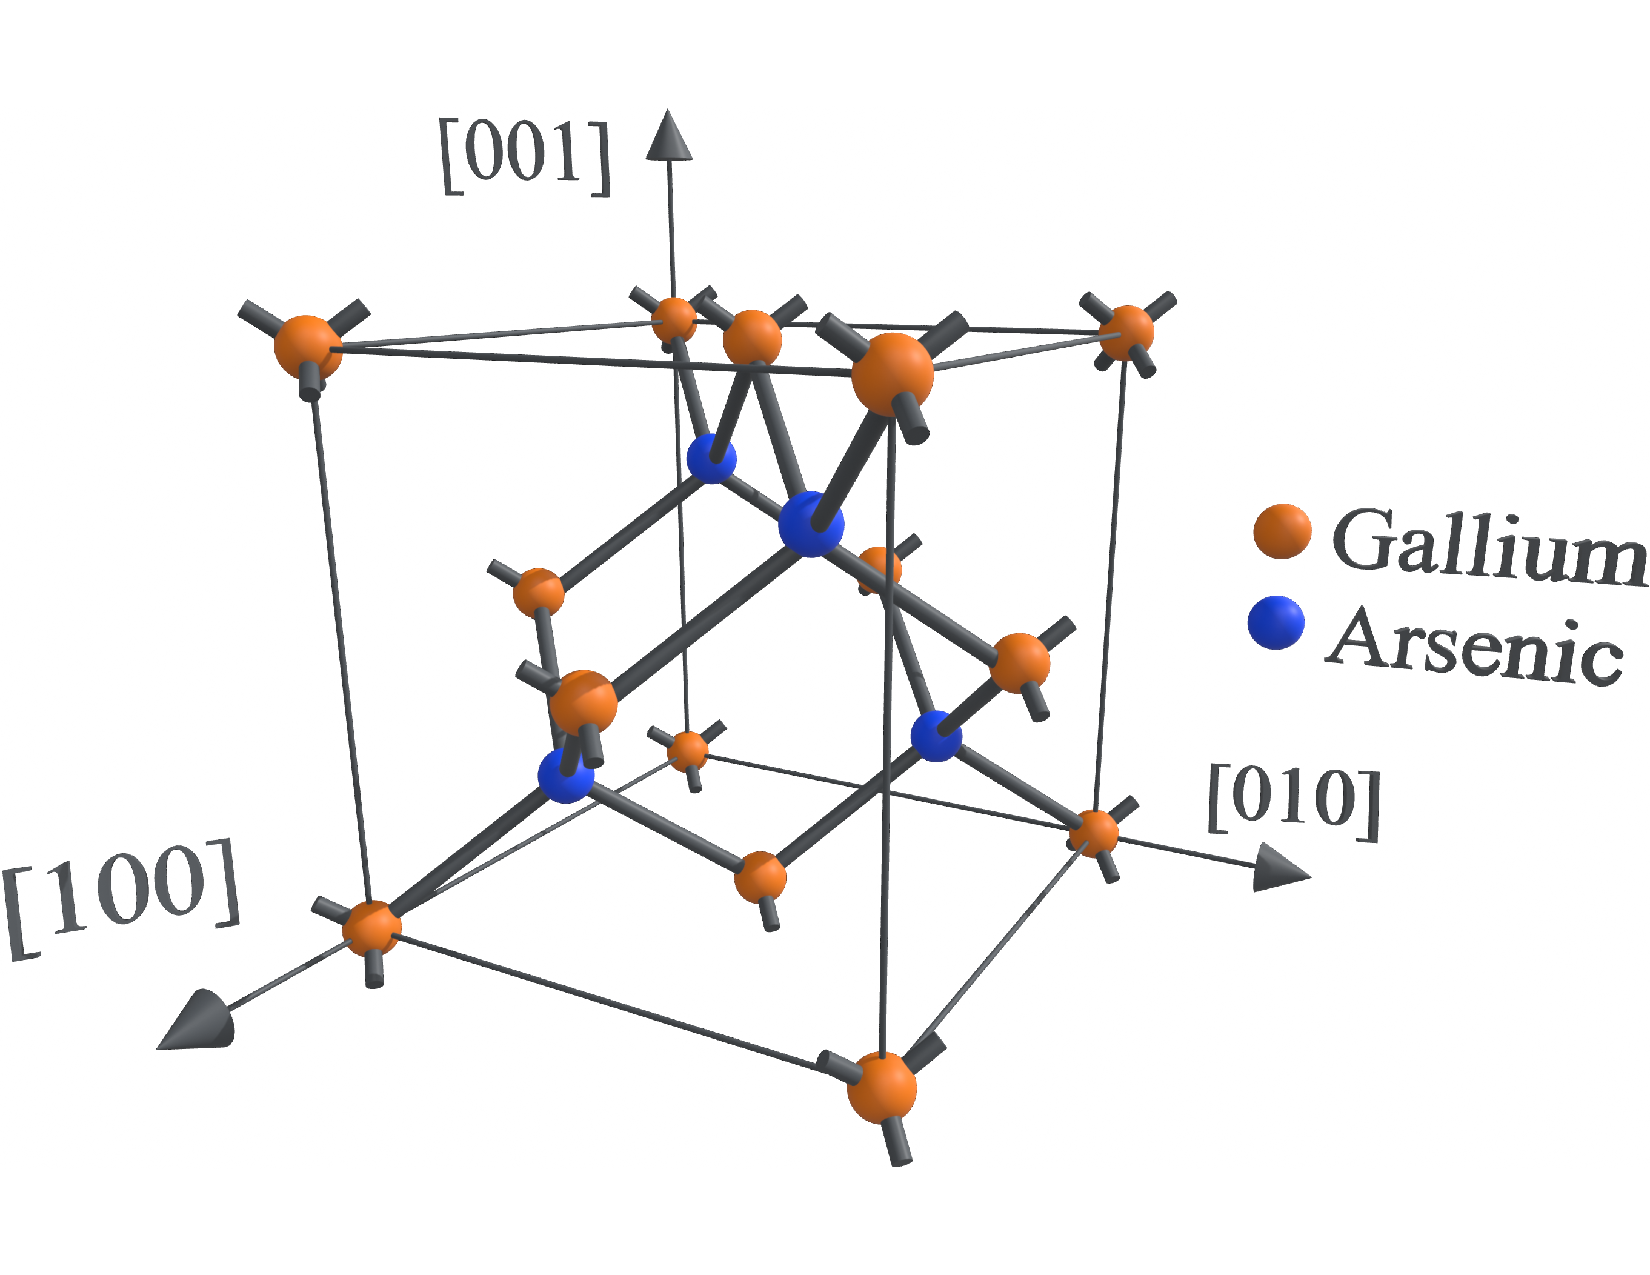
\includegraphics[width=.5\textwidth]{figs/ALGAAS/gaas_unit_cell_mi.pdf}
\caption{The unit cell of gallium arsenide (GaAs) with associated miller indices as coordinate axes}
\end{center}
\label{fig:gaas_uc}
\end{figure}

%% Mention the difference in lattice cell constant between $\gaas$ and $\algaas$?

\subsection{Induced anisotropy in zincblende crystals}
Zincblende structures, like the crystalline materials in question can exhibit birefringent properties when under influence of mechanical stresses and static / low-frequency electric fields ($E_\mathrm{STLF}$); characterized by photoelastic and electro-optic effects respectively. 

\subsubsection{The (linear) electro-optic (Pockel's) effect}

For non-centrosymmetric crystalline media there exists a non-zero rank 2, $6 \times 3$ tensor ($r_{ij}$) connecting a low-frequency \footnote{``low frequency'' meaning orders of magnitude smaller than an optical field it effects} electric field $\vec{E}(f) = [E_x(f), E_y(f), E_z(f)]$ directly to the \hyperref[sec:indicatrix]{indicatrix} ~\cite{yariv,nye}:
\begin{equation}
  \left[ {\begin{array}{c}
   \big( \frac{1}{\Delta n ^2 } \big)_1 \\
   \big( \frac{1}{\Delta n ^2 } \big)_2 \\
   \big( \frac{1}{\Delta n ^2 } \big)_3 \\
   \big( \frac{1}{\Delta n ^2 } \big)_4 \\
   \big( \frac{1}{\Delta n ^2 } \big)_5 \\
   \big( \frac{1}{\Delta n ^2 } \big)_6 \\
  \end{array} } \right]
  =
%
 \left[ {\begin{array}{ccc}
   r_{11} & r_{12} & r_{13}\\
   r_{21} & r_{22} & r_{23}\\
   r_{31} & r_{32} & r_{33}\\
   r_{41} & r_{42} & r_{43}\\
   r_{51} & r_{52} & r_{53}\\
   r_{61} & r_{62} & r_{63}\\
  \end{array}} \right]
 %
 \left[{\begin{array}{c}
   E_x (f)\\
   E_y (f)\\
   E_z (f)\\
 \end{array}} \right]
\end{equation}

\noindent The $i$ index runs over the terms in the indicatix equation:
\begin{equation}
\bigg(\frac{1}{\Delta n_x^2} \bigg) x^2\ + \bigg(\frac{1}{\Delta n_y^2} \bigg) y^2 + \bigg(\frac{1}{\Delta n_z^2} \bigg) z^2 + 2 \bigg(\frac{1}{\Delta n_{xz}} \bigg)xz + 2 \bigg(\frac{1}{\Delta n_{yz}} \bigg)yz + 2 \bigg(\frac{1}{\Delta n_{xy}} \bigg)xy = 1
\end{equation}

%%Detail on some prior knowledge of $f \leq f_\mathrm{max}$? (Pockels cell specs?)

\subsubsection{$r_{ij}$ for zincblende crystals ($r_{\bar{4}3m, ij}$)}

The form of the electro-optic tensor for zincblende crystals (including $\gaas$ and $\algaas$) reduces such that $r_{ij} = r_{41} = r_{52} = r_{62} \neq 0$ with all other terms being zero:

\begin{equation}
r_{\bar{4}3m,ij} =
 \left[ {\begin{array}{ccc}
  0 & 0 & 0\\
  0 & 0 & 0\\
  0 & 0 & 0\\
  r_{41} & 0 & 0\\
  0 & r_{52} & 0\\
  0 & 0 & r_{63}\\
 \end{array}} \right]
\end{equation}

\noindent Where also $r_{41} = r_{52} = r_{63}$

\subsubsection{New principal (electro-optic) dielectric axis for zincblende structures}

In general the principle dielectric axes of the new ellipsoid do \textbf{not} coincide with the axes of the ellipsoid of the unperturbed crystal. The form of the index ellipsoid for a zincblende crystalline material accounting for the electro-optic tensor and some generalized DC electric field $\vec{E}$ expressed in terms of the crystallographic axes is given by:
\begin{equation}\label{eq:zindicatrix}
\bigg(\frac{1}{n_o^2} \bigg) x^2\ + \bigg(\frac{1}{n_o^2} \bigg) y^2 + \bigg(\frac{1}{n_o^2} \bigg) z^2  + 2r_{41} E_{[100]} yz + 2r_{41} E_{[010]} xz + 2r_{41}E_{[001]} xy= 1
\end{equation}

\noindent Where we have set $n_x = n_y = n_z = n_o$ for zincblende structures.

\noindent Eigenvectors of the above tensor equation, produce the two principal axes:	

\begin{equation}
 \left[ {\begin{array}{ccc}
   \big( \frac{1}{n_o ^2} \big)& r_{41}E_{[001]} & r_{41} E_{[010]}\\
   r_{41}E_{[001]} & \big( \frac{1}{n_o ^2} \big) &  E_{[100]}\\
   r_{41} E_{[010]} & r_{41} E_{[100]} & \big( \frac{1}{n_o ^2} \big)\\
  \end{array}} \right]
\end{equation}

\subsubsection{The photoelastic effect}

General strains $S_{kl}(r) = \frac{1}{2} \bigg[ \frac{\partial u_k (r)}{\partial x_i} + \frac{\partial u_i (r)}{\partial x_k} \bigg]$, when applied to a material, also impact the indicatrix via the photoelastic tensor $p_{idkl}$:

\begin{equation}
 \bigg( \frac{1}{\Delta n^2} \bigg)_{ij} = p_{ijkl} S_{kl}
\end{equation}

For realistic mirror coatings, heteroepitaxial bonding between $\gaas$/$\algaas$ layers may produce an intrinsic strain within the HR stack and can lead to the existence of a static non-negligible birefringence throughout the coating layers \cite{Cole:16}.

\subsubsection{The generalized indicatrix}
Both forms of the induced birefringence (electro-optic and photo-elastic) can be incorportated into a condensed form \cite{nye}:

\begin{equation}\label{eq:indicgen}
	\bigg( \frac{1}{\Delta n^2} \bigg)_{ij} = r_{ijk}E_k + p_{ij \alpha \beta} \epsilon_{\alpha \beta}
\end{equation}

Where $\alpha$ and $\beta$ are dummy indices connecting the elasto-optic ($p_{ij \alpha \beta}$) tensor to the stress tensor ($\epsilon_{\alpha \beta}$) via stress-strain / piezoelectric relations:

\begin{equation}\label{eq:indicgen_stress2strain}
	\epsilon_{ij} = r_{kij}E_{k} + s_{ijkl} \sigma_{kl}
\end{equation}
\begin{equation}\label{eq:indicgen_elasto_optical}
 \begin{split}
	p_{ij \alpha \beta} = \pi_{ijkl} C_{kl \alpha \beta}
	\\
	\pi_{ijkl} = p_{ij \alpha \beta} s_{ijkl}
 \end{split}
\end{equation}

%%New principal dielectric axes for zincblende structures (zinblende photoelastic tensor, zincblende electro-optic tensor)

\subsection{EO Modulation}\label{sec:EOM}
Imparting phase modulations onto an optical carrier field is a common application of the electro-optic effect. Electro-optic modulators (EOMs) or Pockel cells are sold as a standard optical components usually composed of a monolithic crystalline material sandwiched between two capacitor plates connected to a single electrical input port (typically coaxial) designed to take in a voltage input of frequency ($\Omega$) within a specified modulation amplitude and frequency bandwidth. When the field amplitude across the crystal is driven by a voltage controlled oscillation, the coefficients within the electro-optic tensor vary linearly. The voltage amplitude of the signal input is proportional to the strength of the phase modulation on the optical carrier field of frequency ($\omega$) and is commonly quantified in terms of a modulation index ($\beta$).

%%Consider a specific crystal that gives us our $\beta \mathrm{sin}(\Omega t)$

\begin{equation}\label{eq:inp_EOM}
E_\mathrm{out} = E_o e^{i \omega t + \beta \mathrm{sin}( \Omega t)} \approx
\end{equation}

\begin{figure}[!ht]
\begin{center}
	\begin{subcaptiongroup}
	     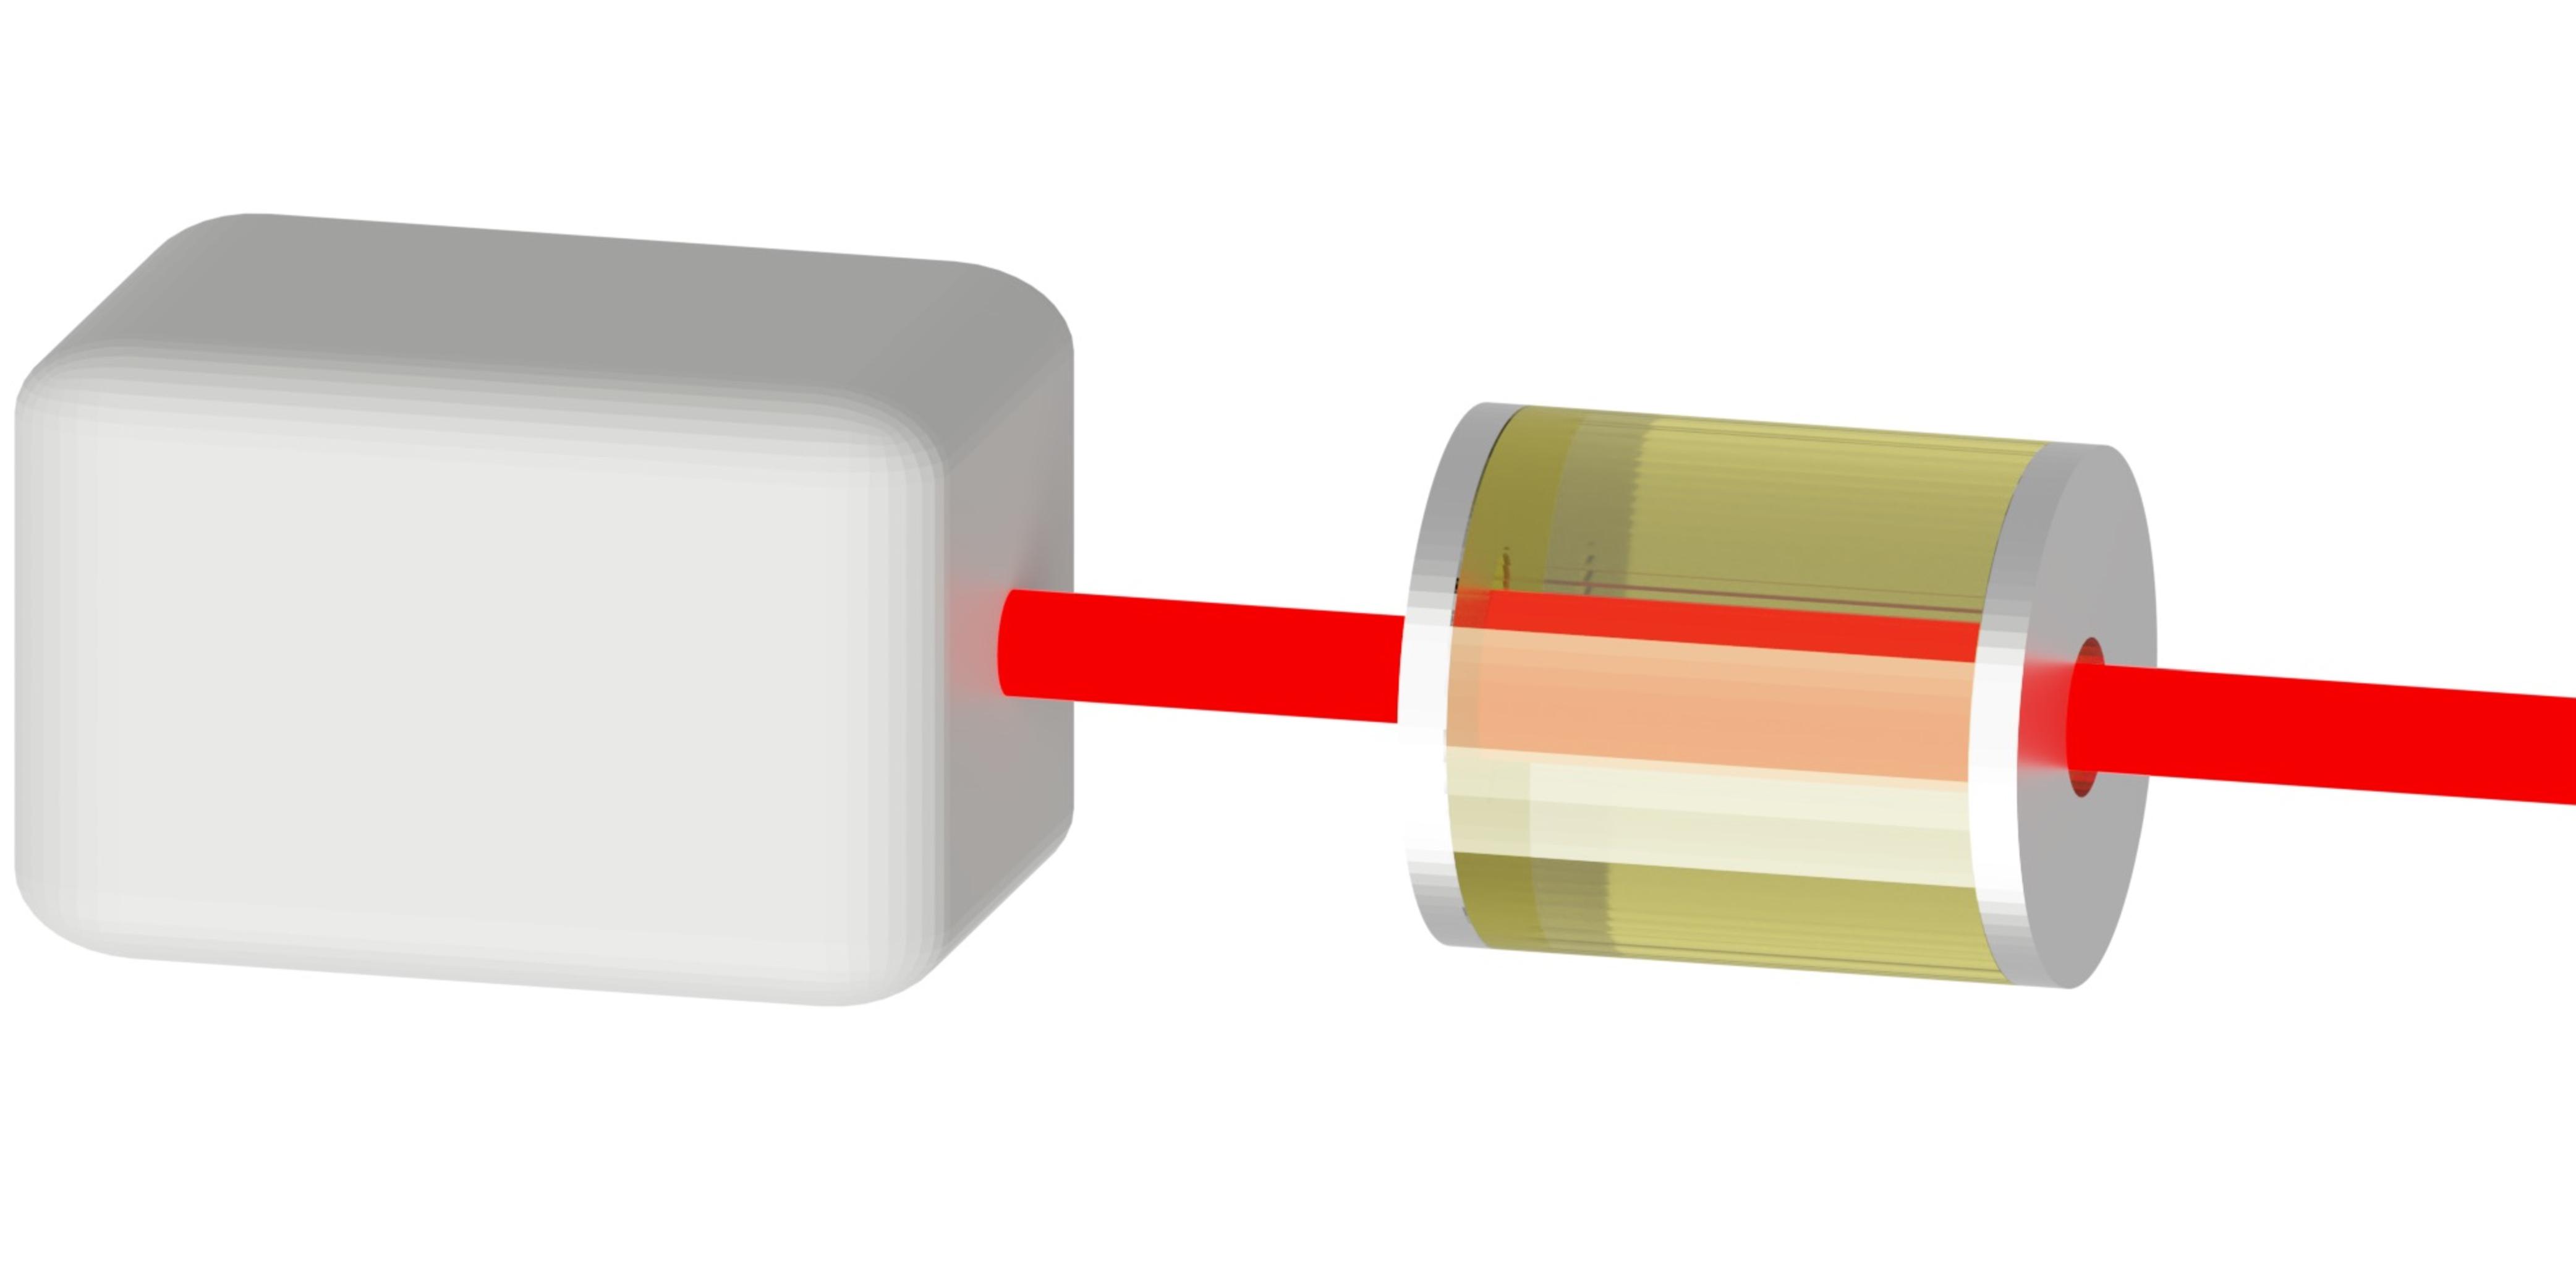
\includegraphics[width=.6\textwidth]{figs/ALGAAS/eom_l_assembly.pdf}
	     \phantomcaption\label{pc_longitudinal}
	     \\
	     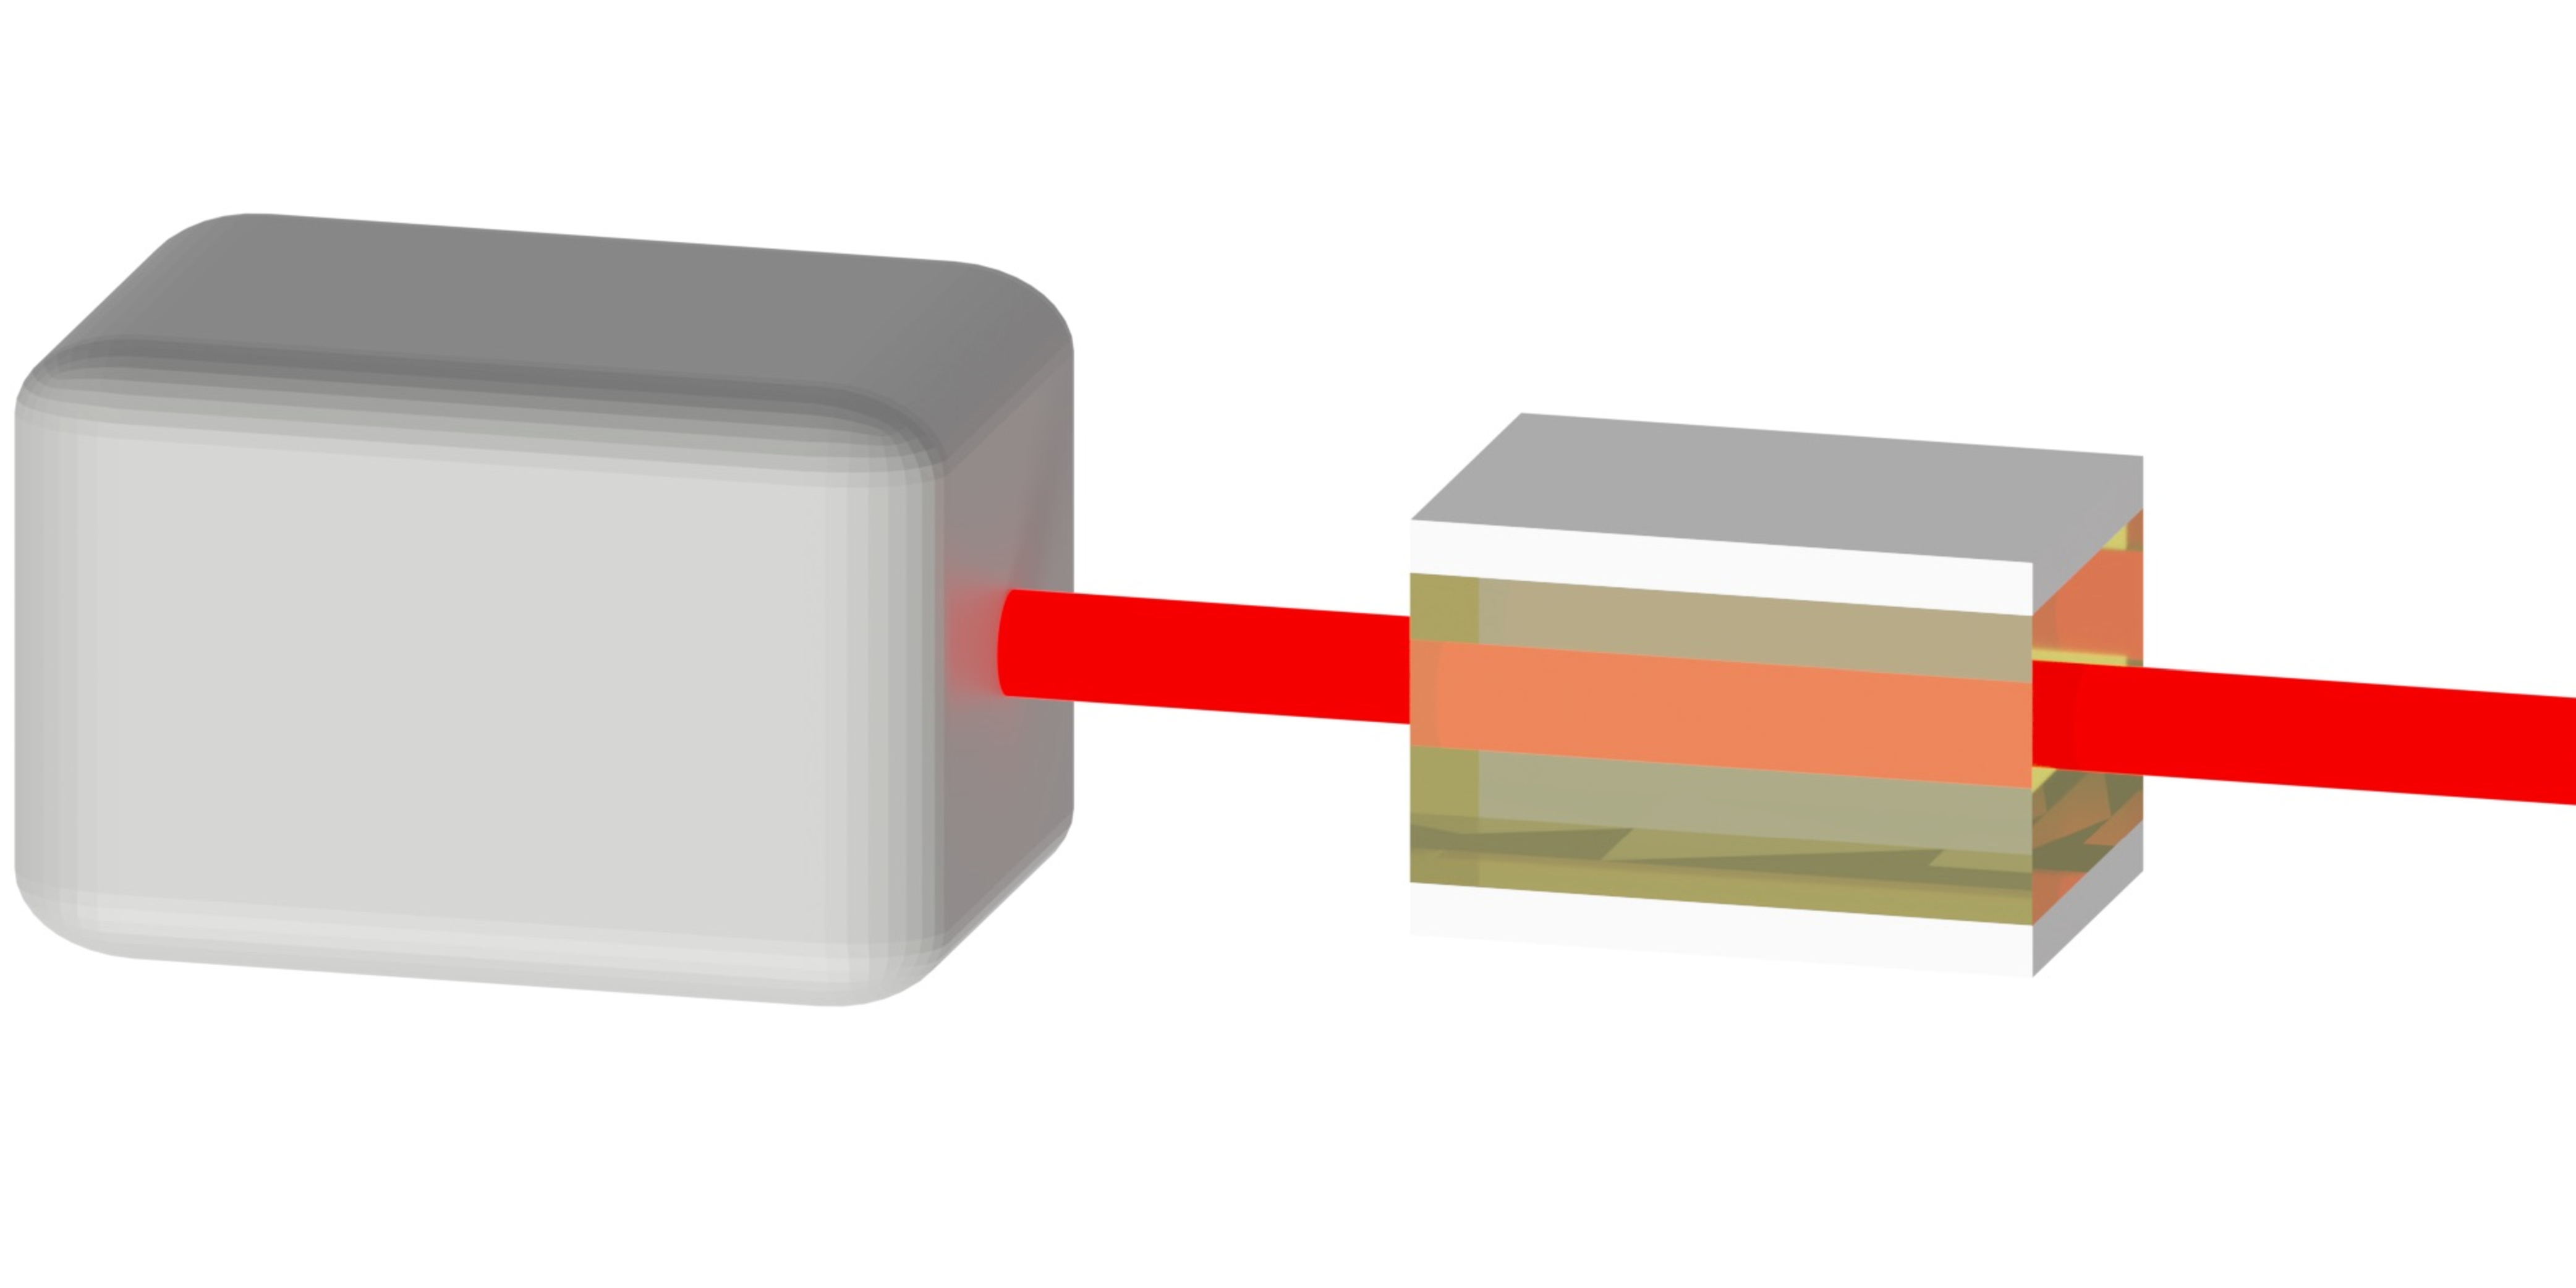
\includegraphics[width=.6\textwidth]{figs/ALGAAS/eom_t_assembly.pdf}
	     \phantomcaption\label{pc_transverse}
	\end{subcaptiongroup}
\end{center}
    \caption{Longitudinal and Transverse Pockels cells}
    \label{fig:lpc_and_tpc}
\end{figure} 


Bessel function approximations sufficiently demonstrate that the phase modulated carrier field imparts power to optical sideband fields separated in frequncy by an integer multiple of the modulation $n \cdot \Omega$. Typically $\Omega$ is a chosen frequency used for optical heterodyne detection; while for noise-driven modulation, the phase coupling shows strong coorelation to the relevant E-field spectra alongside the length of the beam propogation within the electro-optic media.

\subsection{Optical anisotropy of a HR $\gaas$ / $\algaas$ stack}
A comprehensive review of the relevant birefringent properties of a HR $\gaas$/$\algaas$ mirrorstack is due, and for this body of work includes: 1) crystal coordinate considerations when asserting an optical axis on a highly reflective crystalline stack manufactured by the Thorlabs crystalline coatings division, 2) citations of coating parameters and observed intrinsic birefringence from the highly reflective coating stack in question, 3) analysis of the differential electro-optic effect on the phase of a reflected beam, and 4) estimating the the differential phase noise in LIGO based on preliminary electric field measurements measured at LHO.

\begin{figure}[!ht]
    \begin{subcaptiongroup}
	    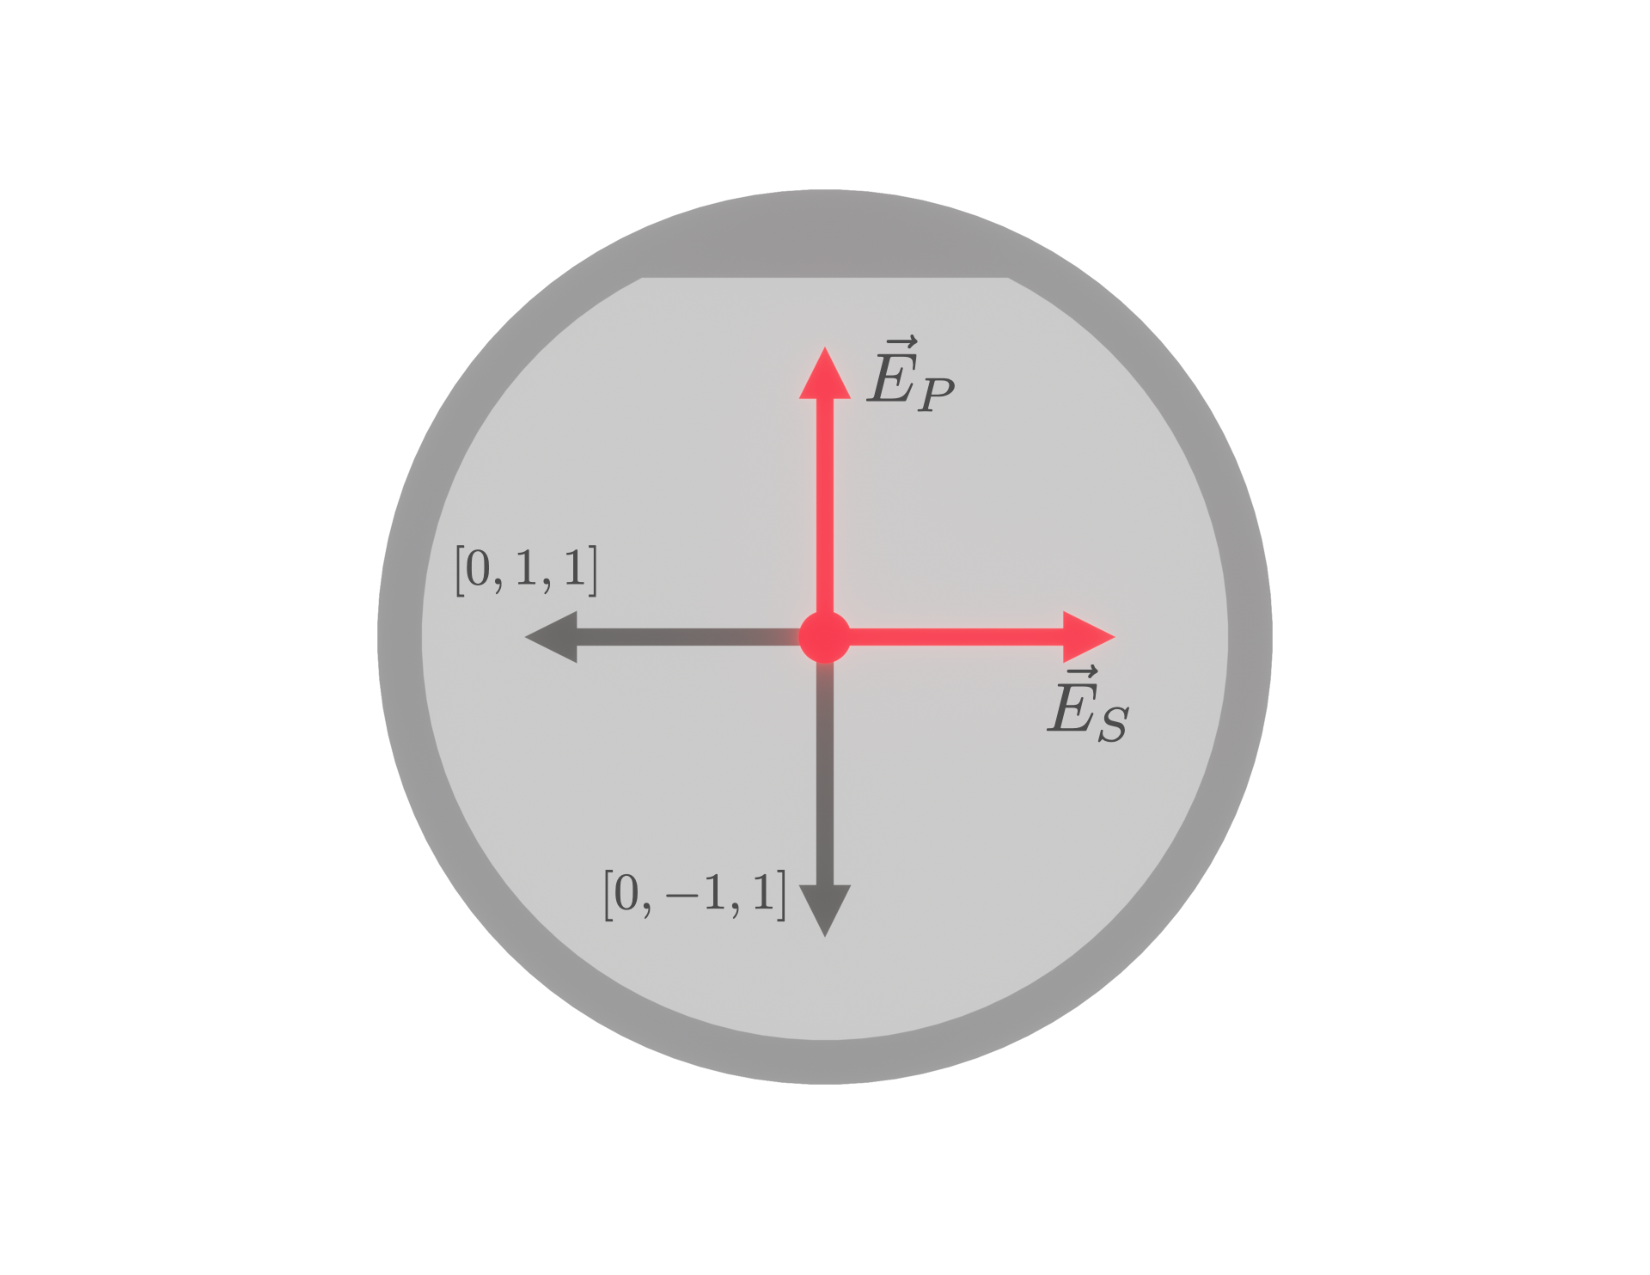
\includegraphics[width=.5\textwidth]{figs/ALGAAS/coating_orientation_normal.pdf}
	    \phantomcaption\label{co_normal}
	    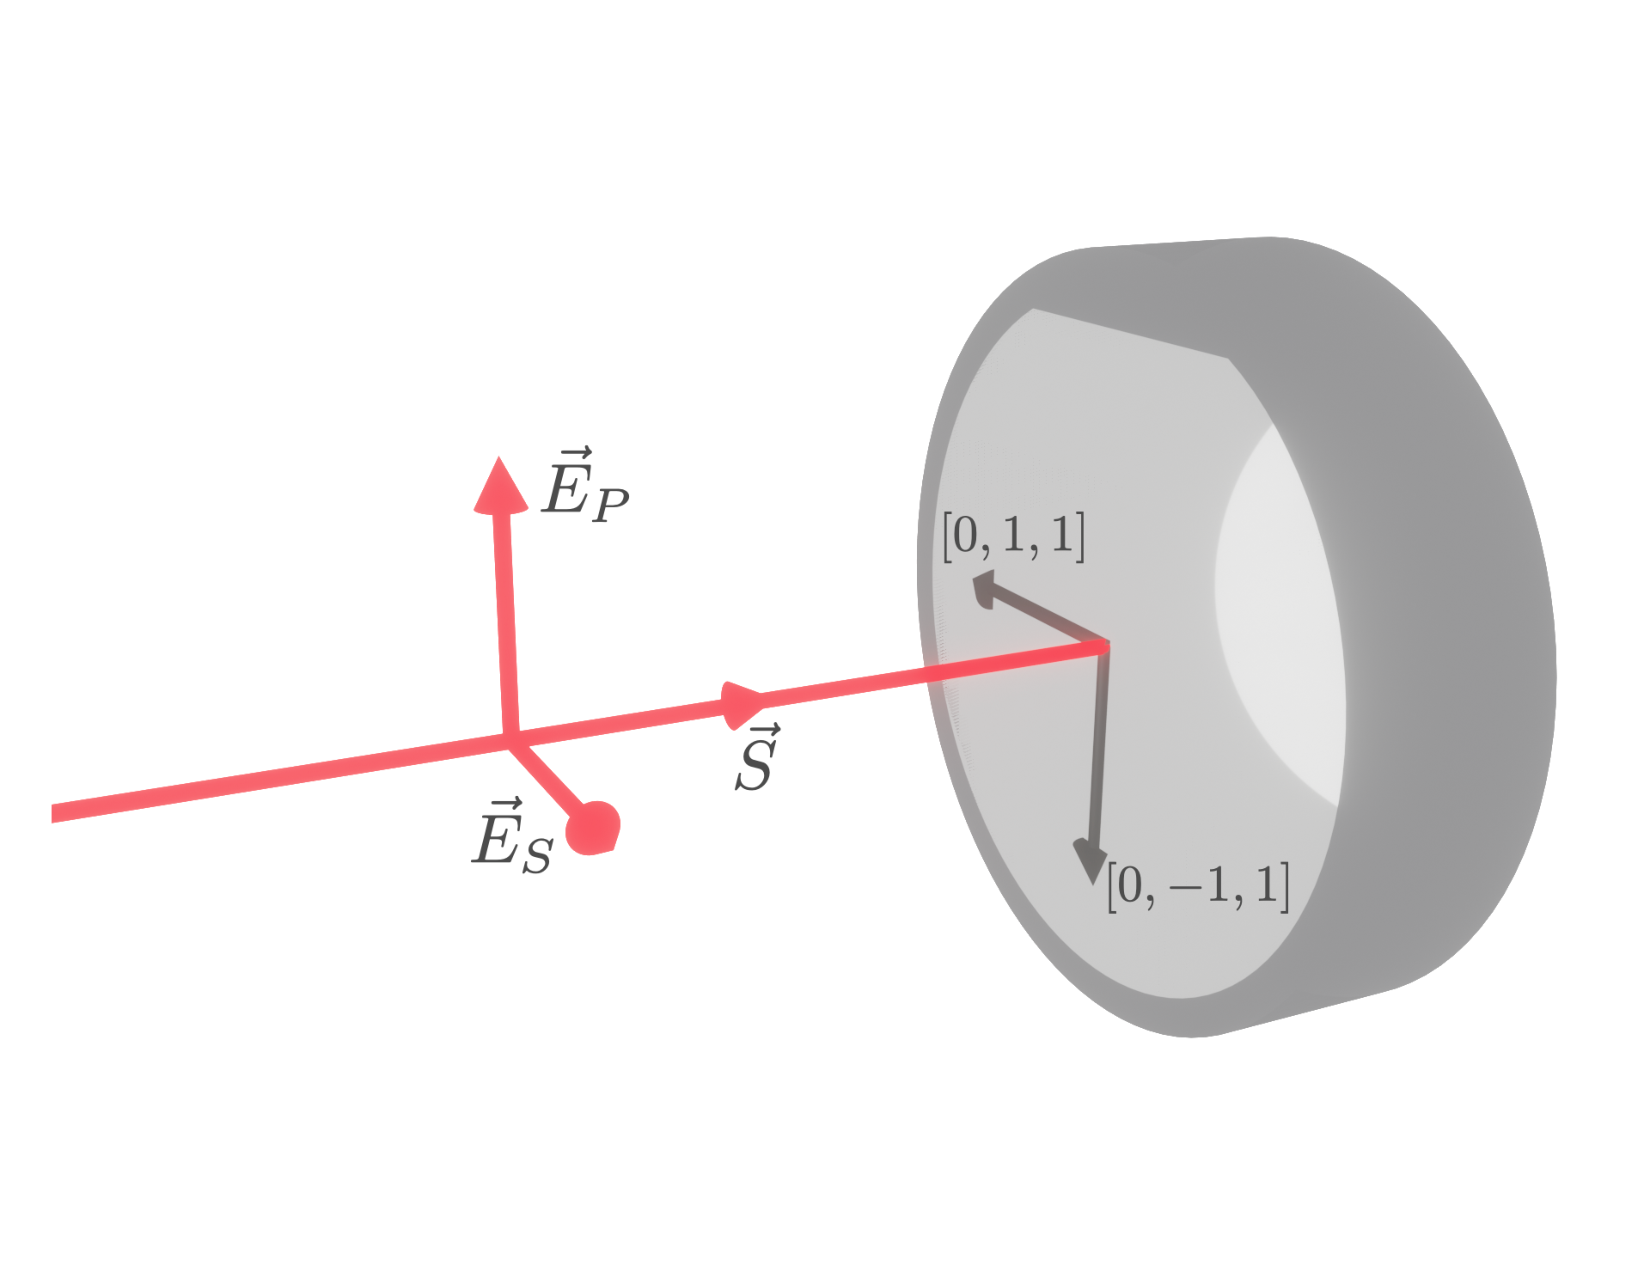
\includegraphics[width=.5\textwidth]{figs/ALGAAS/coating_orientation_isometric.pdf}
	    \phantomcaption\label{co_iso}
    \end{subcaptiongroup}
\caption{The beam propogation axis ($\vec{S}$, $[-100]$) with respect to the AlGaAs/GaAs crystal axes. The axis formed by the [100] plane normal is drawn parallel with the beam axis (z-axis) and the polarizations of incident and reflected beam oscillate along vectors within the plane formed by the normal of that axis. The AlGaAs coating is grown with a flat indicating a line within the [0-11] plane; where the plane normal points towards the sample center.}
\label{fig:algaas_coords}
\end{figure}

\subsubsection{Miller indices for highly reflective coatings $\gaas$/$\algaas$ coatings}
Up to this point three varieties of orthonormal coordinates are addressed: the crystal axis (as indicated by Miller index plane normals), the principal dielectric axis (based on diagonalization of the indicatrix), and an optical beam axis (when considering a desired (laser) light propogation). The asserted beam axis is cited \ref{fig:algaas_coords}.

\subsubsection{Electro-optic coupling to the reflected phase of a HR mirror coating}
With our chosen beam axis, the influence of an isotropic white noise field ($E_n = [E_{nx},E_{ny},E_{nz}]$) is considered:

\begin{equation}
 \left[ {\begin{array}{ccc}
   \big( \frac{1}{n_o ^2} \big)& r_{41}E_{ny} & r_{41} E_{nx}\\
   r_{41}E_{ny} & \big( \frac{1}{n_o ^2} \big) & r_{41} E_{nz}\\
   r_{41} E_{nx} & r_{41} E_{ny} & \big( \frac{1}{n_o ^2} \big)\\
  \end{array}} \right]
\end{equation}

Assuming $E_n$ is small, the indicatrix change of $E_{nx}$ and $E_{ny}$ relative to $E_{nz}$ (as seen by the beam polarization) will be small ($r_{41}E_{n(x/y)} \ll r_{41}E_{nz}$). After diagonalizing with relevant terms \footnote{Note that the form of the tensor is still in the crystal coordinates but the $E_n$ terms are placed in the tensor such that their directions align with beam axis coordinates.} in the tensor, we are left with the following eigenindices:

\begin{equation}
\begin{aligned}
n_x' & = n_o - r_{41}E_{nz} \\
n_y' & = n_o + r_{41}E_{nz}
\end{aligned}
\end{equation}

%How the modulation of the phase of the carrier field is dependent on the orientation of its wave vector with respect to the crystal structure, the modulating electric field direction and strength, (other items to discuss in terms of introducing the effect)
%% For GaAs @ $10.6\mu$ $r_{41} = 1.6 \times 10^{-12}$ [m/V]
%% Adachi estimate for $\mathrm{Al_{x}Ga_{1-x}As}$?
%% Relevant eigenpolarizations, non-optical field $E_y = E_z = 0$?}
%% FIGURE: SUB1 Transformed indicatrix (Before and after $E_x$)
%% FIGURE: SUB2 Ellipse cross section. New eigenpolarizations and corresponding indices and their influence on incident field (Marty's result)

Assuming we are operating in a coordinate system suggested in \hyperref[fig:algaas_coords]{Figure 3.4}, which plane is impacted by some $E_\mathrm{noise}$? Revisiting the \hyperref[eq:zindicatrix]{indicatrix} we can see that for even non-zero z and y components that the only coupling to the input beam polarization is the index along the cross coupled zy-axis through $E_z$ is that of the $E_x$ term. This gives us the ability to easily diagonalize the indicatrix tensor by setting non-relevant field terms to zero.
Fejer and Bonilla take an analytical approximation approach when finding the impact of the electric field to the change in phase of the light through a crystalline anisotropic thin film ($\lambda/4$) stack \cite{bonillafejer}.

\begin{equation}
\hat{\phi}' = \frac{\pi n_1 z}{1-z^2}(z^{2N} -1) \frac{z^{2N} \frac{(n_f)^2}{n_2 n_3}(n_2 \kappa_{\gamma 2} + n_3\kappa_{\gamma 3}) - (n_2 \kappa_{\gamma 3} + n_3\kappa_{\gamma 3})}{(n_1)^2 -(n_f)^2 z^{4N}}
\end{equation}

with $z = \frac{n_2}{n_3}$
and
$
\kappa_{\gamma j} = \frac{d}{d \gamma} \mathrm{log}(n_j h_j)|_{\gamma =\gamma_{O}} \bigg(\frac{\hat{n}_j'}{\hat{n}_j} +\frac{\hat{h}_j'}{\hat{h}_j} \bigg)
$

With $\kappa$ being a scalar parameter.
%%FIGURE: Cross sectional view of multilayer coating

\begin{figure}[!ht]
    \begin{subcaptiongroup}
	    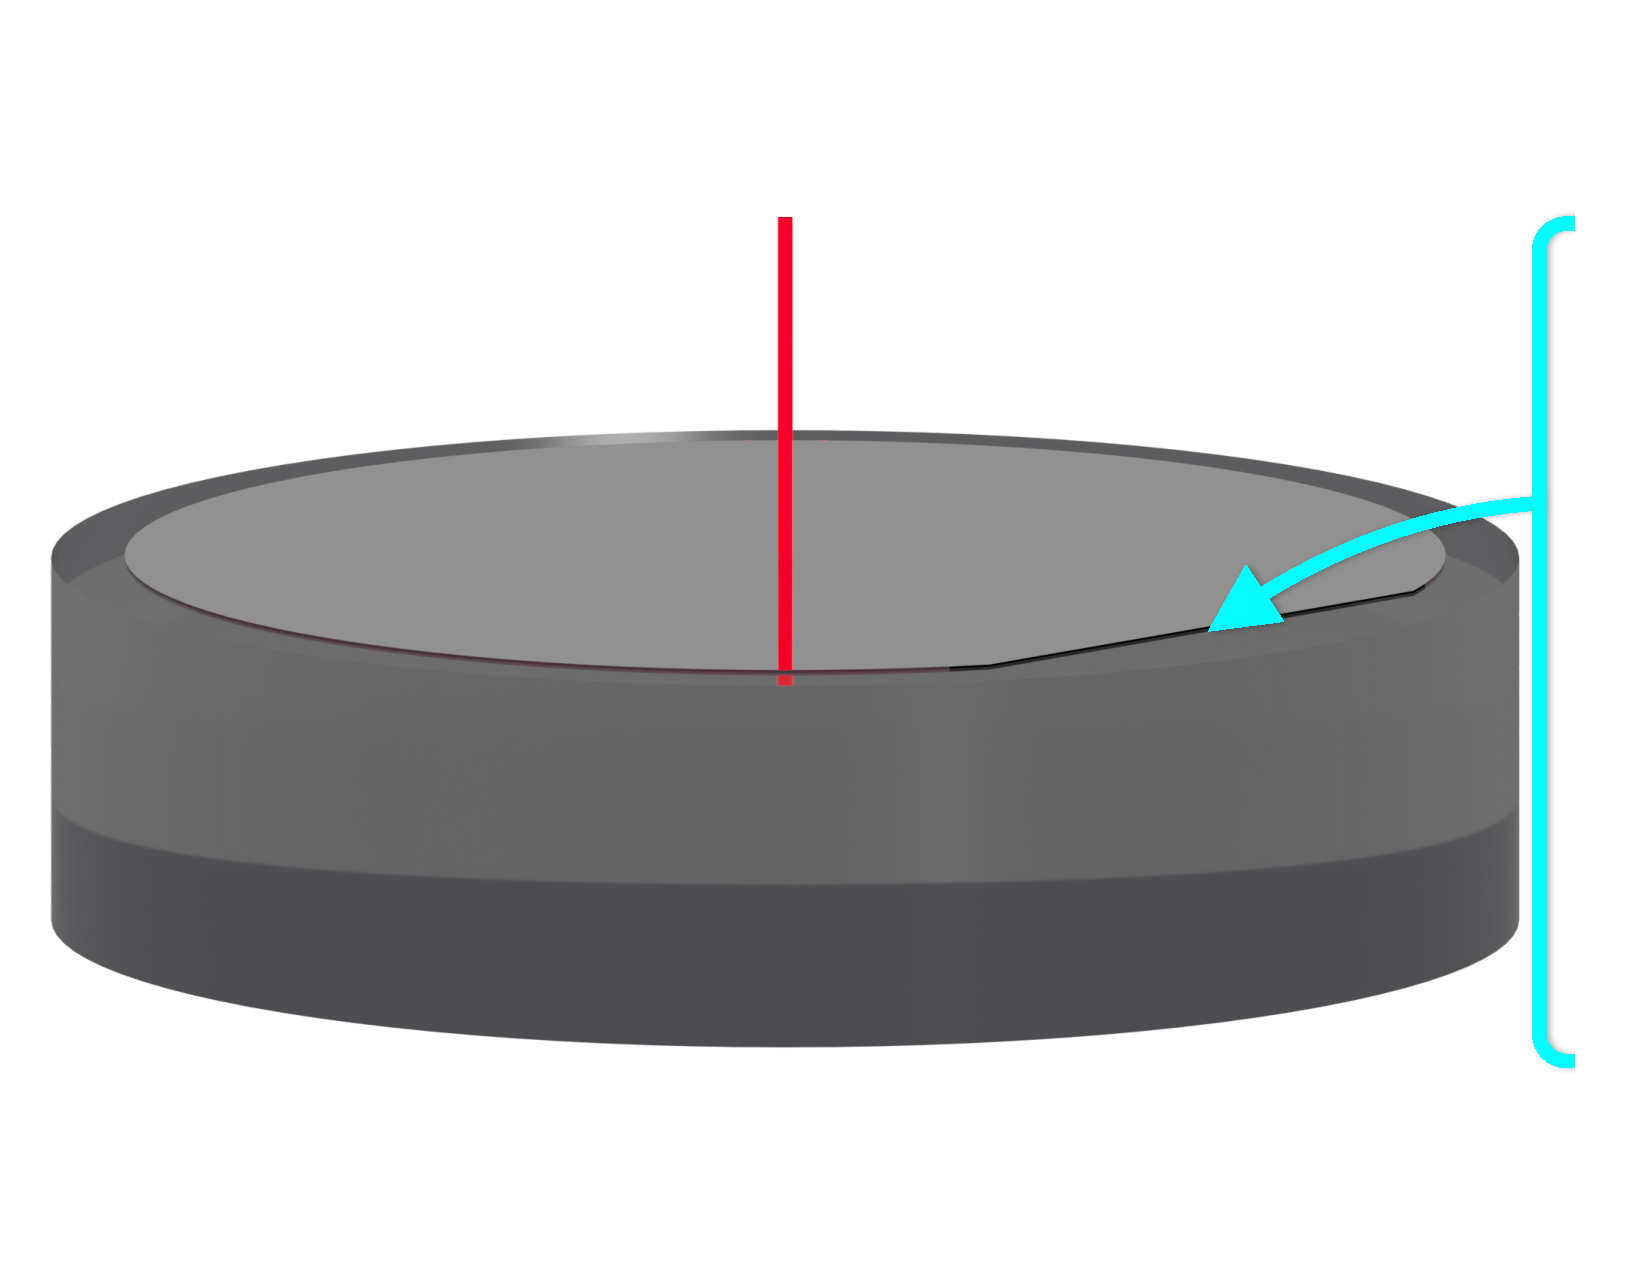
\includegraphics[width=.55\textwidth,page=1]{figs/ALGAAS/ALGAAS_HR_layers_1.pdf}
	    \phantomcaption\label{HRiso}
	    \includegraphics[width=.55\textwidth,page=2]{figs/ALGAAS/ALGAAS_HR_layers_1.pdf}
	    \phantomcaption\label{HRxsection}
    \end{subcaptiongroup}
\caption{The beam propogation axis ($\vec{S}$, $[-100]$) with respect to the AlGaAs/GaAs crystal axes. The axis formed by the [100] plane normal is drawn parallel with the beam axis (z-axis) and the polarizations of incident and reflected beam oscillate along vectors within the plane formed by the normal of that axis. The AlGaAs coating is grown with a flat indicating a line within the [0-11] plane; where the plane normal points towards the sample center.}
\label{fig:HRlayers}
\end{figure}


\subsubsection{Numerical estimate}

In the appendix of \cite{ballmer2015} Ballmer constructs a coating layer transfer function for a given coating layer k with index $n_k$, and thickness $d_k$, defining right and left propogating modes $\Psi^{R,L}$ repsectively:

\begin{equation}
  \left[ {\begin{array}{c}
   \Psi^\mathrm{R} \\
   \Psi^\mathrm{L} \\
  \end{array} } \right]_{k+1}
  =
%
Q_k D_k
%
 \left[{\begin{array}{c}
   \Psi^\mathrm{R} \\
   \Psi^\mathrm{L} \\
 \end{array}} \right]
\end{equation}

\noindent $D_k$ applies the phase ($\phi_k = 4\pi n_k d_k /\lambda_0$) from a given coating layer, and $Q_k$ applies the transfer function between high-low/low-high index layers transition:

\begin{equation}
Q_k = \frac{1}{2n_{k+1}}
\left[ {\begin{array}{cc}
  n_{k+1} + n_k & n_{k+1} - n_k\\
 n_{k+1} - n_k & n_{k+1} + n_k\\
\end{array} } \right]
\end{equation}

\begin{equation}
D_k =
\left[ {\begin{array}{cc}
  e^{-i \phi_k / 2}& 0\\
 0 & e^{i \phi_k / 2}\\
\end{array} } \right]
\end{equation}
Defining a HR coating stack, the total transfer matrix from vaccum $Q_0$ to the $N$th coating layer is:
\begin{equation}
M = Q_N D_N ...Q_kD_k...Q_1D_1Q_0
\end{equation}
The impact of a differential electric noise field ($E$) on $M$ due to the electro-optic effect on the kth layer, we use the chain rule:

The coating to be studied consists of 36 $\lambda$/4  thick layers of $\gaas$ interspersed with 35 layers of $\lambda$/4 thick $\algaas$. $\gaas$ forms the top and bottom layer to prevent oxygen absorption from the AlGaAs layer. The $\gaas$ layers have an index of $n_{\gaas} = 3.480$ and a thickness of $\Delta d_{\gaas} = 76.43$ nm while the low index $\algaas$ layers are $n_{\algaas} = 2.977$ with thickness $\Delta d_{\algaas} = 89.35$ nm. With the cosntructed matrices, we apply these parameters and compute a differential phase of:

%High Index:  GaAs, n=3.480, layer thickness is 76.43 nm
%Low Index:  $ \mathrm{Al}_{0.92} \mathrm{Ga}_{0.08} \mathrm{As} $, n=2.977, layer thickness is 89.35 nm
%Info from Steve. Written source


\subsection{Measured birefringence from HR $\gaas$/$\algaas$ mirrors}

There are different accounts of a measured birefringence from HR $\gaas$ / $\algaas$ (\href{https://dcc.ligo.org/DocDB/0181/G2200386/001/G2200386.pdf}{Satoshi}, \href{https://nodus.ligo.caltech.edu:8081/CTN/1474}{CTN}, \href{https://dcc.ligo.org/DocDB/0181/G2200559/001/G2200559-v1%20-%20polarization.pdf}{Aidan})

%%Is the measured birefringence static? (Layer bonding method might introduce something?)
%% Does it change from different mounting methods? (Photoelastic) (order of magnitude estimate)
%% Electro-optic ruled out based on field measurements and relative coupling factor.
%% Measurement precision of the coating birefringence? Cavity length, Polarization drifts, etc.

The measured birefringence is estimated to be caused by an intrinsic strain between the epitaxial layers of $\gaas$/$\algaas$. \cite{Cole:2013}

%% Marty's document about Birefringence in Crystalline mirror coatings V.8

\section{Projected DARM coupling (initial)}
To estimate how much DARM coupling can occur, we use use a measured field spectra acquired from installed electric field meters located within LIGO Hanford Observatory ETMX and ETMY vacuum chambers. Taking the upper and the lower EFM measurements in $.3\; [\mathrm{V}/\mathrm{m}/\sqrt{\mathrm{Hz}]}$ @ 60 Hz and $4\times10^{-3}\; [\mathrm{V}/\mathrm{m}/\sqrt{\mathrm{Hz}]}$ @ 4kHz ~\cite{efmlog}.
%% \satoshi{I don't think these values are calibrated. According to Martynov et al. 2016, the fluctuations in the electric filed is $\sim10^{-5}\,\mathrm{[(V/m)/\sqrt{Hz}]}$.}
This along with computed estimate allows us to create an upper limit for what this noise might be assuming incoherent fields between the end stations and a flat frequency response within LIGO's bandwidth.
%%FIGURE: GWINC noise against calibrated electro-optic noise estimate. Full bandwidth

\section{A Short in-air FPC test}
 In seeking a calibrated estimate of the electro-optic effect for the $\gaas$/$\algaas$ mirror coating stack, we sought to measure a driven response of a mirror sample from Thorlab's crystalline mirror coatings division placed within a custom longitudinal Pockels cell mirror mount and monitored with a Pound-Drever-Hall servo. The servo was used to maintain resonance of a circulating Nd:YAG 1064nm carrier beam within an in-air two mirror Fabry-Perot cavity, with the notable mirror coating sample installed within the longitudinal Pockels cell mount and assumed the end mirror position within an in-air two mirror Fabry Perot cavity. As seen in the prior section, the size of the imparted phase noise for currently existing gravitational wave detector configurations is estimated to be small but notable. Investigation through measurement of said effect requires detection methods with sufficient sensitivity for the differential phase noise imparted by the effect. Details and specifications of the detection schema are discussed along with relevant measurements and results. 

%% Driven acoustic modes of the longitudinal pockels cell mirror mounts lead to numerous mounting strategies that will be detailed below. 
\begin{figure}[H]
	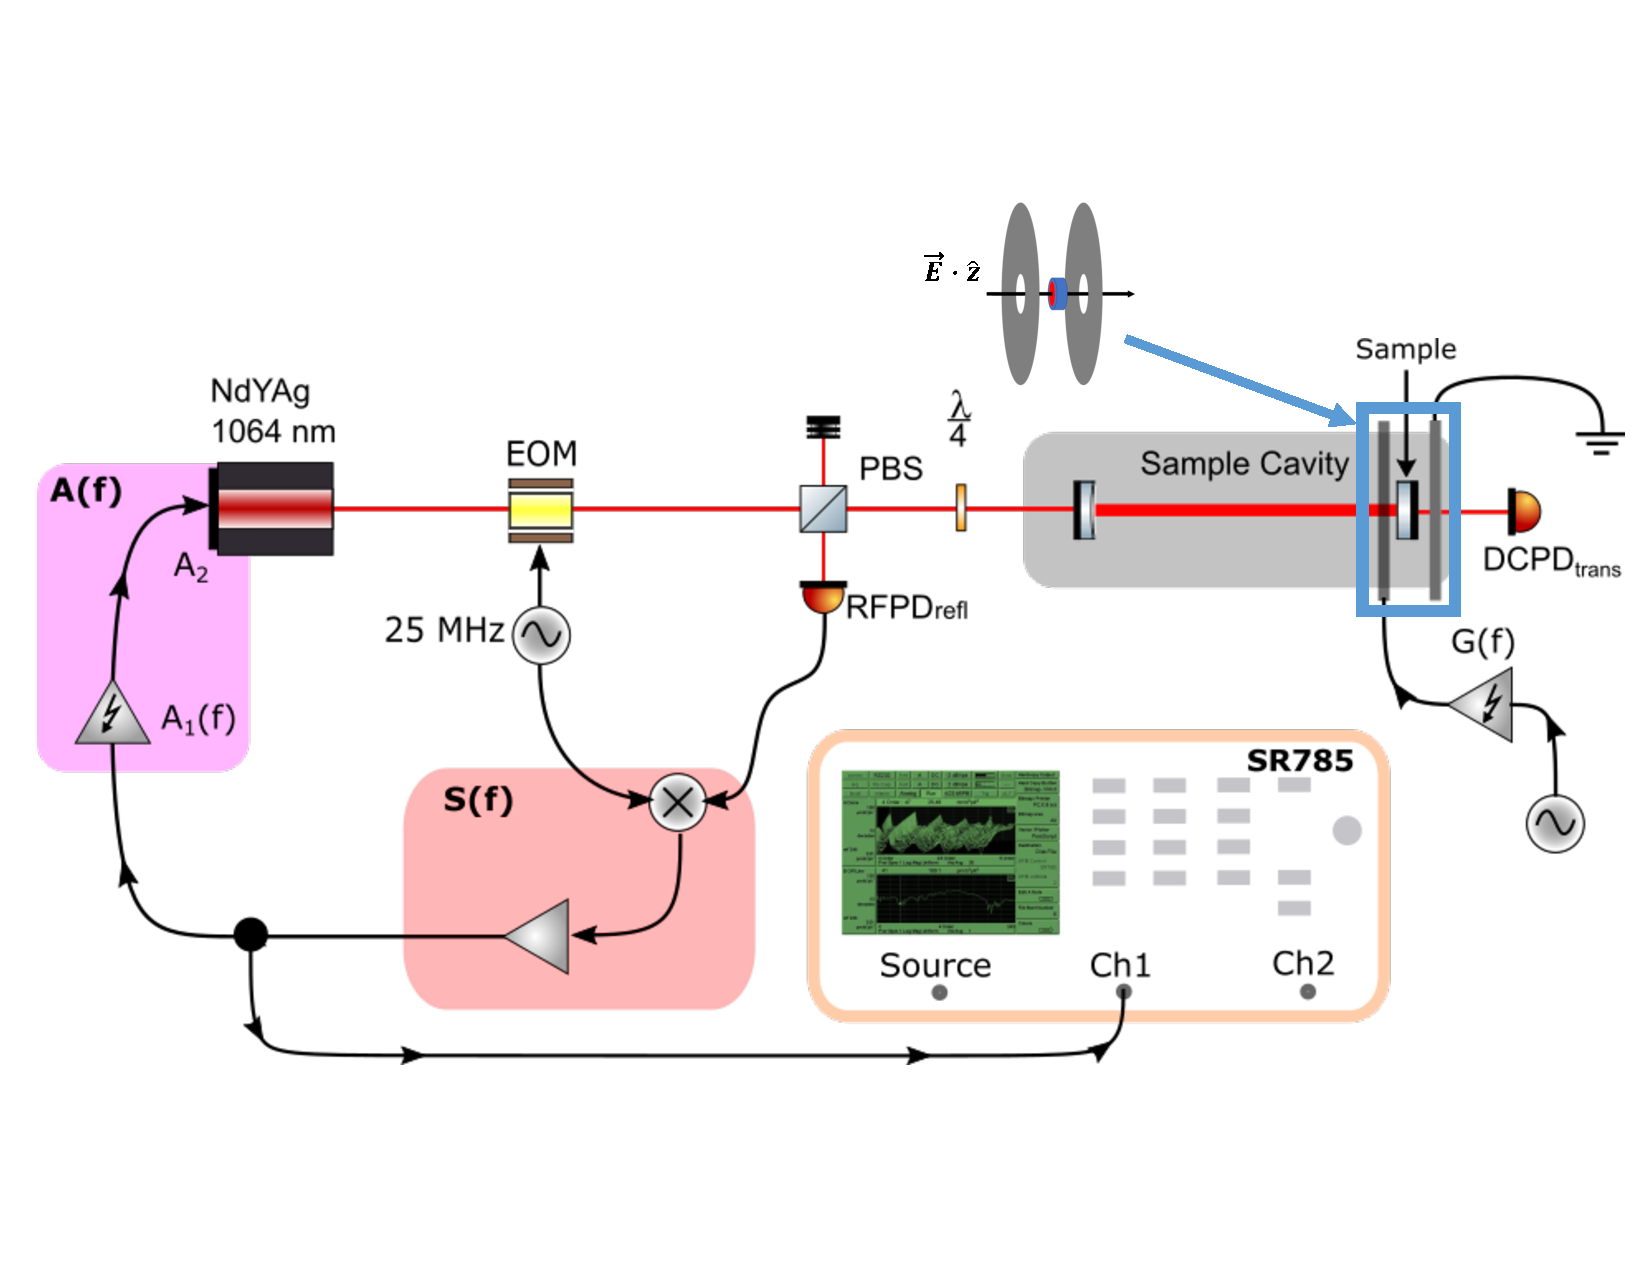
\includegraphics[width=\textwidth]{figs/ALGAAS/algaas_pockels_effect_measurement_schematic.pdf}
	\caption{A simplified and modular schematic of the PDH servo used along with an electrostatic drive mount design comprised of a disk capacitor sandwiching the HR AlGaAs sample, a high voltage amplifier, and a signal / network analyzer.}
\label{fig:simplified_experiment_schema}
\end{figure}
 Measurability of the electro-optic effect is contingent upon two initial design criteria: the sensitivity of the optical plant to be implemented in the PDH servo, and the maximum achievable electric field strength along the beam axis ($|E_z|_\mathrm{max}$).

\subsection{PDH servo}\label{subsubsec:pdh}
The Pound-Drever-Hall technique, originally and commonly used for laser frequency stabilization to an ultra-stable length reference, allows the tracking of the linear phase response of an input carrier field through cavity resonance. The servo fully realizes the ability of an optical cavity to act as a length / frequency discriminator. The alternative cavity offset lock provides a linear response in intensity, which is adequate for some applications but with reduced sensitivity due to the required power reduction by operating off resonance.
The phase measurement is extracted through an optical heterodyne; the co-propogation of a separate (but phase-locked) optical field with a known frequency separation to the carrier reflected from the cavity input. The PDH servo avoids complicated phase-locked two laser configurations, by imposing a phase modulation onto the carrier field via an electro-optic modulator (aka Pockels cell) mentioned in section \ref{sec:EOM}. If the modulation depth given by \ref{eq:inp_EOM} is set such that $\beta < 1$ then the input field may be approximated in terms of the first two Bessel functions $J_0$, $J_1$:

\begin{equation} \label{eq:EOM_trans_field}
E_\mathrm{inp} \approx E_0 [J_0(\beta)e^{i \omega t} + J_1(\beta)e^{i (\omega + \Omega) t} - J_1(\beta)e^{i(\omega -\Omega)t}]
\end{equation}

With a high enough modulation frequency the terms given above can be far enough from the carrier frequency, so that the phase modulation onto the carrier field is mathematically and physically equivalent to imposing separate optical fields (sidebands) which in most cases do not resonate in the optical cavity of interest. Setting a photodiode of area ($A_\mathrm{PD}$) in reflection of the cavity with a coefficient of $r_\mathrm{cav}(\omega,L)$, we measure the reflected power of the input field given by \ref{eq:EOM_trans_field}:

\begin{equation}
 \begin{alignedat}{3}
    &P_\mathrm{refl} && \approx \frac{|E_\mathrm{refl}|^2}{A_\mathrm{PD}} && \\
    & &&\approx \frac{E_0^2}{A_\mathrm{PD}} && \bigg\{J_0^2 |r_\mathrm{cav}(\omega,L)|^2 + J_1^2(\beta)|r_\mathrm{cav}(\omega+\Omega,L)|^2 - J_1^2(\beta)|r_\mathrm{cav}(\omega-\Omega,L)|^2 +  \\
    & && && J_0J_1(\beta)\big[r_\mathrm{cav}\omega,L) r_\mathrm{cav}^*(\omega+\Omega,L)\big] - J_ 0J_1(\beta)\big[r_\mathrm{cav}(\omega,L)r_\mathrm{cav}^*(\omega-\Omega,L)\big]\bigg\}
  \end{alignedat}
\end{equation}

The two trailing terms in the above equation for $P_\mathrm{refl}$ generate a beat frequency term between the carrier and lower and upper sidebands. The magnitude and sign of these beat terms directly relate to the phase of the reflected carrier field and can be measured and transformed to the error signal seen in \ref{fig:pdh_error} using resonant electronics (tuned to a chosen sideband frequency) for amplification and a mixer for demodulation.

\begin{figure}[H]
	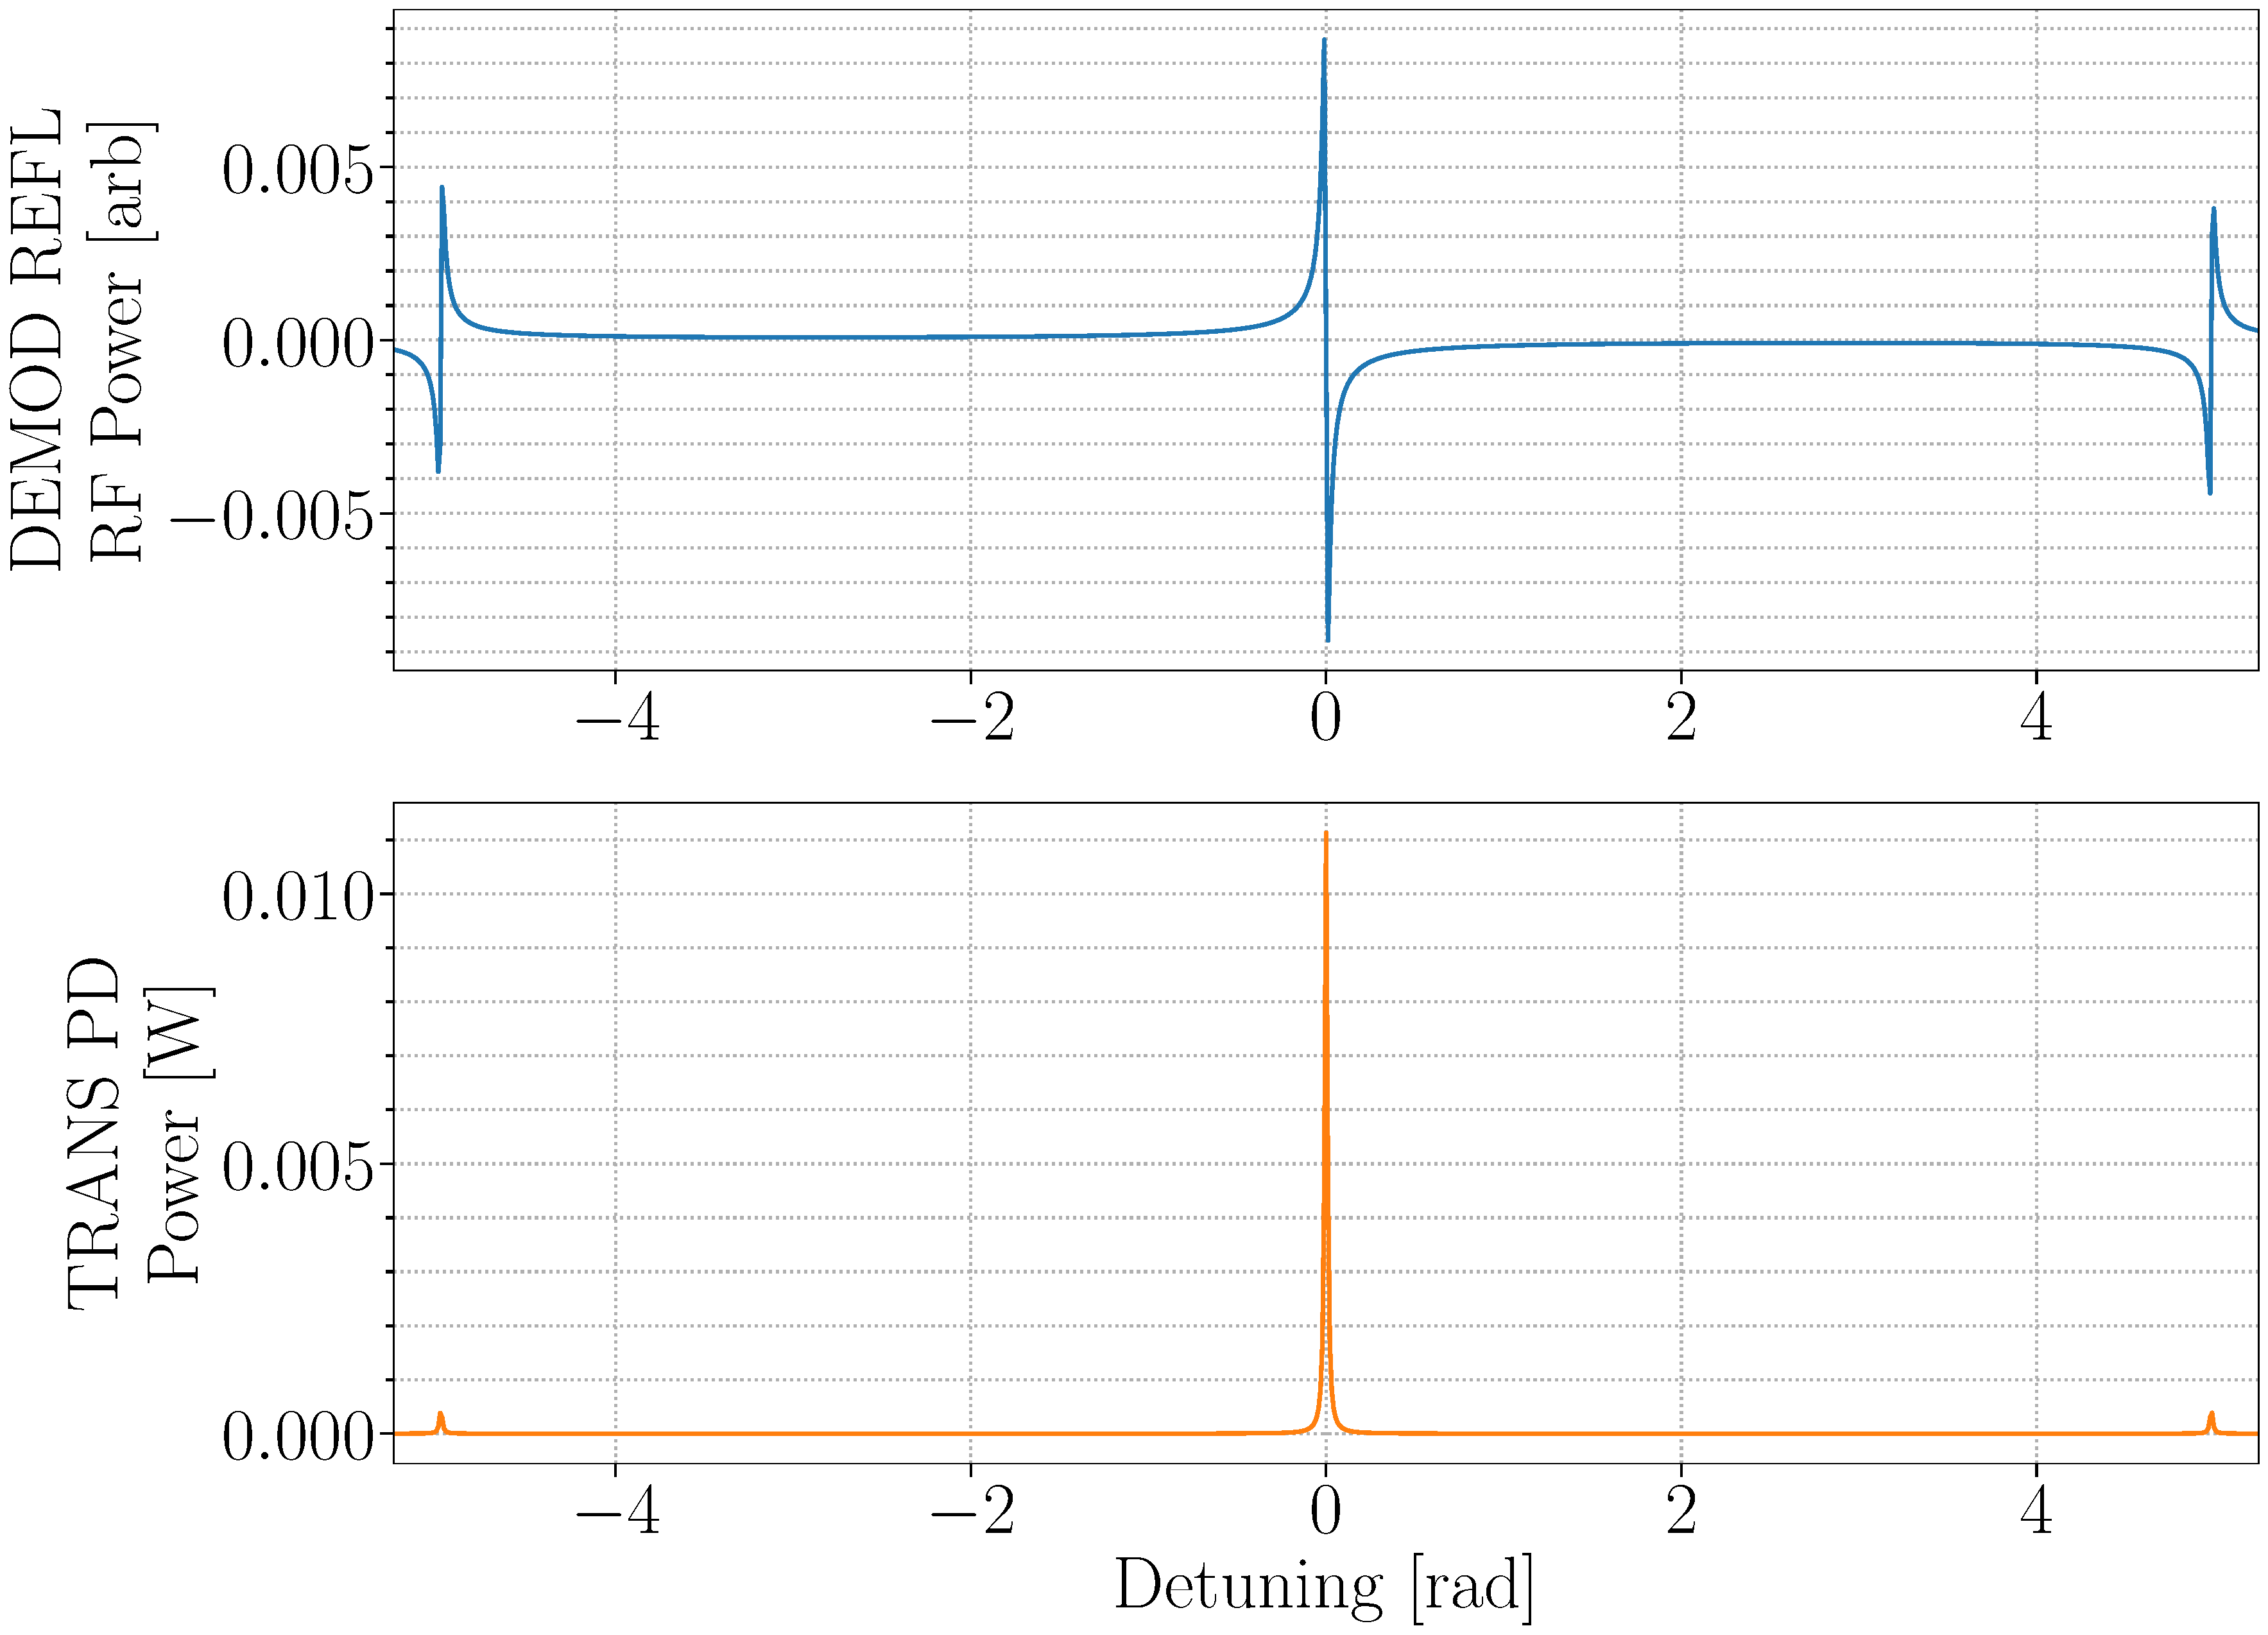
\includegraphics[width=\textwidth]{figs/ALGAAS/pdh_error.pdf}
	\caption{By imposing 25 MHz RF sidebands we have introduced a constant reflected reference field near carrier resonance which when beat with the carrier offers a linear response after demodulating the sideband power. With the introduction of high and low frequency sideband fields, their presence is also detected through the DCPDs and PDH error signal. Their separations from carrier resonance are equal in phase (length, and frequency).}
\label{fig:pdh_error}
\end{figure}

With this linearity and sensitivity at cavity resonance, implementation into PID feedback is the next task as any small detuning of the cavity can be registered as a drift from the loop's zero point and fed back to an actuator with an estimated calibration gain factor. When implemented into a low-noise design, this servo can also be used for a high sensitivity lock-in measurement; and with well characterized instrumentation, calibration of the induced differential phase of the light within the stable reference cavity into differential length (or frequency).


\subsection{Servo Parameters}
The quantity we are attempting to measure is on the order of a length change of ? m/(V/m), motivating a short cavity design as the relative differential length (phase) change scales with the sensitivity $\Delta f / f = \Delta L / L$. Considerations of the lab mirror inventory and mode matching critera lead us to two candidate plano-concave (ROC = 0.333m) HR IBS coated sample input couplers; one from CVI Melles-Griot and another from ATFilms. When paired with the plano-plano GaAs/$\mathrm{Al_{.92}Ga_{.08}As}$  mirror from the Crystalline Mirror Solutions (CMS) division of Thorlabs we create a 0.1665 m long cavity.


\begin{figure}[H]
\begin{center}
\includegraphics[width=.80\textwidth]{ALGAAS/opt_layout_b.pdf}
\end{center}
\caption{\textcolor{red}{Final figure still pending} Detailed optical schema of the experiment. Components highlighted in magenta indicate laser back-reflection protection and output power control. All optics highlighted in PURPLE indicate their function as alignment and mode matching for locking to a triangular ALIGO PMC \textbf{Multiple citations (DCC doc / Fabian's experiment / Erik's experiment)}. Optics highlighted in YELLOW indicate function for alignment and mode matching to the experimental cavity utilizing the HR $\gaas$/$\algaas$ coated mirror sample. Beam profiling to the sample cavity is indicated. For the sake of the numerous mounting strategies tried, the longitudinal pockels cell mirror mount is kept general with the pictured mirror between two disk capacitors}
\label{fig:detailed_optical_layout}
\end{figure}
%%FIGURE: Servo diagram
%%CAPTION: A simplified diagram of the servo used. The highlighted regions of the schematic are intended to provide a modular view; highlighting the components required for the PDH servo to operate.}
The implemented servo design uses a light source from a Mephisto 2000 NE Nd:YAG (1064nm) laser with a 25 MHz phase modulation from a New Focus Model 4003 IR resonant phase modulator. As indicated in the figure above, the electronics chain can be decomposed into various filter components: $S(f)$, $A(f)$, and $A_\mathrm{thermal}(f)$

\subsubsection{Sensing S(f)}
The sensing filter electronics are composed of a single element photodiode (from?) with a QE of ? and the response found in appendix ?. The signal is then mixed with a 25 MHz oscillator phased 180 degrees ? m of cable so the measured beat signal while sweeping through resonance generates the \hyperref[fig:pdh_error]{PDH error signal profile}.
\begin{itemize}
\item 25 MHz RFPD
\begin{itemize}
\item Transimpedance measurement (necessary? or should I just use the mixer out PDH to summarize PD/mixer response)
\end{itemize}
\item Frequency Stabilization servo (modified MIT FSS (DCCD980536)) (LTspice model in appendix)
\end{itemize}


\subsubsection{Actuation A(f)}
\begin{itemize}
\item Mephisto 2220 PZT response (capacitance estimated from HVA drive measurement with and without connection to PZT)
\item Channel 3 of SVR 350-3 BIP High Voltage Amplifier from Piezomechanik GmbH with Pomona box (elog 412)
%%FIGURE: Frequency response of A(f)}

\end{itemize}

\subsubsection{Low frequency servo (Thermal loop)}
\begin{itemize}
\item Passed signal from FSS $\rightarrow$ integrators $\rightarrow$ Laser thermal actuator input
\end{itemize}

\subsubsection{OLG(f)}
Isn't quite $\mathrm{A}(f)*\mathrm{S}(f)$ as stated. Doesn't entirely account for the optical plant.
How the measurement is taken (important to take between installations to account for the changes in the optical plant) (elog 831)

\begin{figure}[H]
\begin{center}
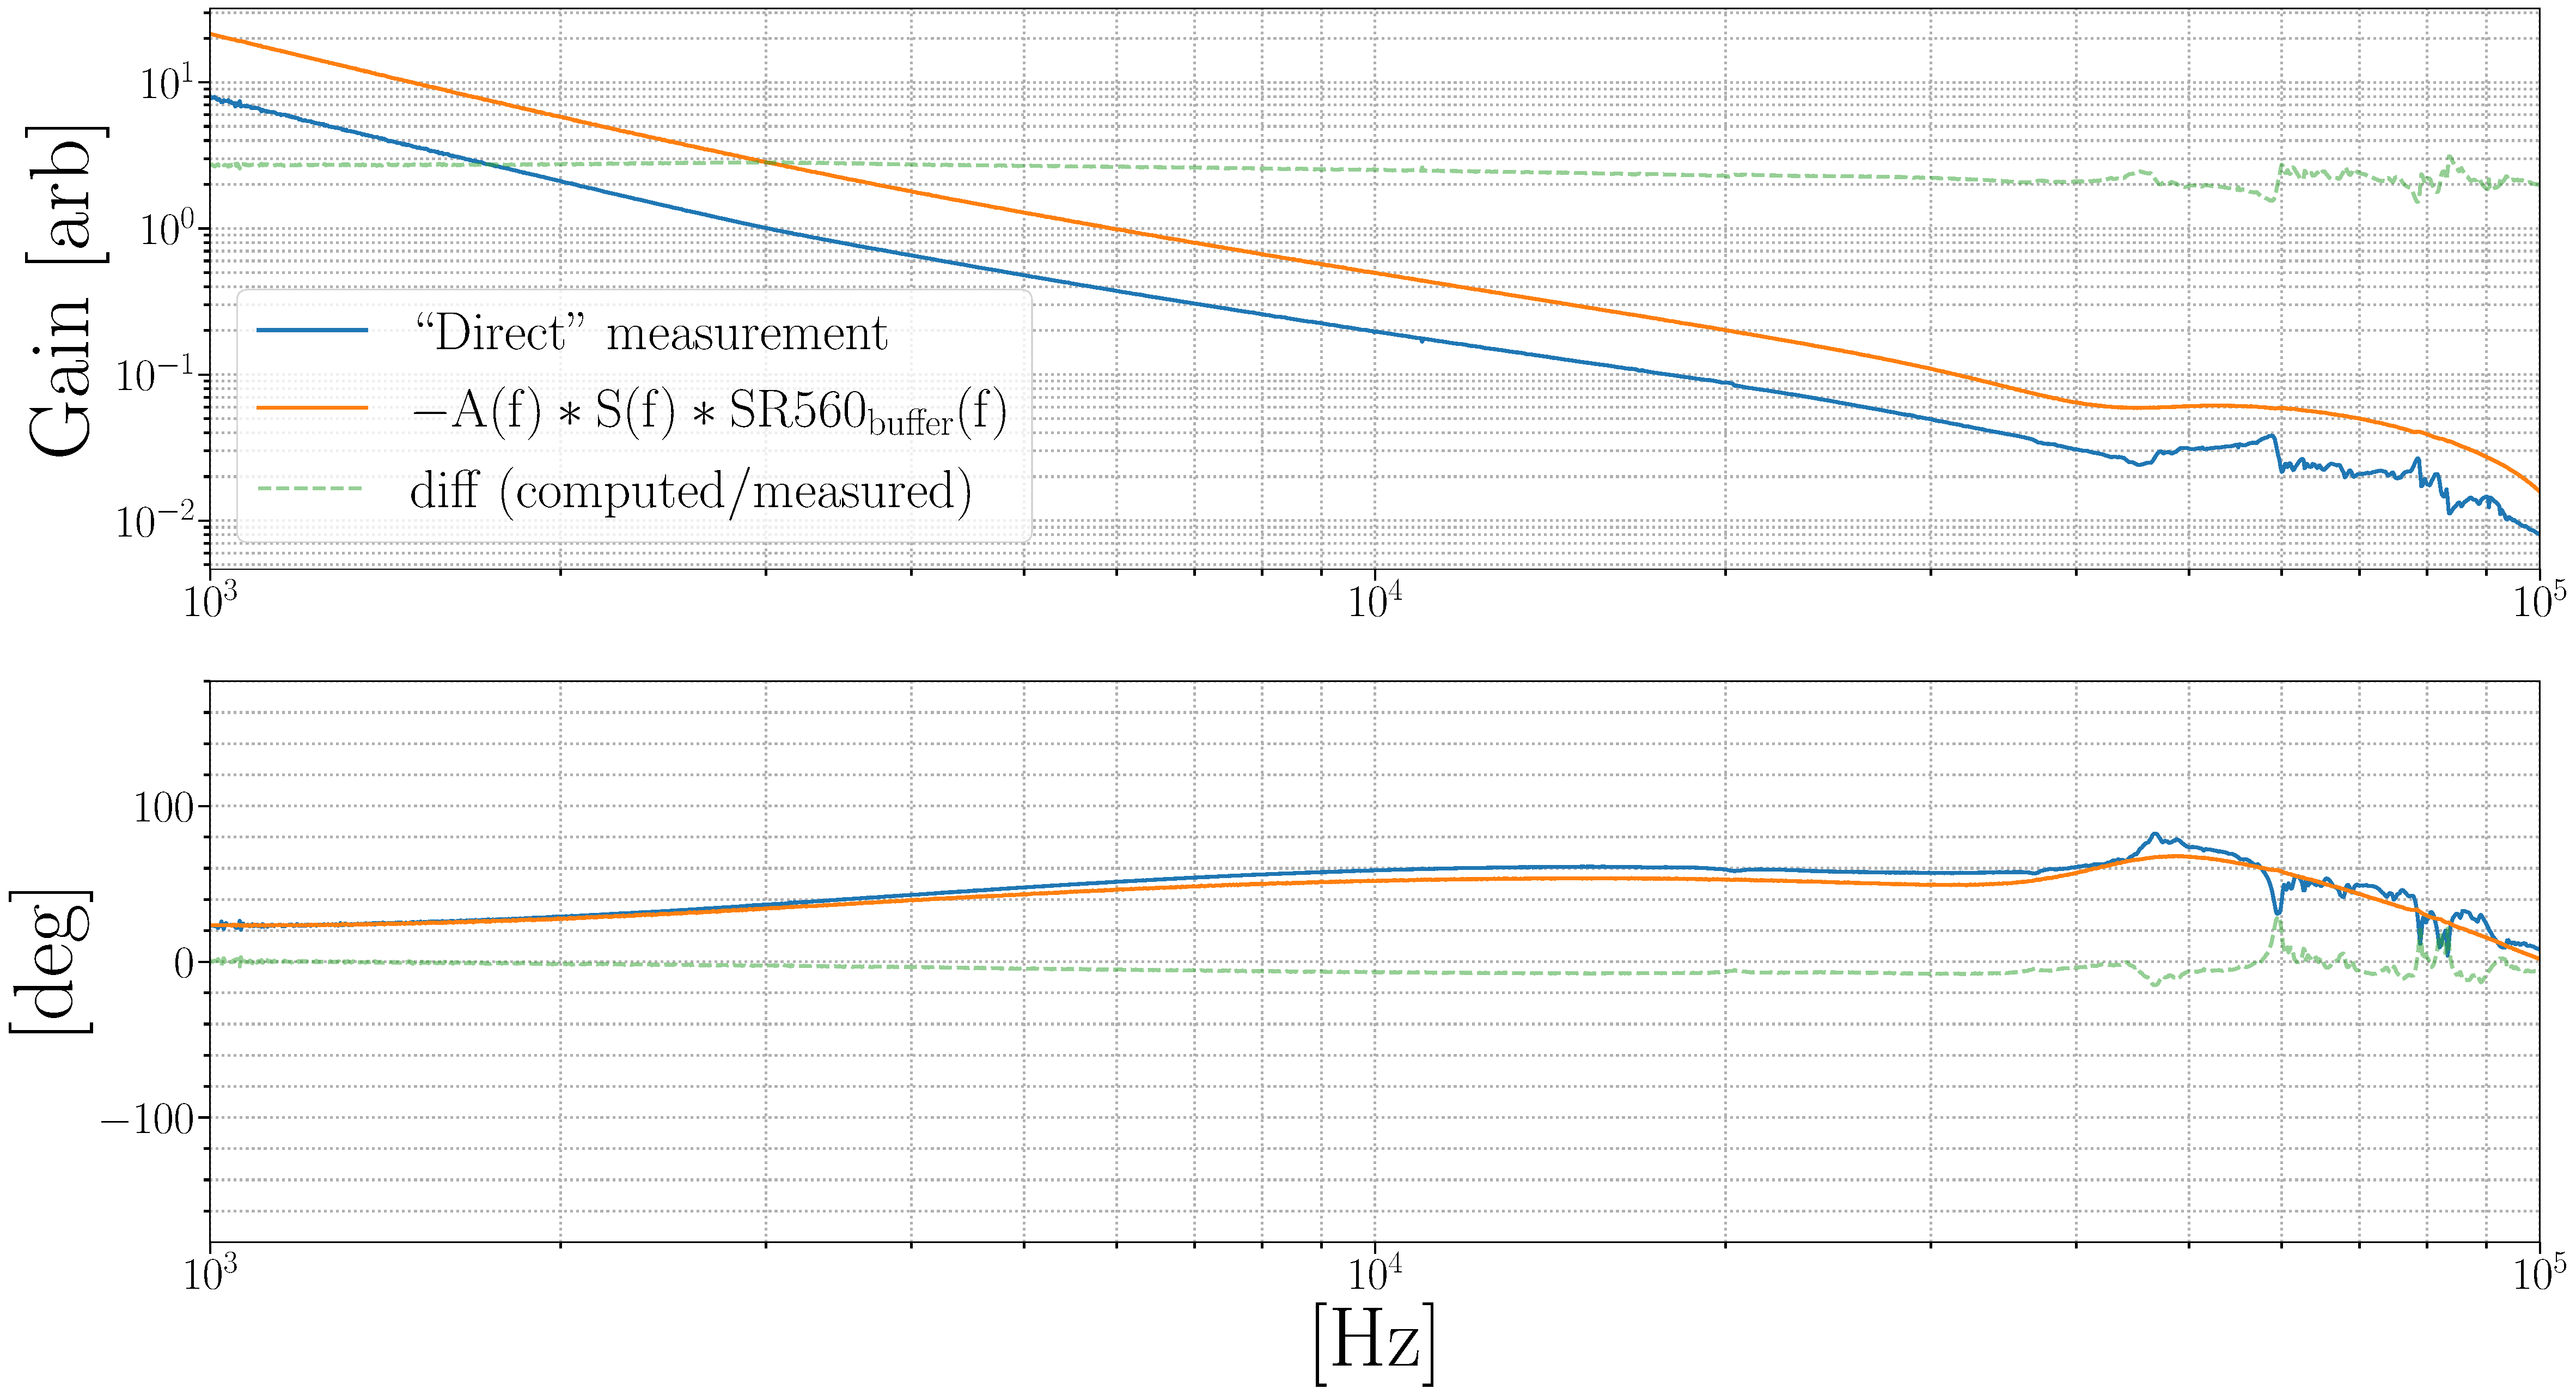
\includegraphics[width=\textwidth]{ALGAAS/olg_compare.pdf}
\end{center}
\caption{Comparison of the open loop gain measurement against the multiplied servo electronics measurements. The maximum gain difference is about a factor of 2.8 which is low passed to a difference of 2.0.}
\label{fig:OLG_compare}
\end{figure}


\subsection{Longitudinal Pockels Cell mirror mount assembly}
Maximizing a controlled and well defined electric field ($|E_z|$) within the coating while requiring a through beam to and through the HR coating lead us to a design very similar to that of a longitudinal pockels cell \cite{}. The most common assembly in for this study is comprised of two electrodes with a 3mm central aperture which is chosen to be at least 5 times larger than the beam size at the plate locations; to avoid significant beam clipping while maximizing field strength at the coating region of interest. There is also a required separation of at least 1/4" accounting for the thickness of the optical sample. Considering these constraints, modelling the system and computing the estimated field strength screened by the coating is the next step to the construction of the assembly.

\begin{figure}[H]
\begin{center}
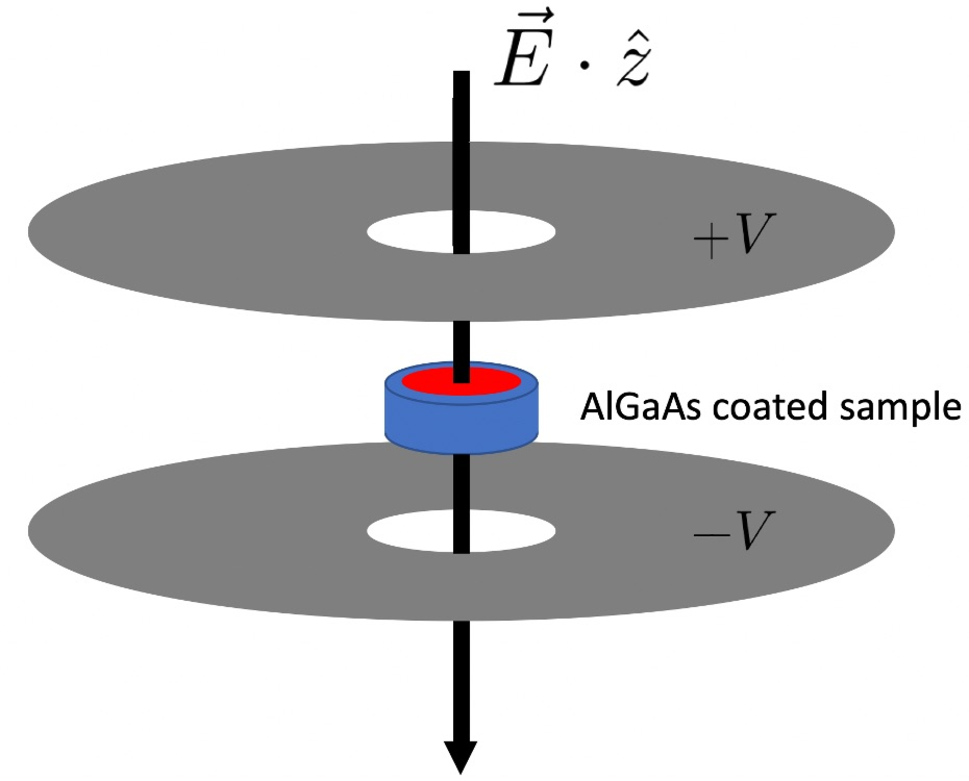
\includegraphics[width=.7\textwidth]{ALGAAS/assemblies/disk_electrode_concept.pdf}
\end{center}
\caption{Concept image of the longitudinal Pockels cell assembly}
\label{fig:pock_cell_assembly_concept}
\end{figure}

\subsubsection{Modelling}

To find the Electric field screened by the coating we begin with Gauss' Law:

\begin{equation}
\nabla \cdot D = \rho_\mathrm{free}
\end{equation}
For our problem we assume no free charge, but the fused silica substrate with the AlGaAs coating presents dielectric material between the plates. Our initial boundary conditions are also expressed in terms of plate potentials so it is natural to first solve for the potential ($V$) for every point within our system. We can exploit the cylindrical symmetry with the optic and plate geometry in the $r$ coordinate so we shall express the Laplacian accordingly:
\begin{equation}
\bigg[\frac{1}{r}\frac{\partial}{\partial r} \bigg( r \frac{\partial}{\partial r}\bigg) + \frac{\partial^2}{\partial z^2}\bigg](\varepsilon V) = 0
\end{equation}
Where $\varepsilon$ is the dielectric

\begin{figure}[H]
  \centering
  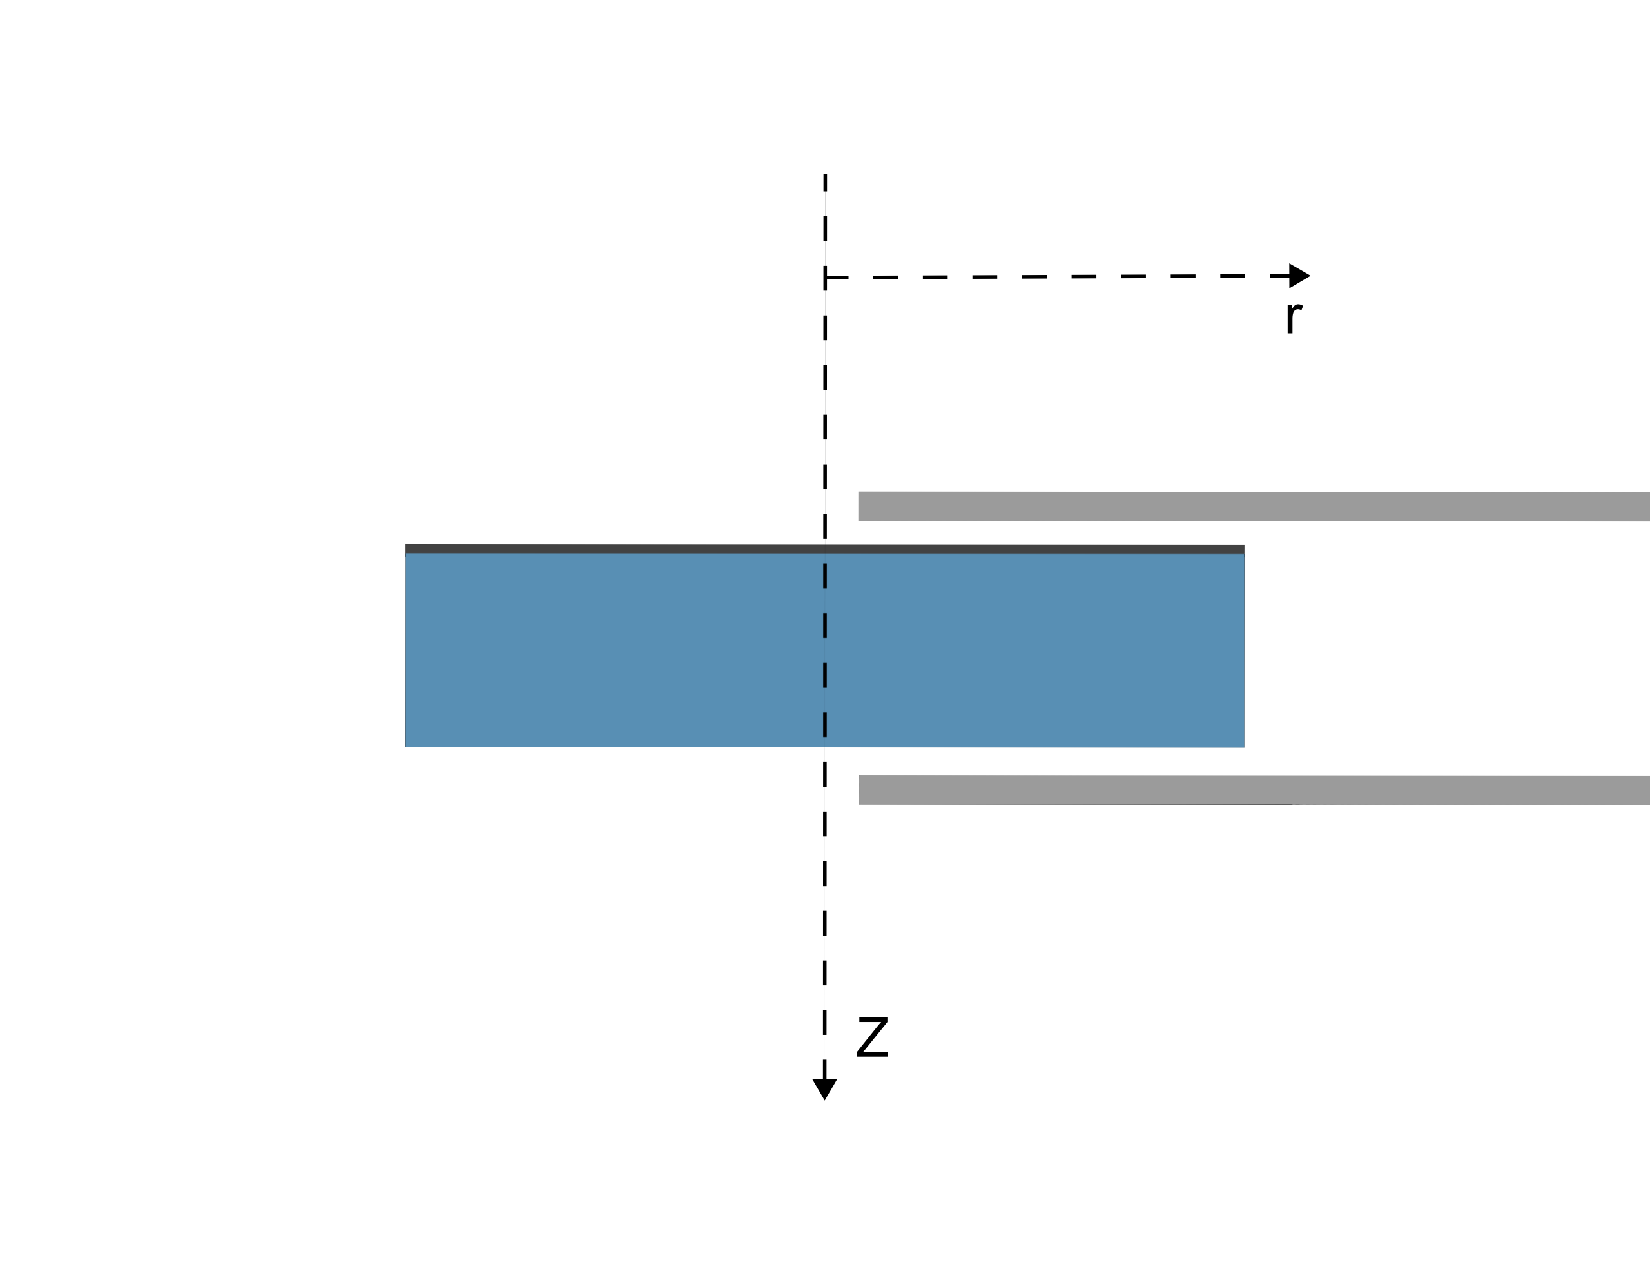
\includegraphics[width=.65\textwidth]{figs/ALGAAS/laplace_coord_test.pdf}
  \caption{\textcolor{red}{PENDING}}
  %%Use relevant cross sectional figure to establish coordinates for $\gaas$/$\algaas$, as well as the fused silica substrate so the computation is transparent.} Cross sectional diagram indicating relevant axes and boundary conditions utilized in the numerical computation
  \label{fig:laplace_coords}
\end{figure}

%%Numerical recipe in appendix

\begin{itemize}
\item Potential map computation in cylindrical
\item Computing $E_z$ from potential map
\begin{itemize}
\item inside coating
\item outside coating
\end{itemize}
\end{itemize}


\begin{figure}[H]
  \includegraphics[width=\textwidth]{ALGAAS/assembly1_sim.pdf}
  \caption{Poisson calculator output potential map ($V(z,r)$ in cylindrical coordinates)}
  \label{fig:poisson_calc_output}
\end{figure}

\subsubsection{Voltage drive electronics}

\begin{figure}[H]
    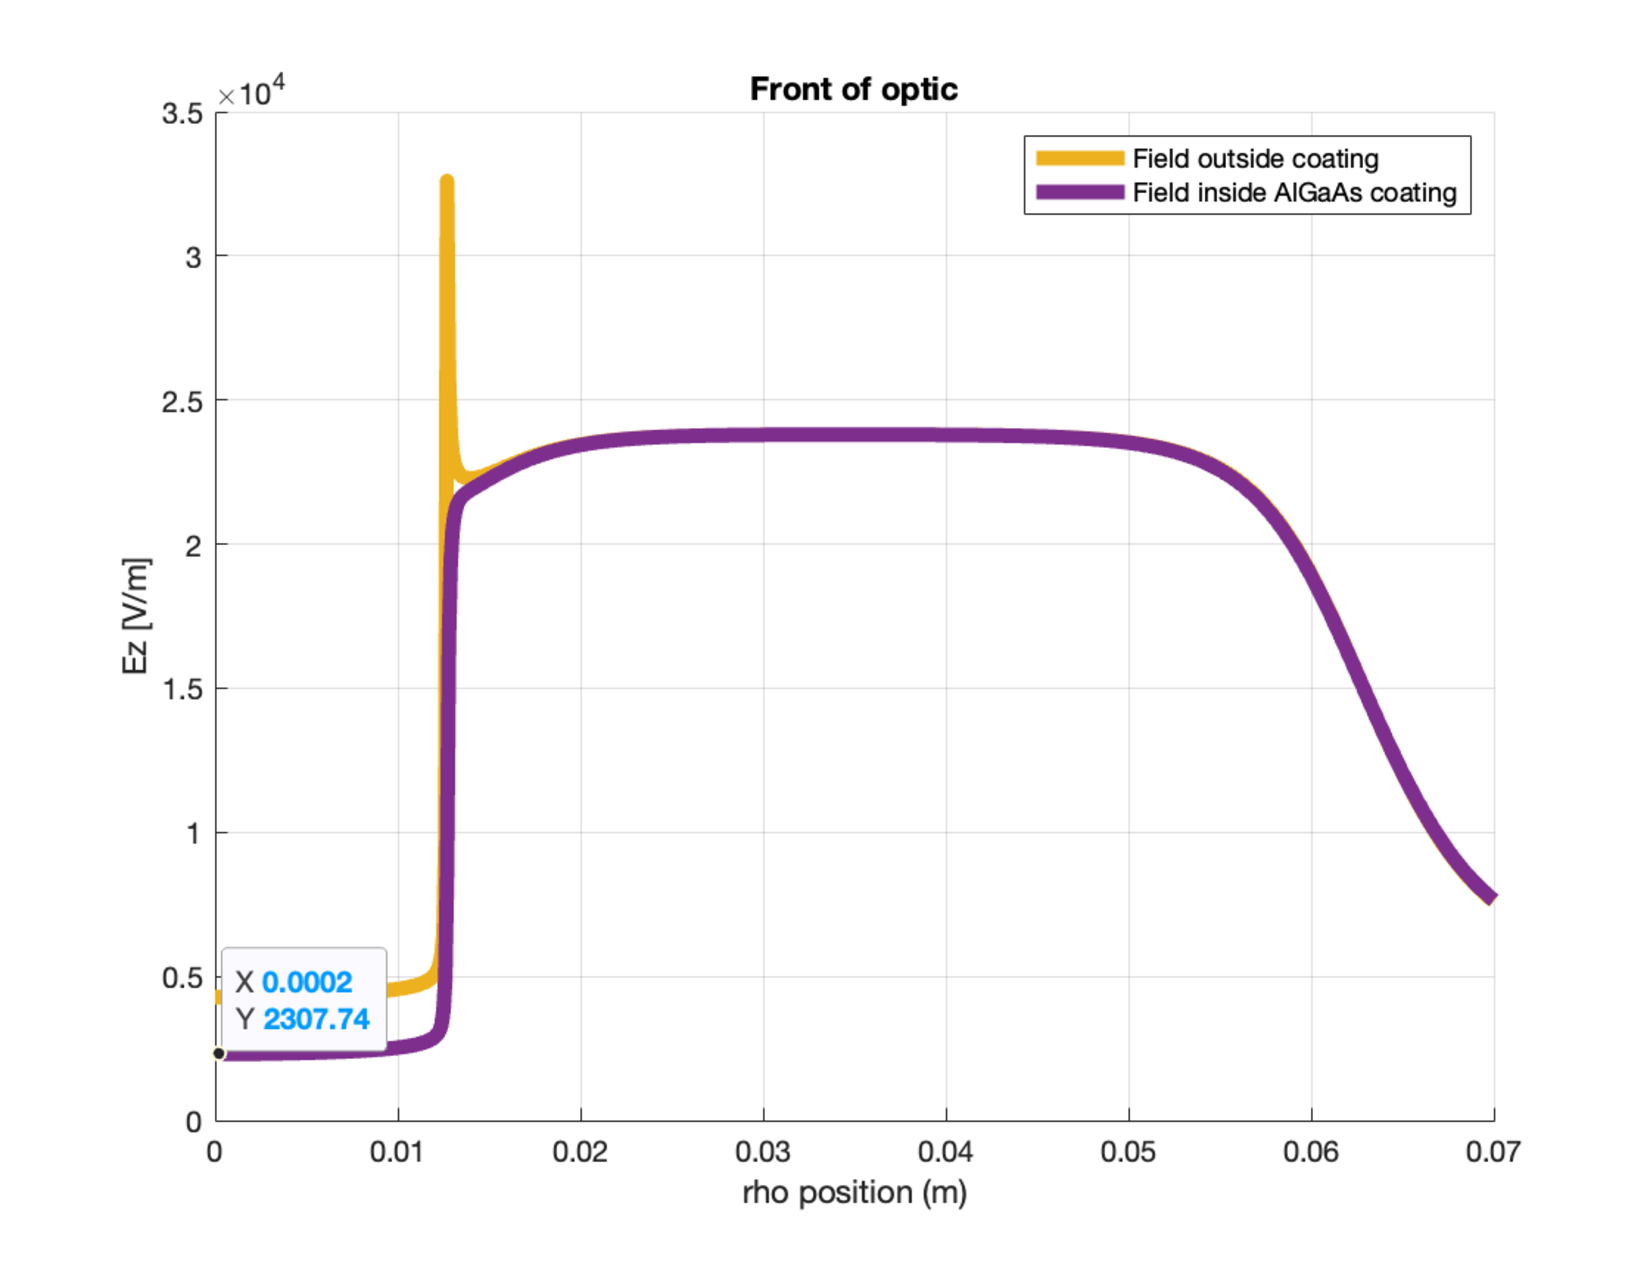
\includegraphics[width=\textwidth]{ALGAAS/13-Sep-2021_e_field_inside_outside_normal.pdf}
    \caption{The availablility of required voltage amplifiers during the course of this study was limited and lead to the use of multiple high voltage amplifiers with all transfer functions listed.}
\label{fig:Ez}
\end{figure}


\begin{figure}[H]
    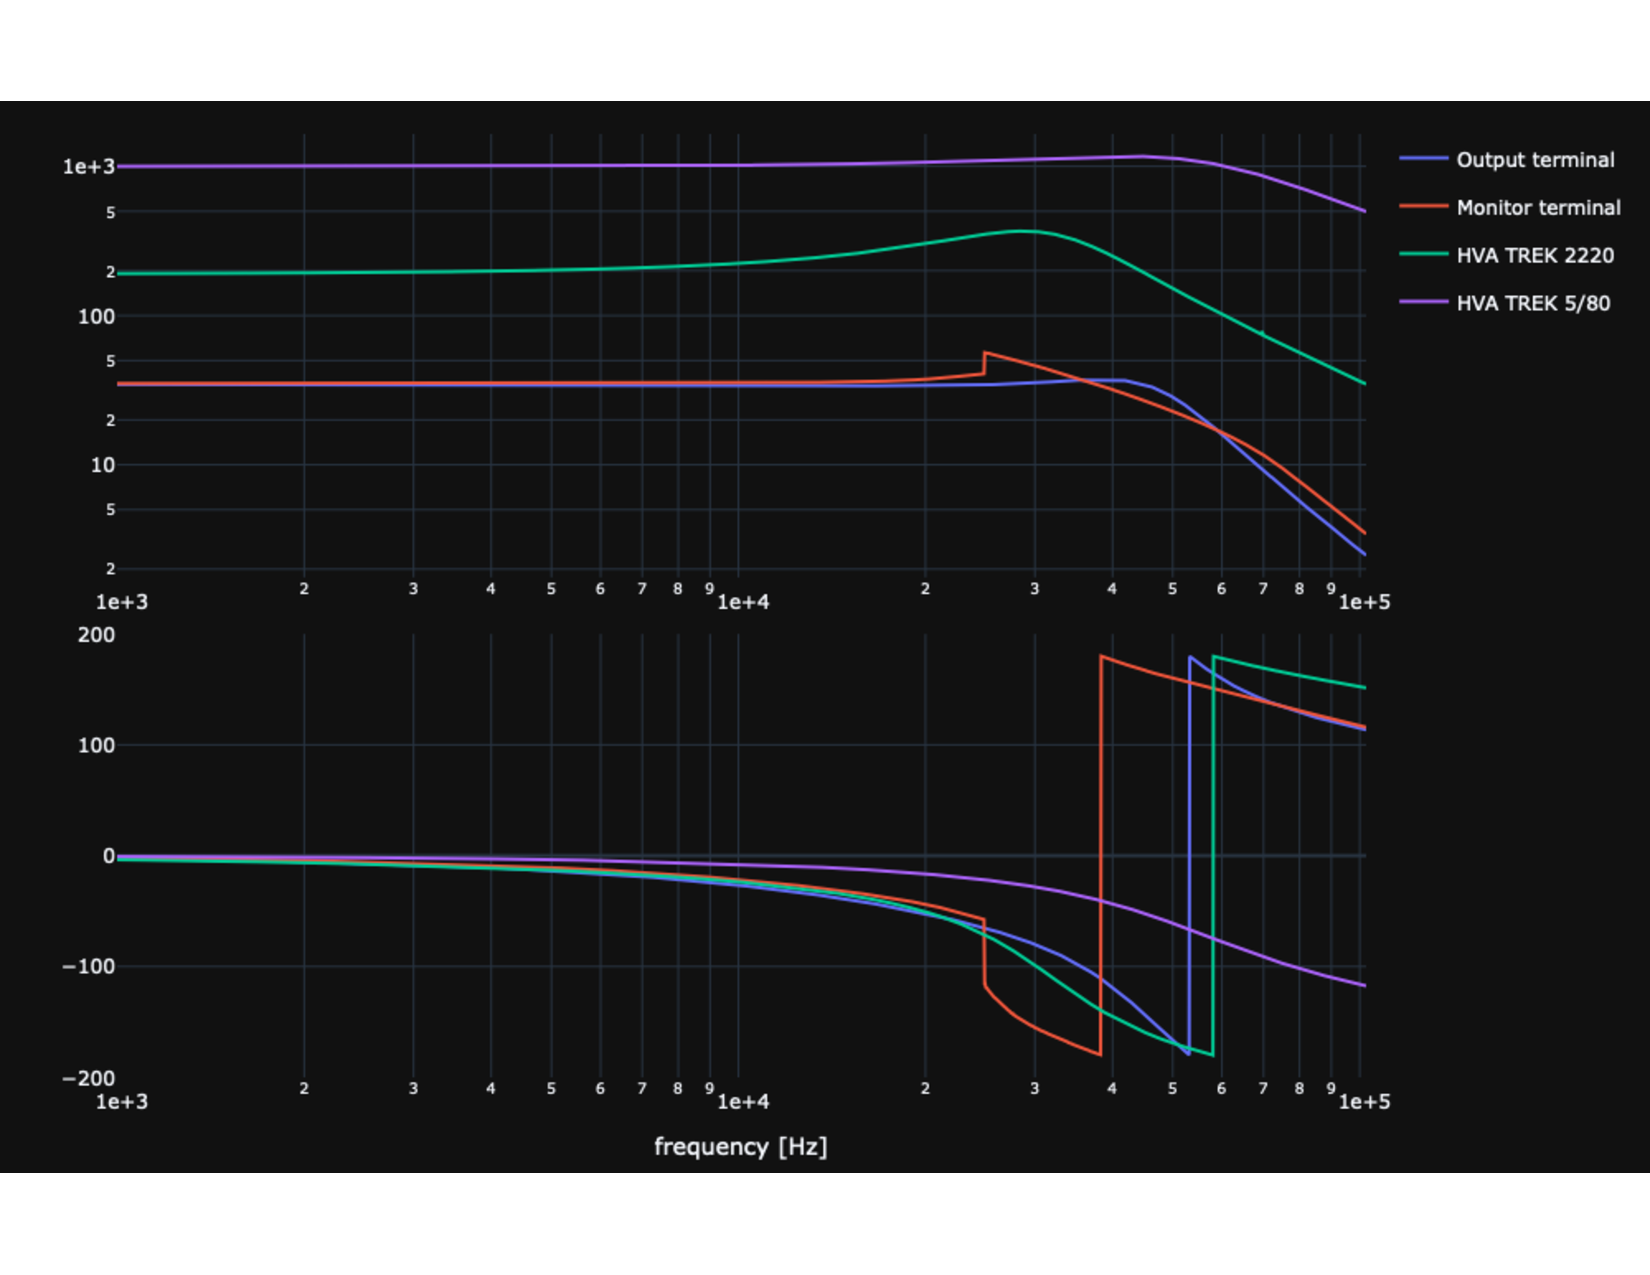
\includegraphics[width=\textwidth]{ALGAAS/tfs/hva_compare.pdf}
    \caption{Different high voltage amplifier transfer functions used for the study}
    \label{fig:hva_compare}
\end{figure}

\section{Results}
Significant barriers were encountered in the form of cavity differential length noise especially when mounting the optics in accessible non-conductive materials. Most commercial optical mounts are constructed with conducting materials which proved to be a barrier when attempting to find a mounting solution while reducing non-normal field gradients within the coating volume of interest within the sample. For this reason, efforts were focused on developing a suitable mounting solution that would provide adequate isolation from any uncontrolled field magnitudes while driving a field normally incident on the surface with enough strength and uniformity across the beam area to extract a measurement of the differential length change from the Pockels effect. The mounts studied span different geometries and different material properties. The varying geometrical assembly differences created distinguishable mount solutions, and it is how this section will be divided. For reassurance, we compare displacement spectra against that of a nearly identical cavity with a flat non-crystalline mirror coating to perform a null measurement reference; ruling out the Pockels effect and providing information for noise investigations.

\subsection{Measurement Calibration}
The error signal spectra probed at the FSS:

\begin{equation}
\mathrm{VFSSOUT}_\mathrm{rms}/\sqrt{Hz} \rightarrow m_\mathrm{rms}/\sqrt{\mathrm{Hz}}
\end{equation}

With the known frequency response of the servo electronics, we \hyperref[sec:calibration]{calibrate} the measurement into differential length:
\begin{equation}
	\Delta \mathrm{L} = \mathrm{source}*\alpha(f) \mathrm{A}(f)*\frac{1+\mathrm{OLG}(f)}{\mathrm{OLG}(f)}*\frac{\mathrm{L_{cav}}}{f_\mathrm{laser}} \quad \big[ m_\mathrm{pk} / \sqrt{Hz} \big]
\end{equation}

\subsection{Mounting Strategies}
The following section details measurements performed with various longitudinal pockel cell mounts. Further details (assembly parameters, blueprints, and visual aids) can be found in the appendix.

\subsubsection{Assembly 1}

\begin{figure}[!ht]
    \begin{subcaptiongroup}
	    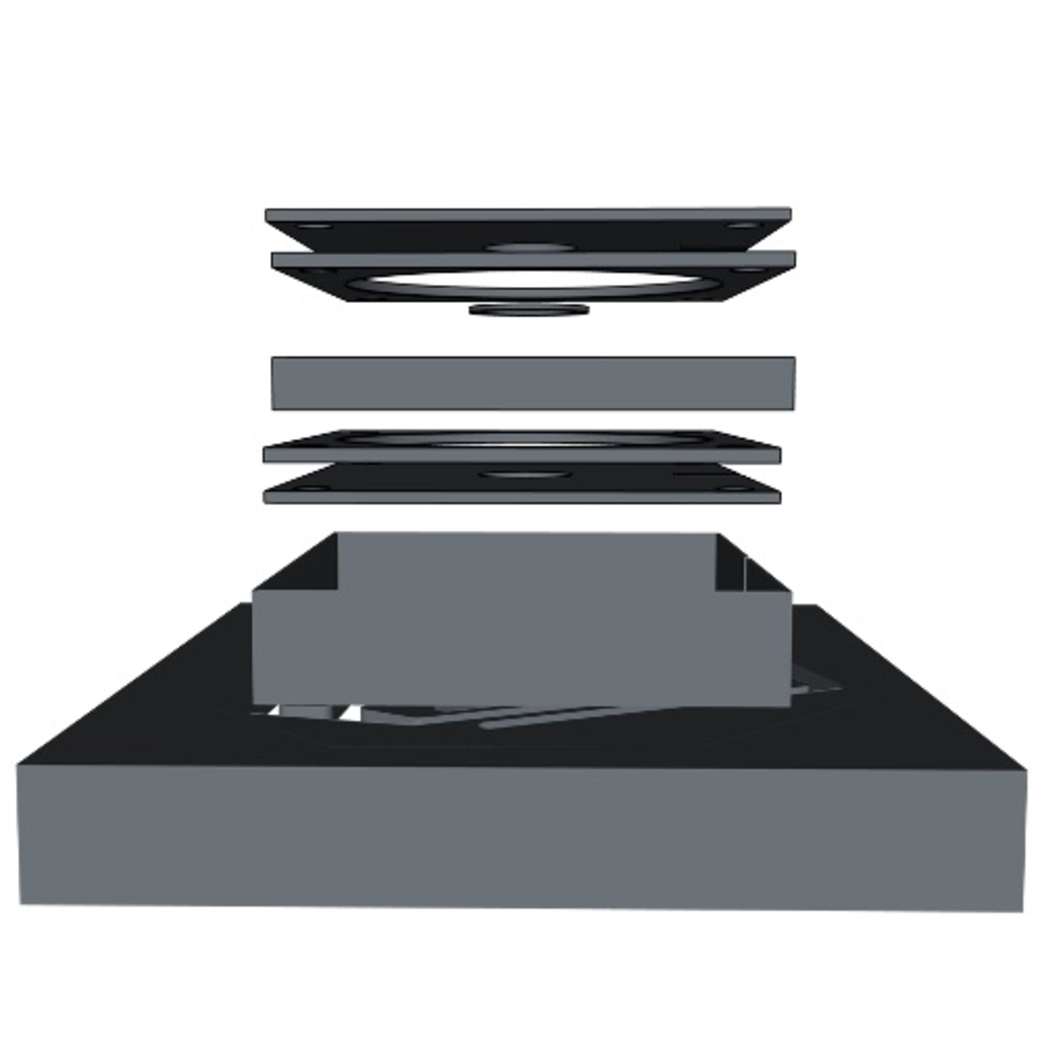
\includegraphics[width=.5\textwidth]{figs/ALGAAS/assemblies/assembly1/assembly1_dissassembled.pdf}
	    \phantomcaption\label{A1_disassembled}
	    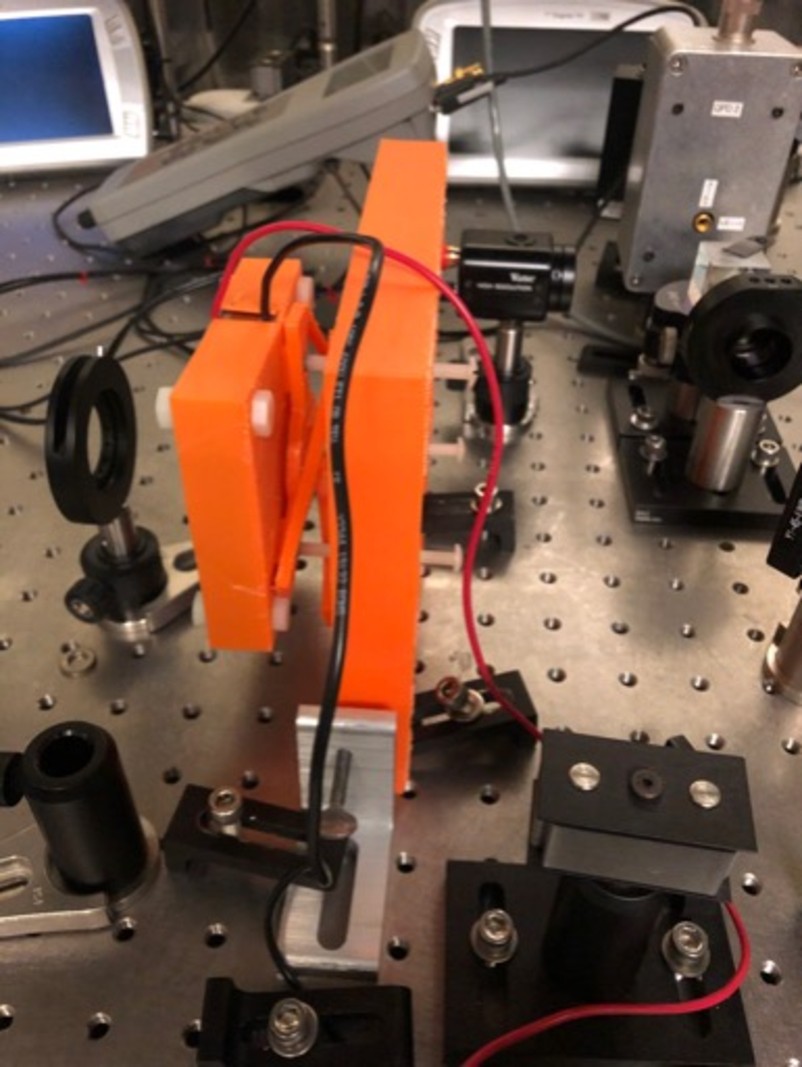
\includegraphics[width=.5\textwidth]{figs/ALGAAS/assemblies/assembly1/assembly1_flaw.pdf}
	    \phantomcaption\label{A1_flaw}
    \end{subcaptiongroup}
    \caption{Assembly 1 was constructed to meet two criteria: the same solution of housing the sample and electrodes as Assembly 0, but also offer pitch / yaw control via an ortho-planar spring design (Brigham Young University).}
    \label{fig:A1pt0}
\end{figure}
\FloatBarrier


The construction revealed flaws; made most obvious when comparing to displacement noise of traditional optical mounts. Pitch and yaw control via the ortho-planar spring were prioritized to avoid metal springs and further mount pieces. The solution became unjustifiable when observing the the displacement noise coupling from the mount.

%%Re-run this calibration with adequate voltage normalization for a response unit [$m_\mathrm{pk} / [V / m]$]

\begin{figure}[H]
\centering
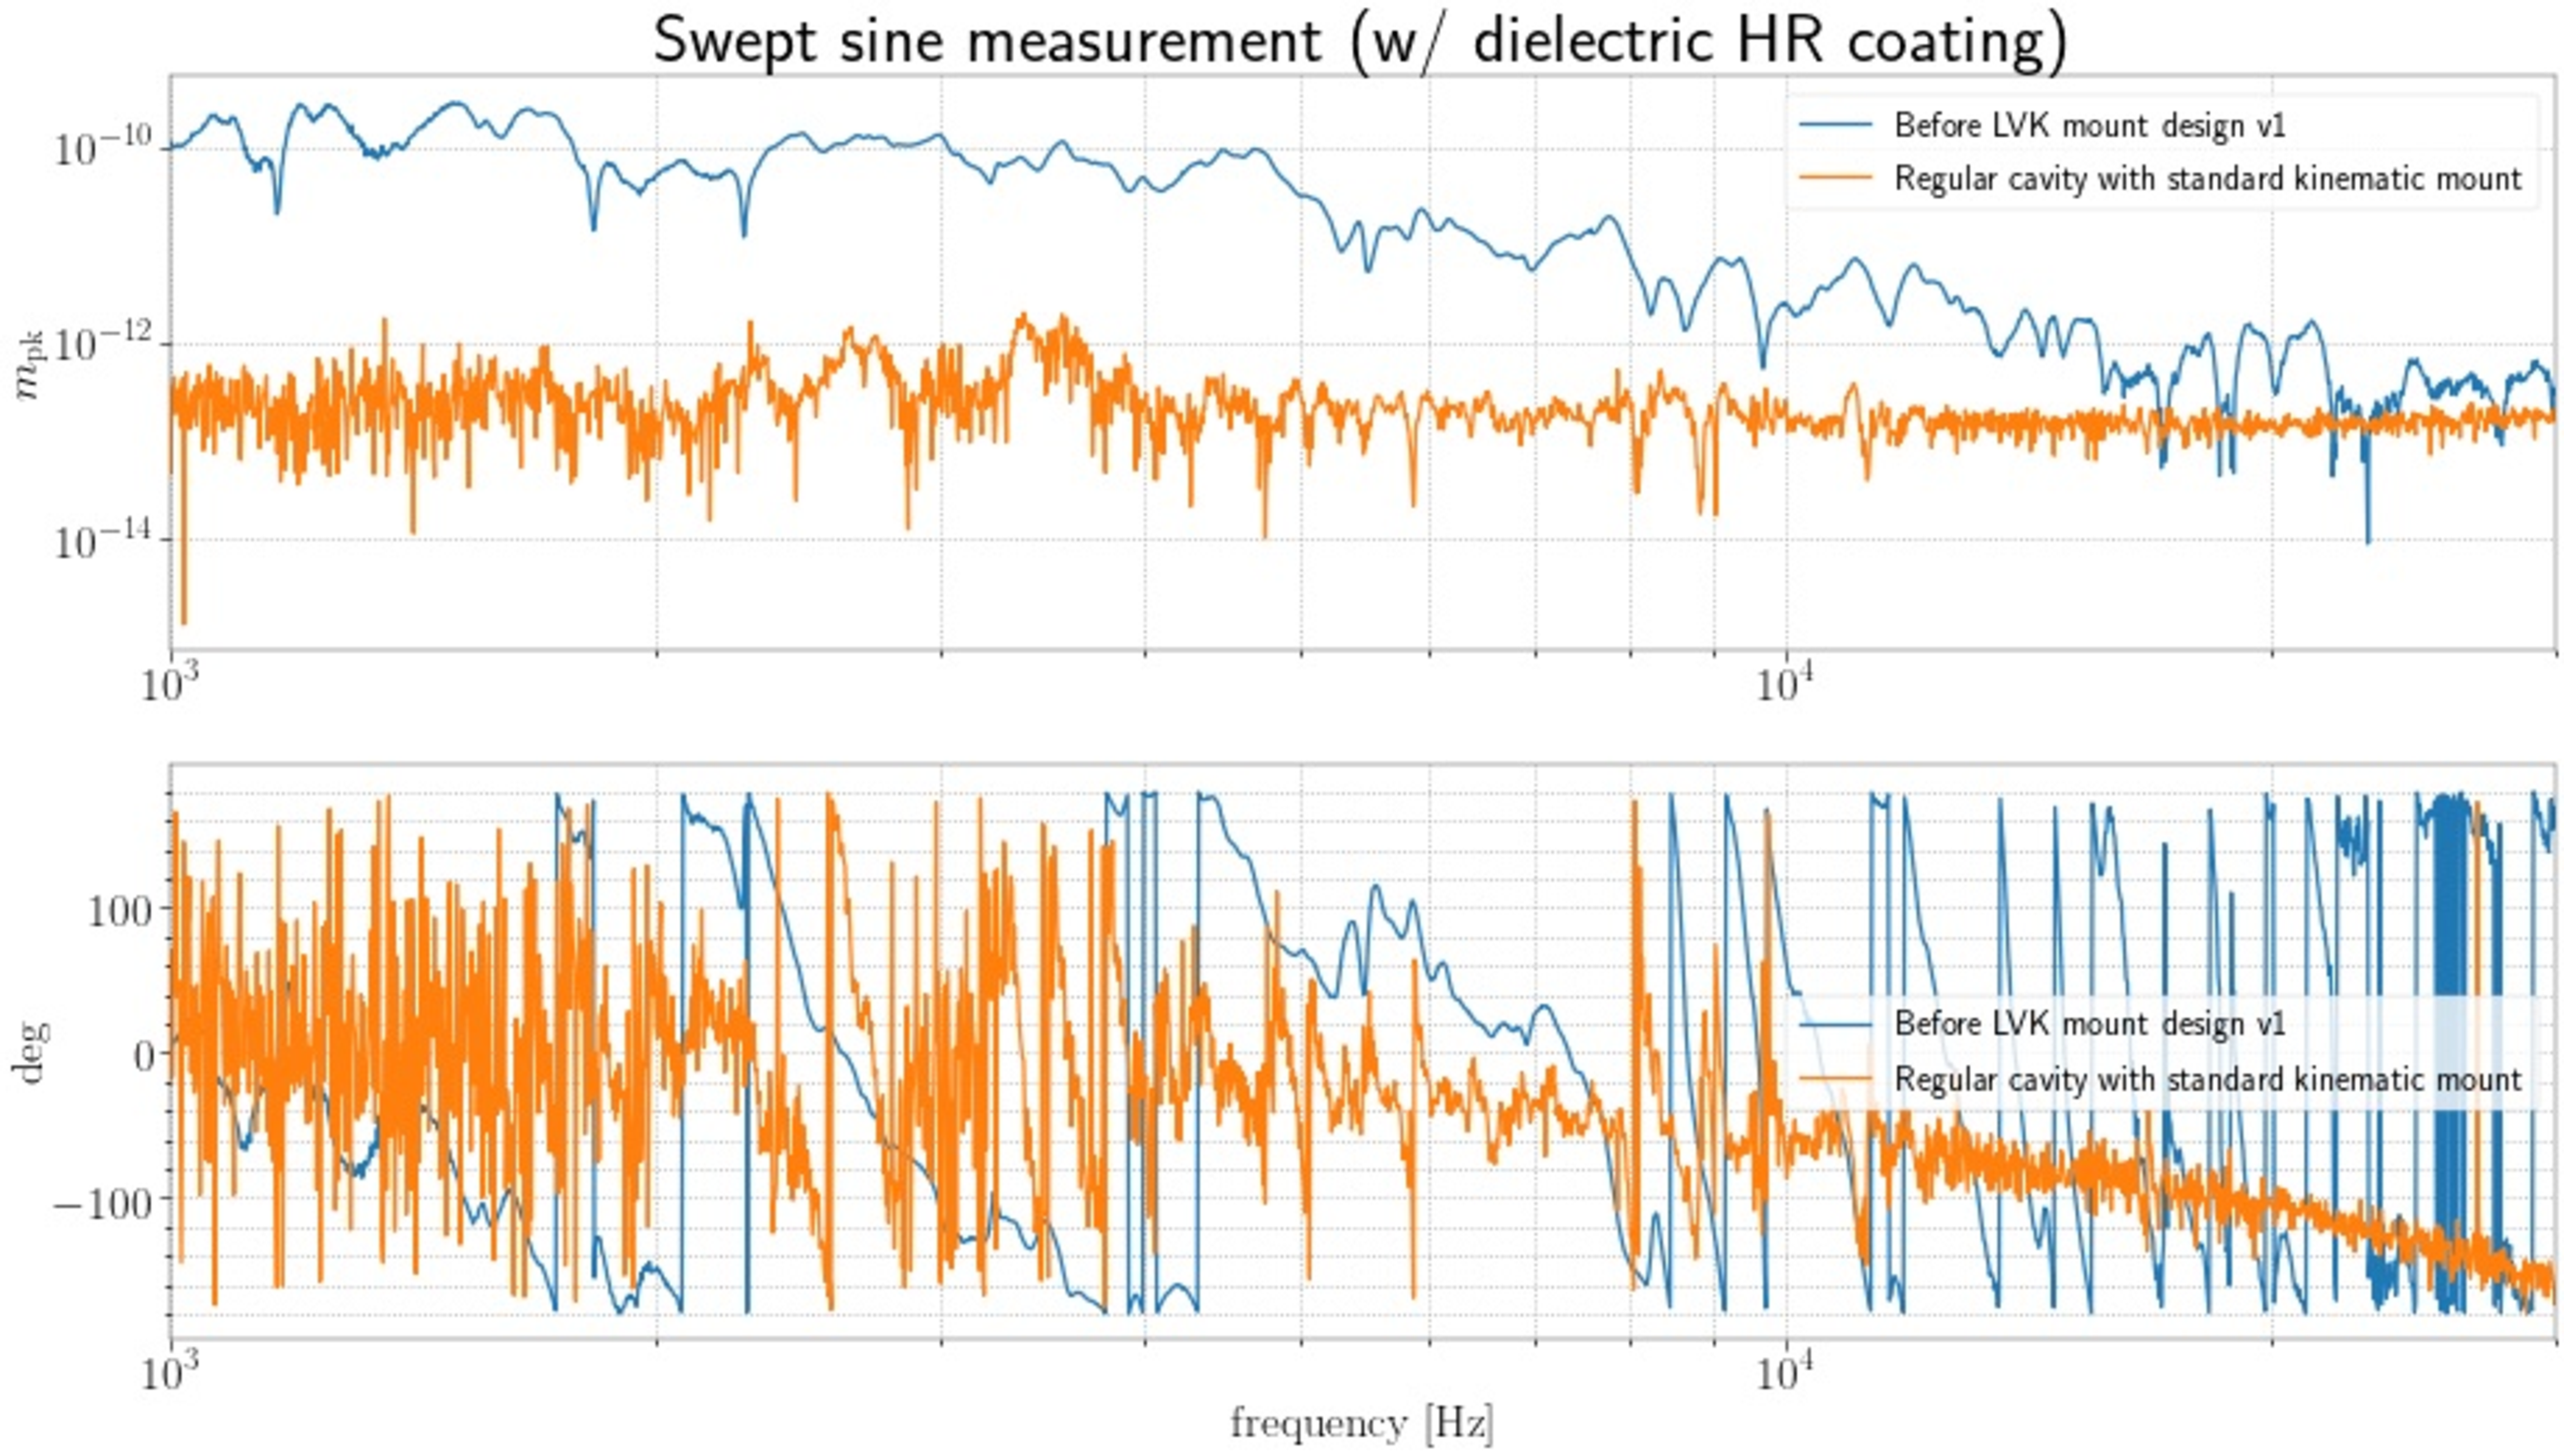
\includegraphics[width=\textwidth]{figs/ALGAAS/assemblies/assembly1/assembly1_2_compare_standmount.pdf}
\caption{Measured displacement spectra for Assembly 1.2 of the longitudinal pockels cell mount compared to the standard kinematic mount. Both measurements were recorded with the the CVI Melles-Griot (amorphous) mirror coating sample installed in the assembly.}
%%Units and legend labels need increase in font size. Remove Swept sine measurement title.
\label{fig:assembly2_compare_kinematic_mount}
\end{figure}


Attempts at improving the pitch dithering were tried with side set screws but mostly caused significant misalignment (less power in fundamental mode, locking issues, etc.). This lead to the final alternative for this assembly type; with the same PLA stack indicated in ~\hyperref[fig:A1pt0]{Assembly 1}.

\begin{figure}[!ht]
	\begin{subcaptiongroup}
		\includegraphics[width=.5\textwidth]{figs/ALGAAS/assemblies/assembly1/assembly1_mod_front.pdf}
		\phantomcaption\label{A1_front}
		\includegraphics[width=.5\textwidth]{figs/ALGAAS/assemblies/assembly1/assembly1_mod_side.pdf}
		\phantomcaption\label{A1_side}
	\end{subcaptiongroup}
    \caption{A modification implemented  with the intention of reducing pitch dithering while still having control of DC YAW}
    \label{fig:A1pt0mod}
\end{figure}

\begin{figure}[H]
    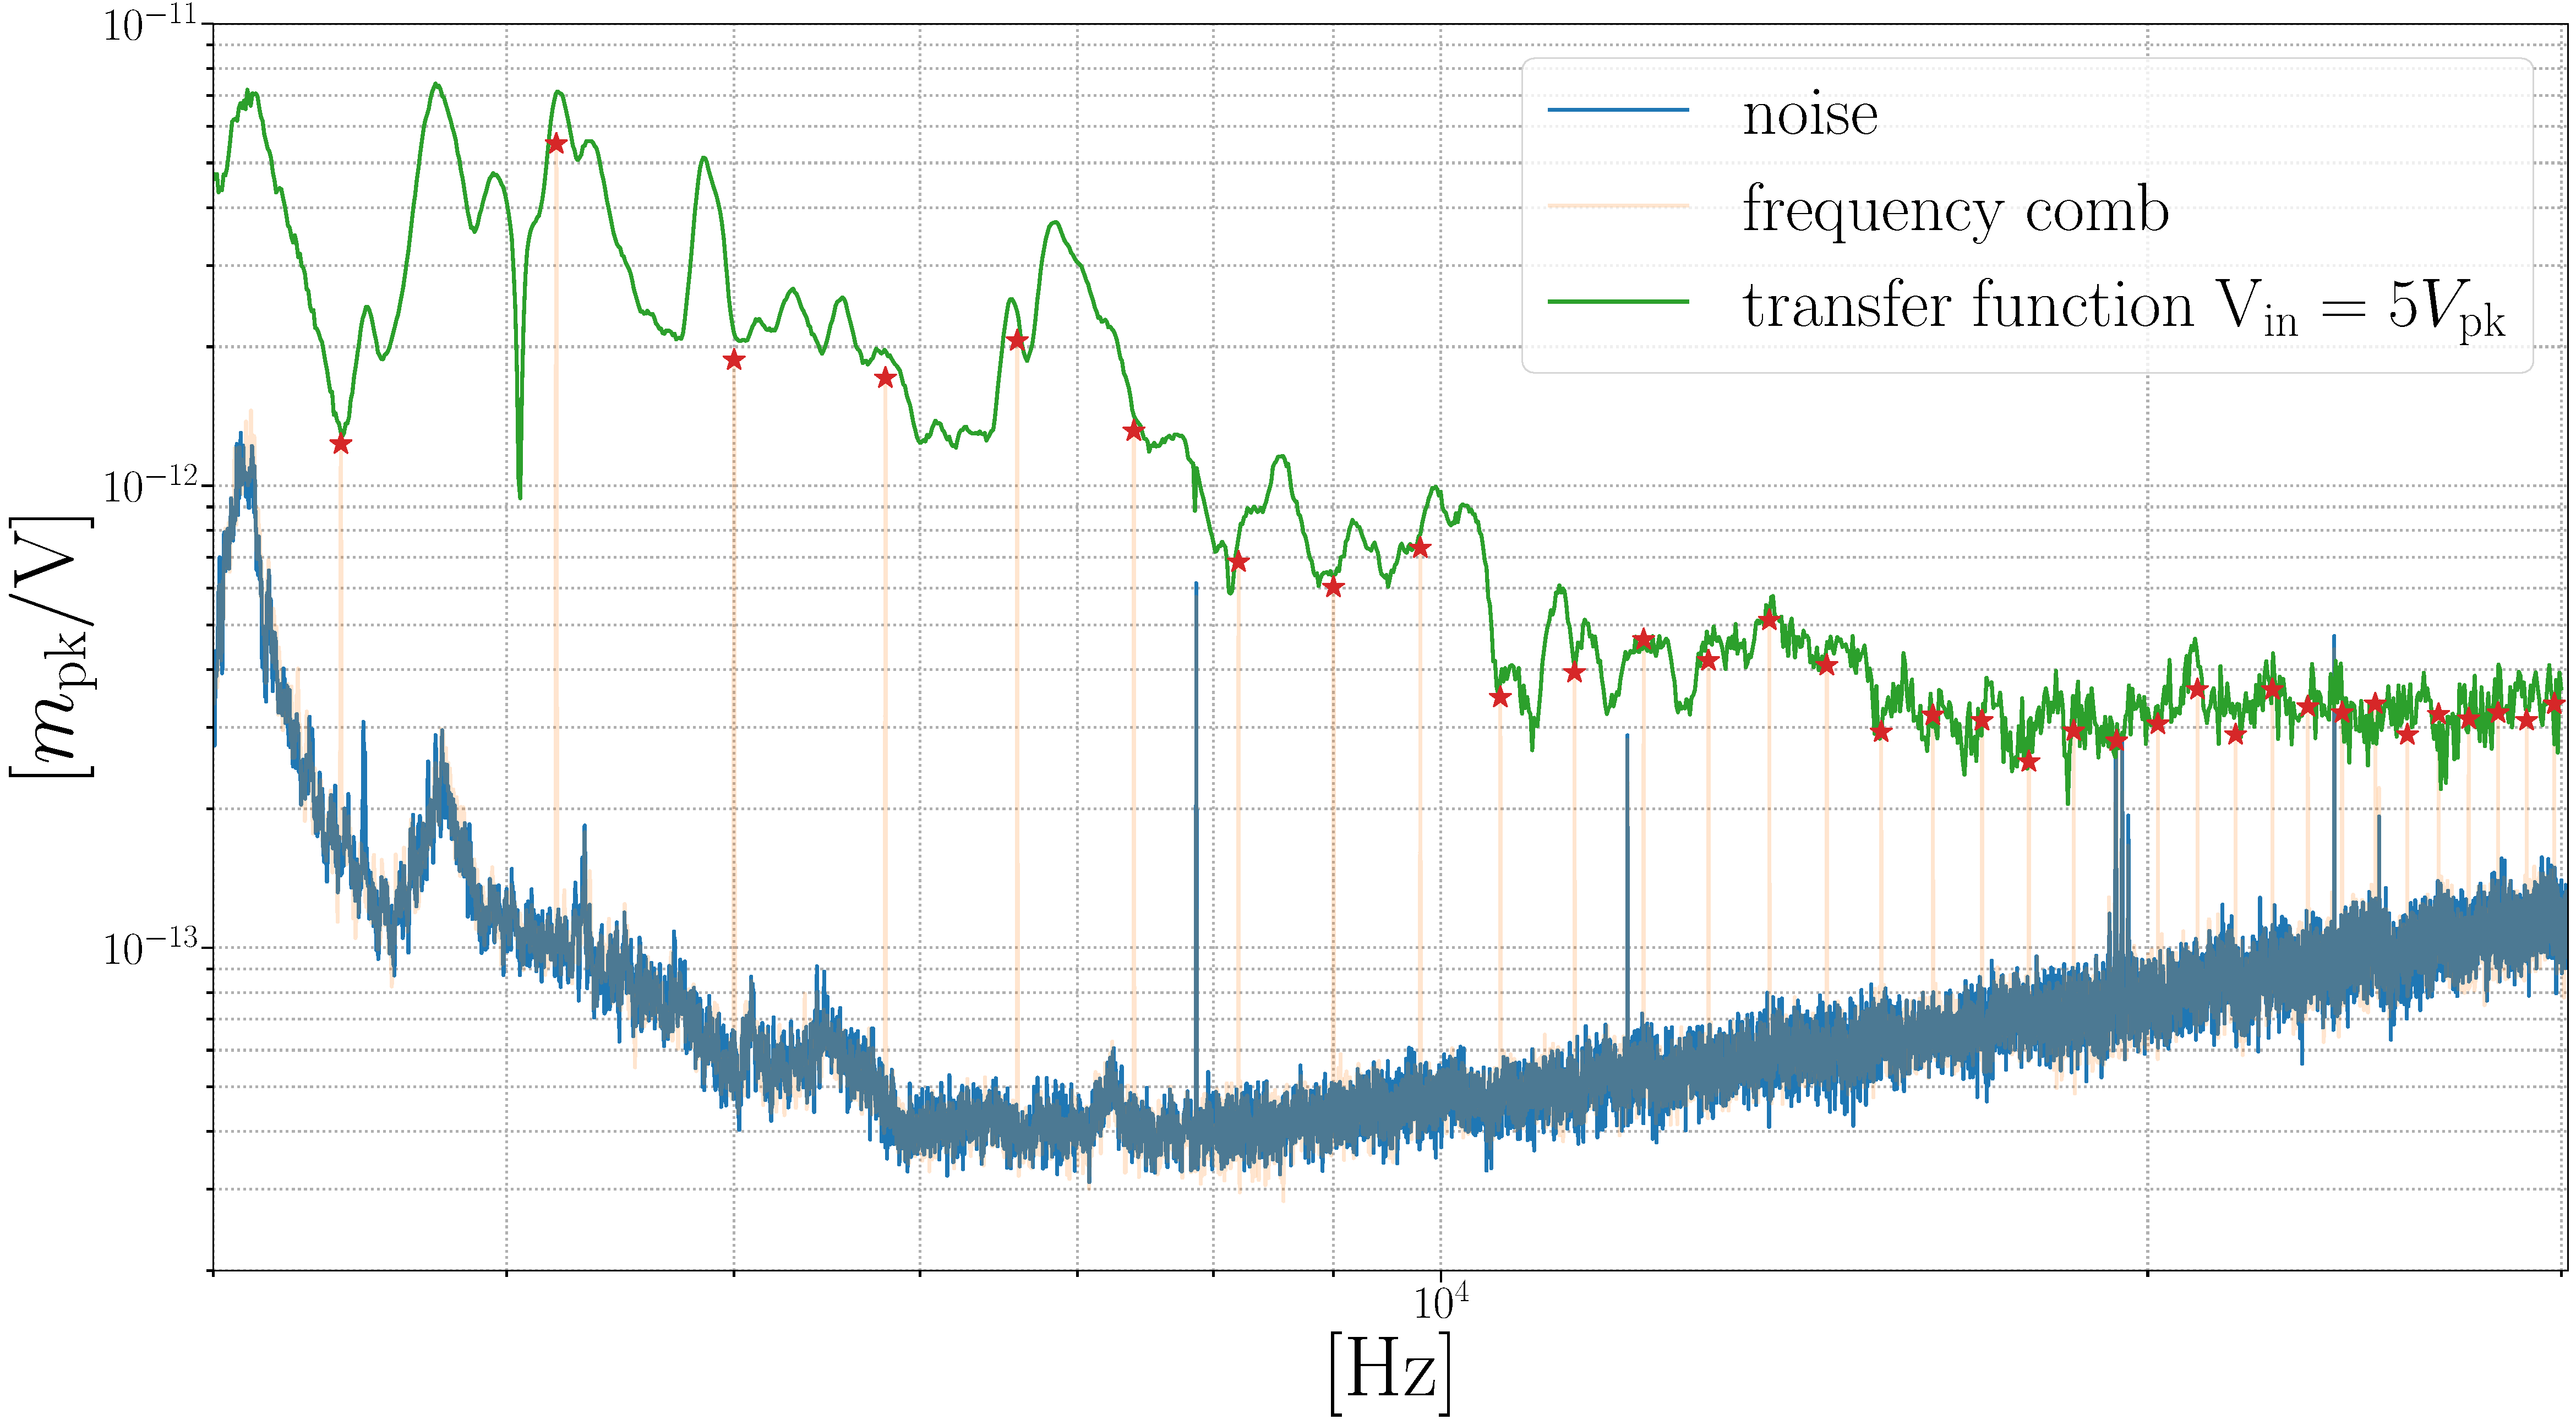
\includegraphics[width=\textwidth]{figs/ALGAAS/results_figs/assembly1/1_2_algaas_tfwcmb.pdf}
    \caption{Assembly 1.2 and 1.3 transfer function measurement and separate noise displacement spectra measurement with the $\gaas$/$\algaas$ sample installed. Measurements were taken from 3kHz up to 21kHz on using a Stanford Research 785 spectrum analyzer.}
    \label{fig:assembly1_2_and_1_3_displacement_spectra_algaas}
\end{figure}

\begin{figure}[H]
    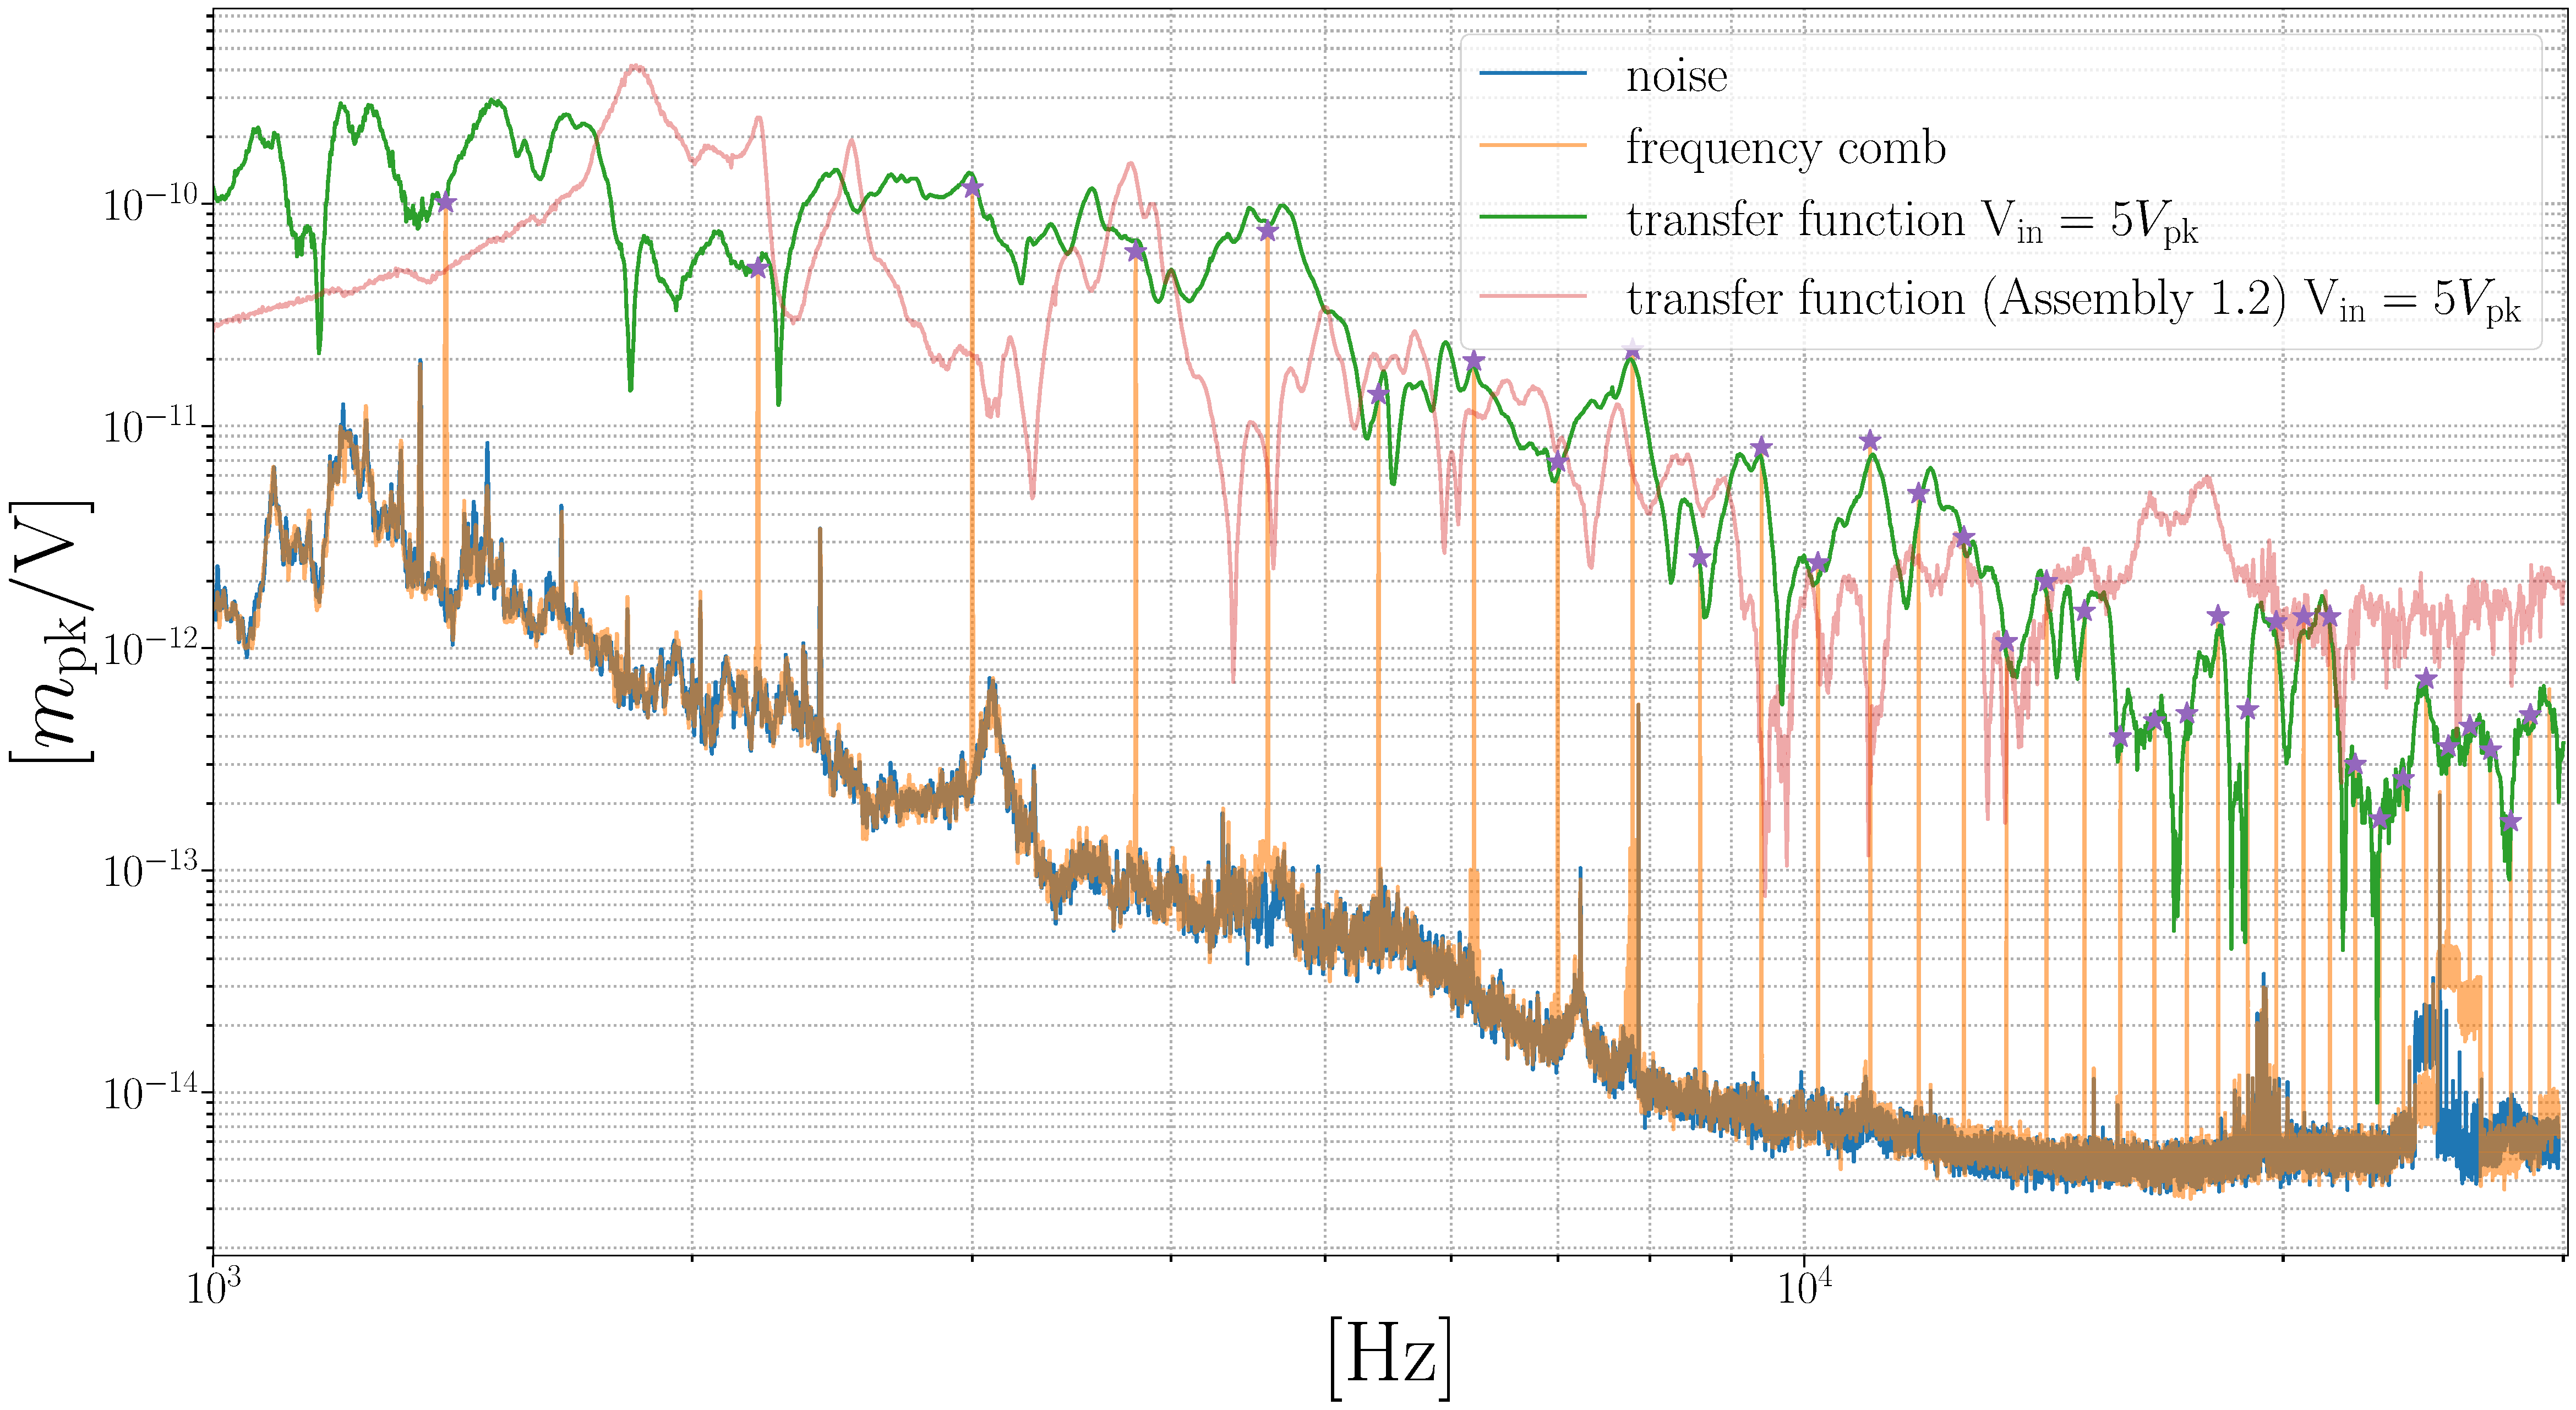
\includegraphics[width=\textwidth]{figs/ALGAAS/results_figs/assembly1/1_2_cvi_compare_tfwcmb.pdf}
    \caption{Assembly 1.2 and 1.3 transfer function measurement and separate noise displacement spectra measurement with a CVI Melles Griot flat mirror sample ($R \approx $ sample installed. Measurements were taken from 1kHz up to 30kHz on using a Stanford Research 785 spectrum analyzer.}
    \label{fig:assembly1_2_and_1_3_displacement_spectra_cvi}
\end{figure}

\subsubsection{Assembly 2}

With considerations after Assembly 1, a more monolithic optical mount design with a simple geometry was imagined. PLA material compliance factoring to the seen drive noise. To see if it could be due to the compliance of the assembly material or printing, we tested this assembly design against different infills of PLA, PETG, and a version machined from solid PVC. With this modification, came also a different plate geometry. The assumption is the region of interest of the injection would not be heavily influenced by the non-circular plate geometry where it matters.

% Some citations:
%\cite{PINTO2015635}

%\begin{figure}[!ht]
%	\begin{subcaptiongroup}
%		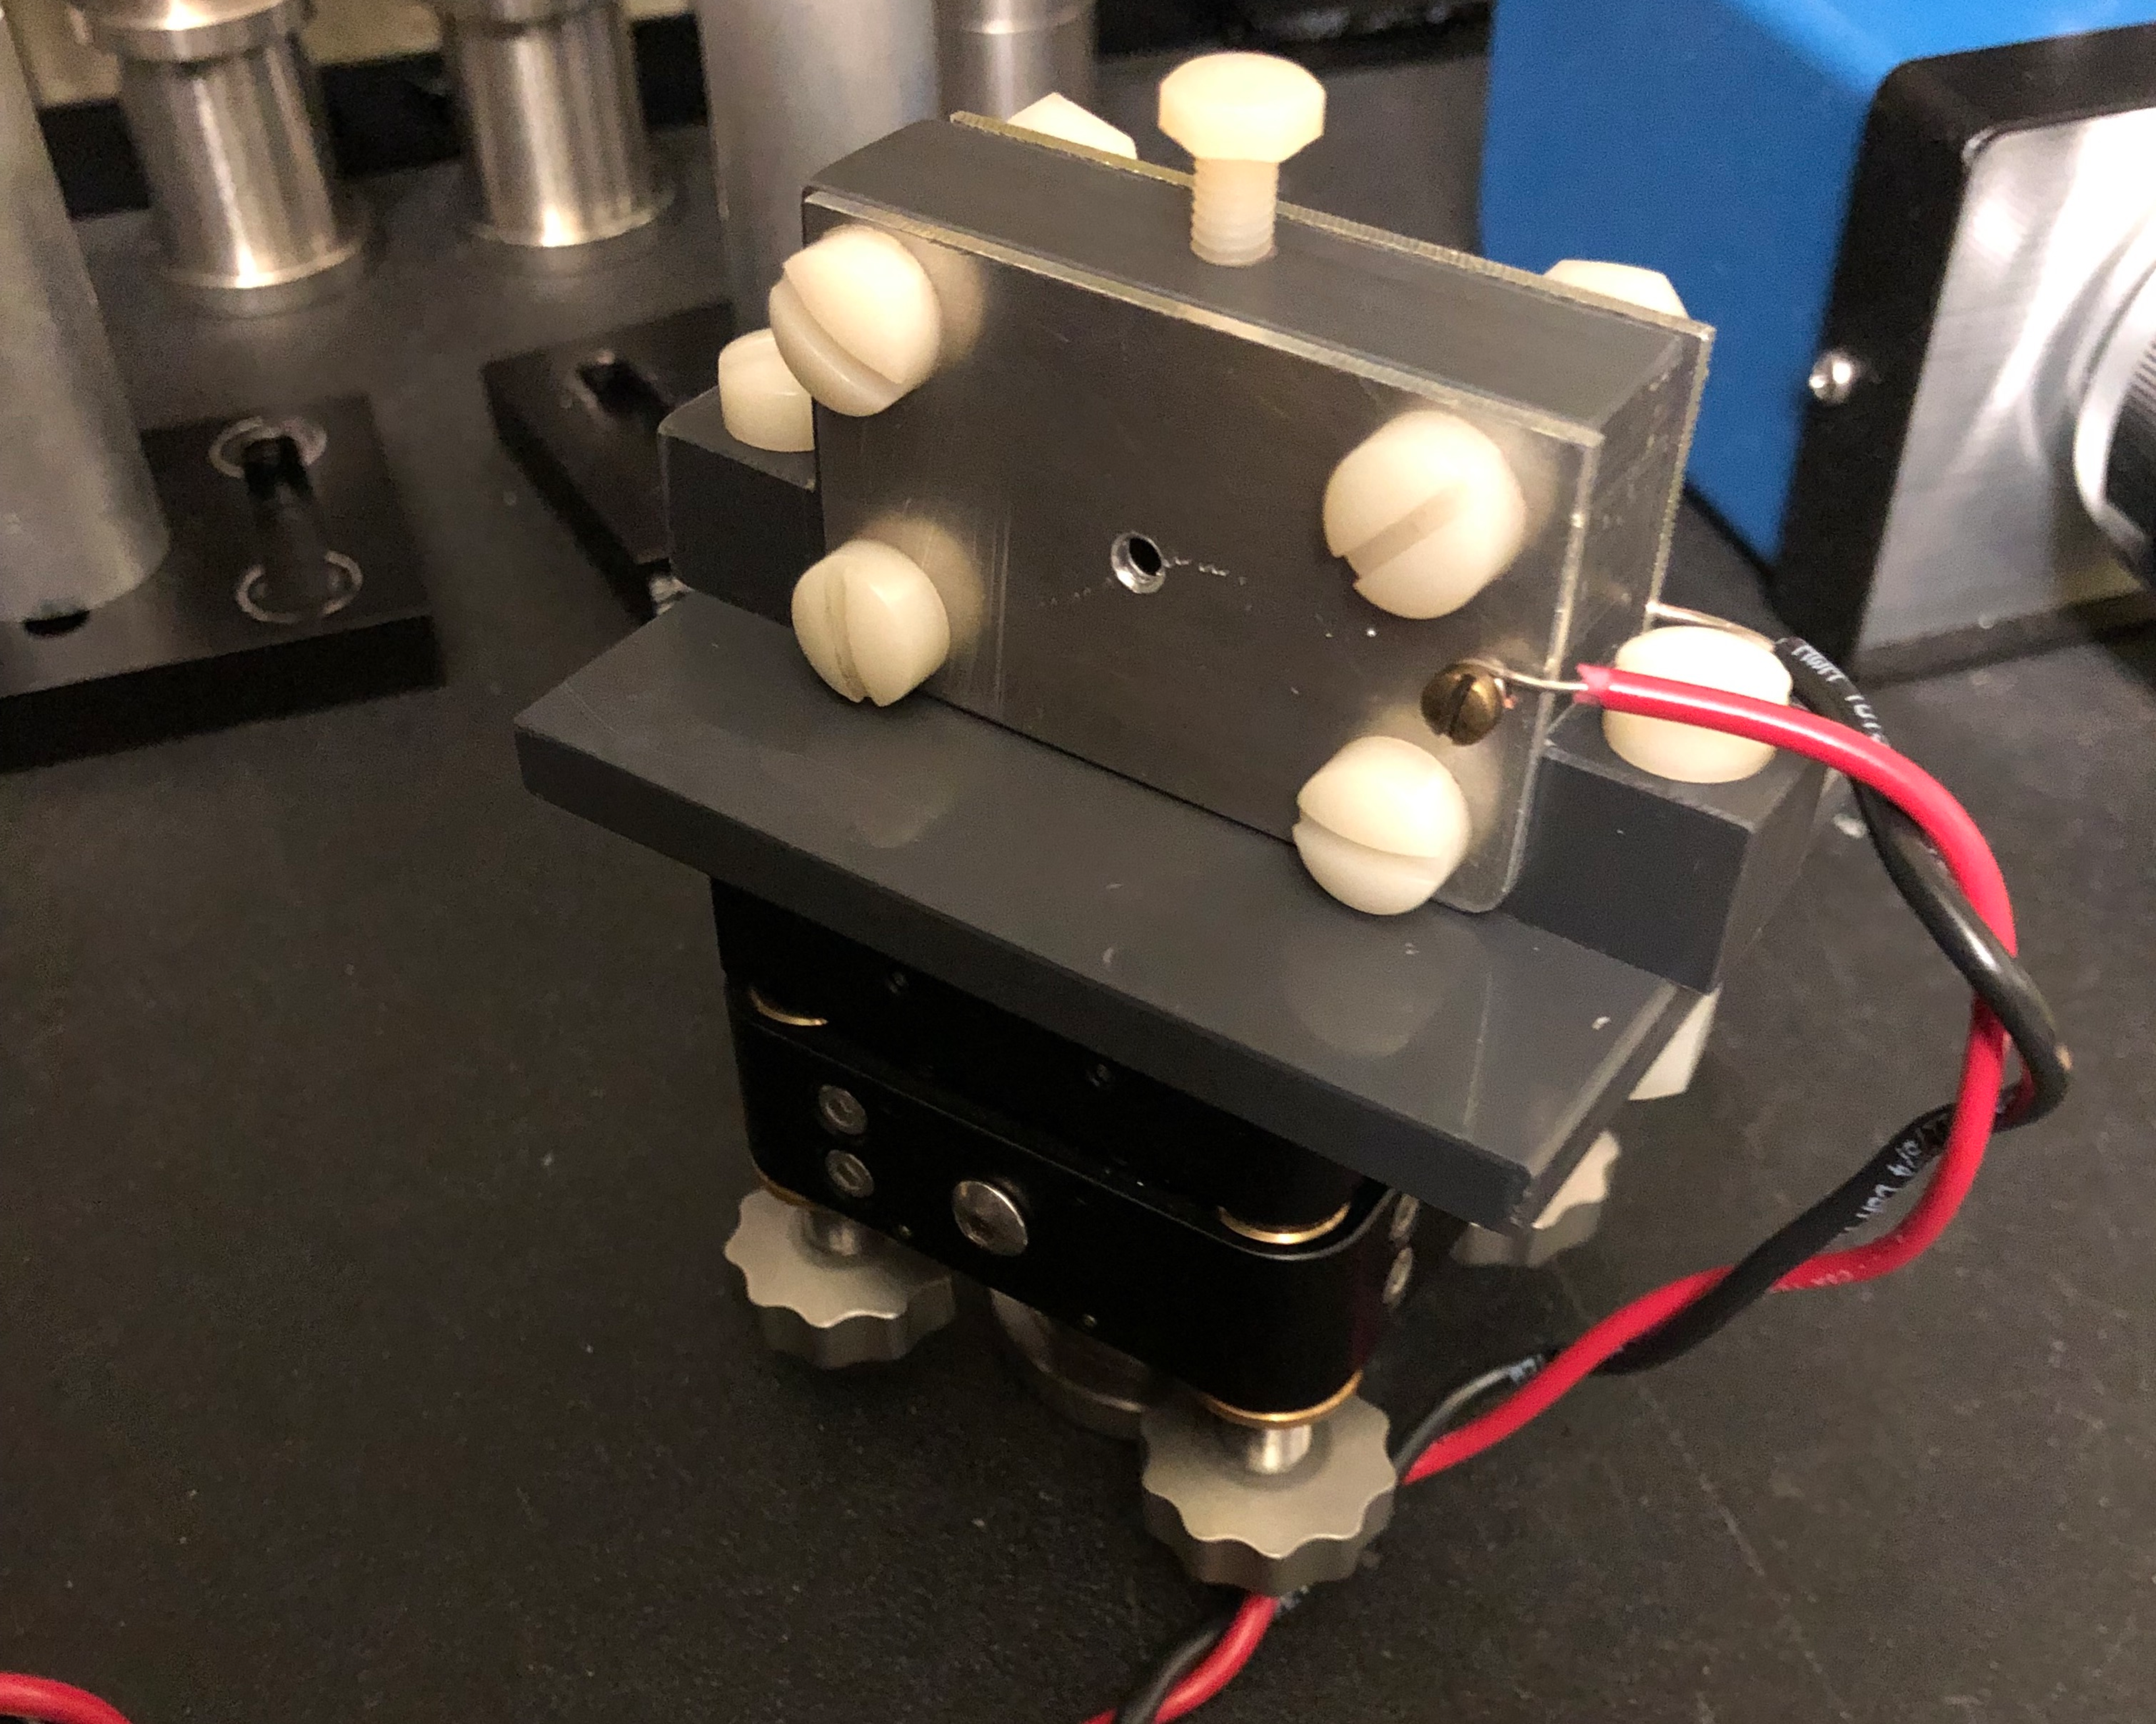
\includegraphics[width=.5\textwidth]{figs/ALGAAS/assemblies/assembly2/assembly2_PVC.pdf}
%		\phantomcaption\label{A2_PVC}
%		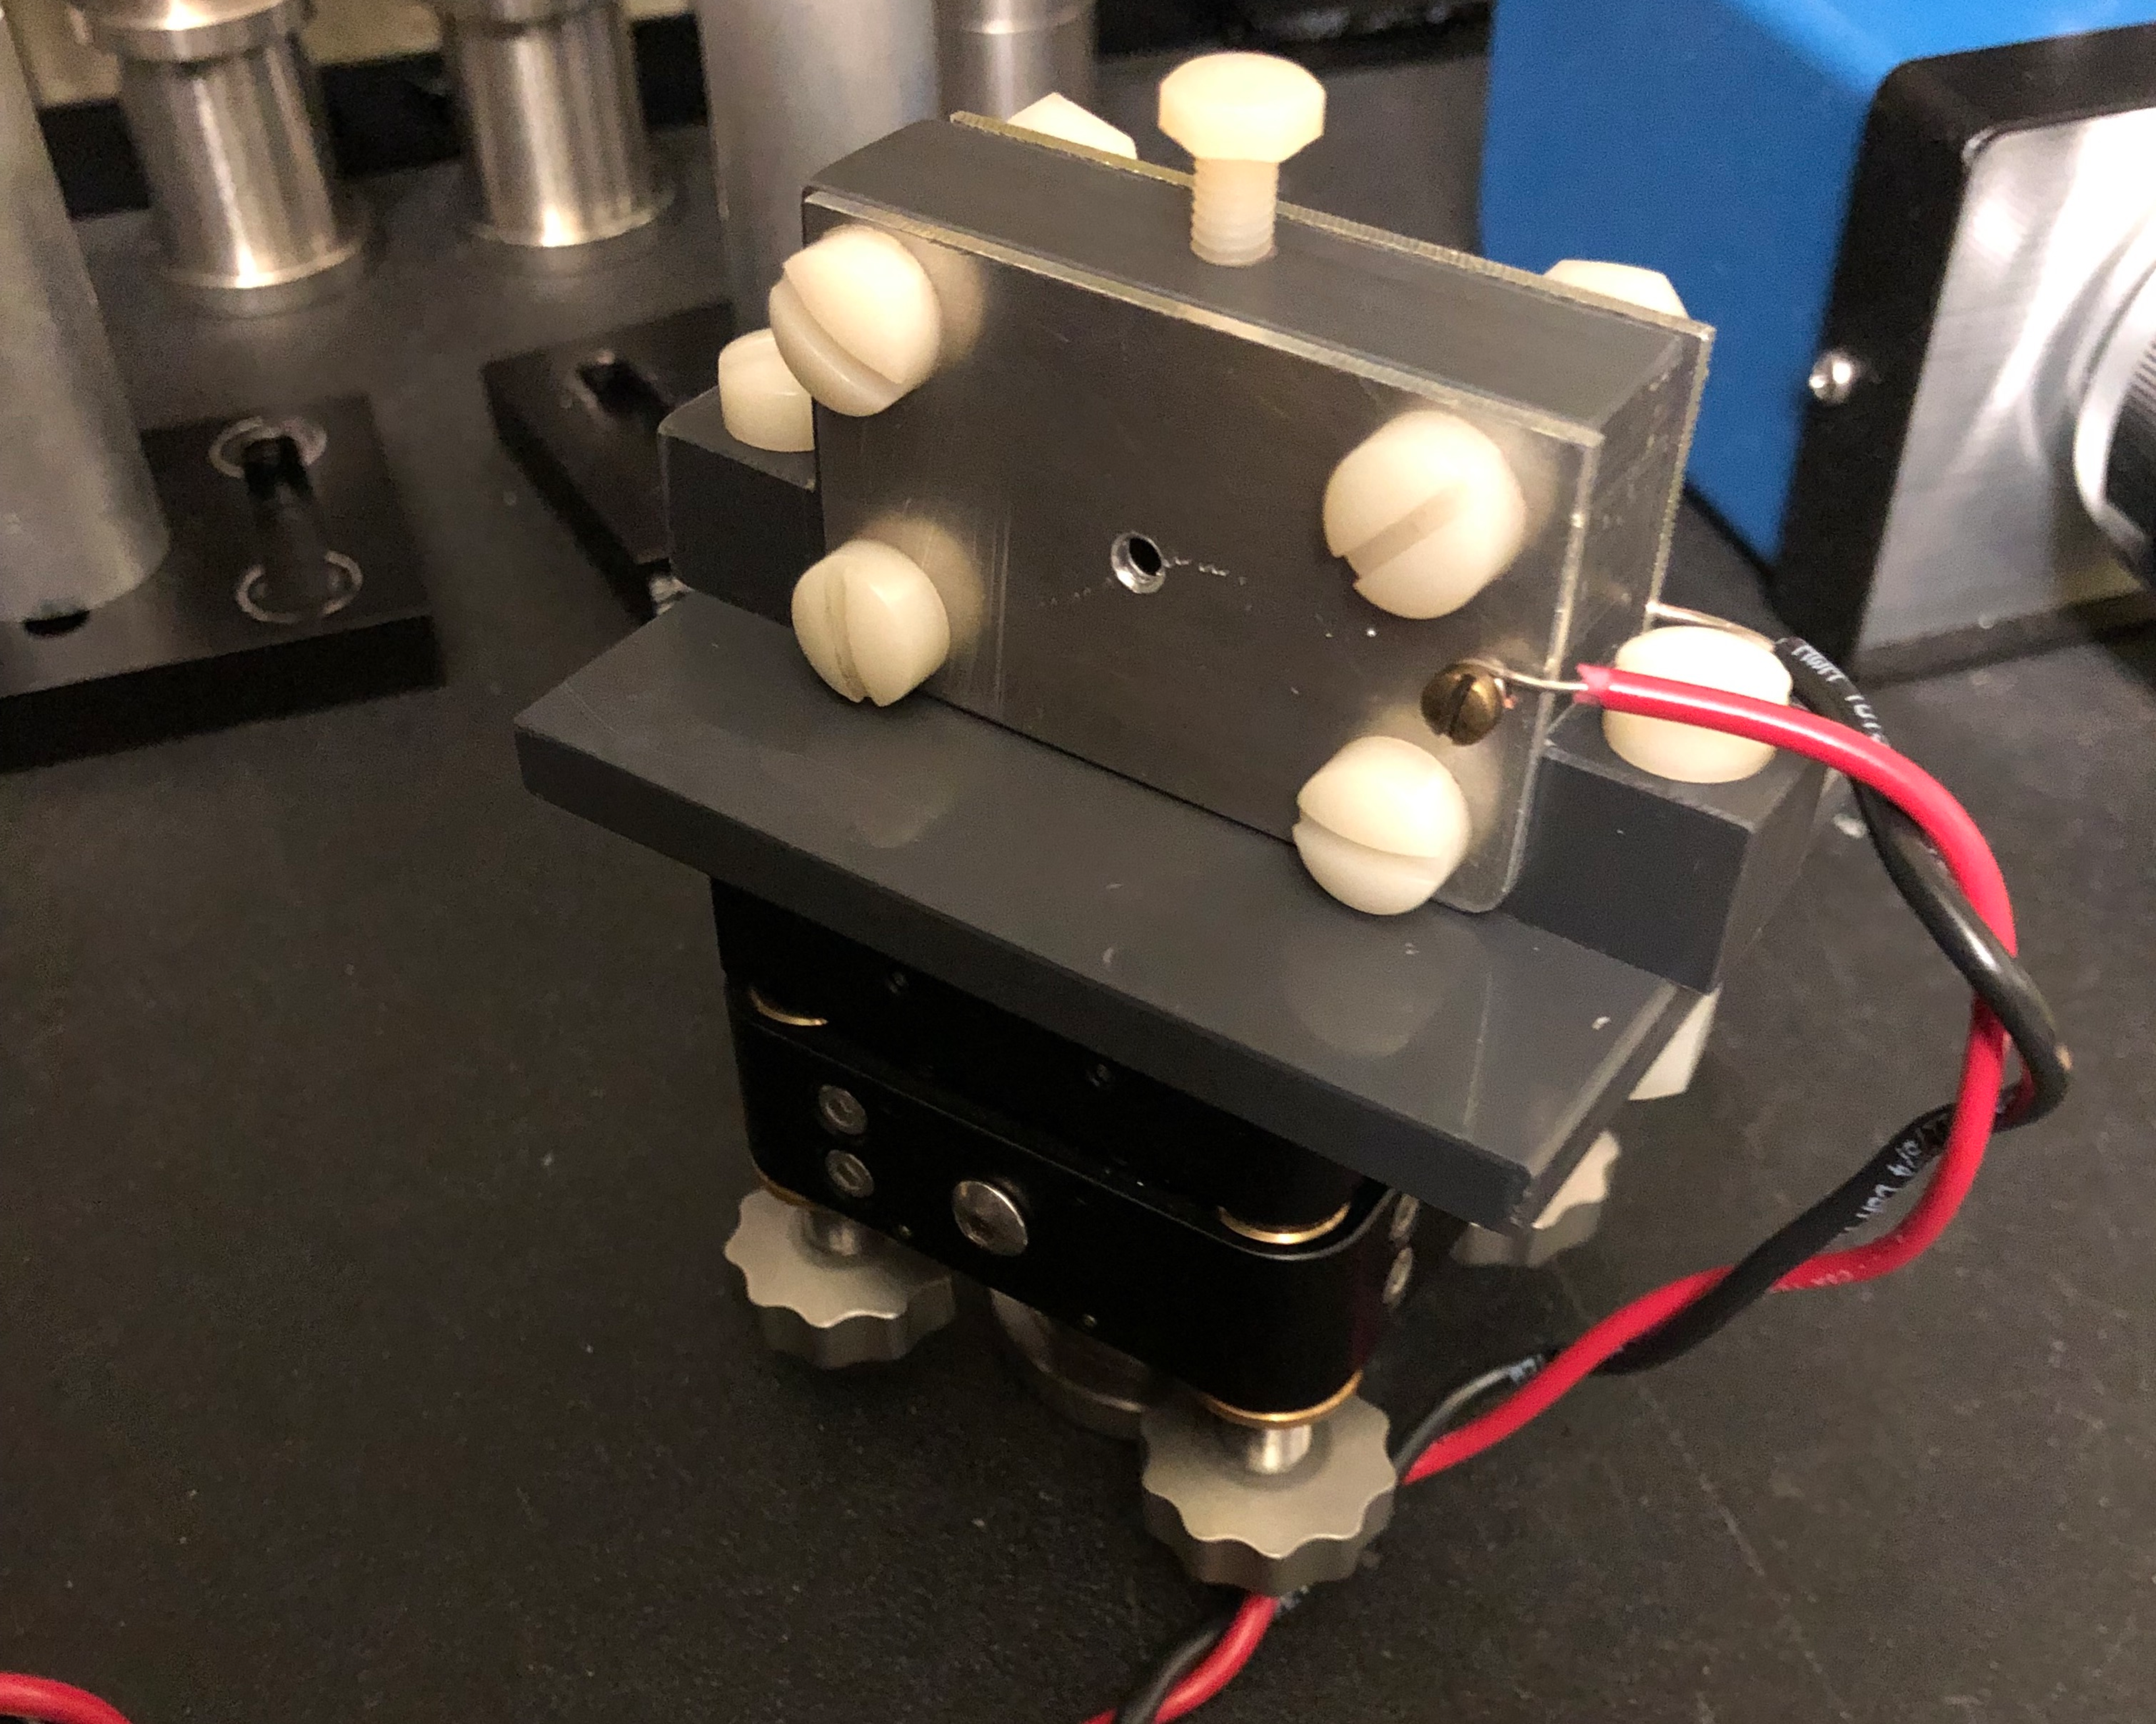
\includegraphics[width=.5\textwidth]{figs/ALGAAS/assemblies/assembly2/assembly2_PVC.pdf}
%		\phantomcaption\label{A2_PVC}
%    	\end{subcaptiongroup}
%    \caption{An iteration of assembly 2 comprised of a PVC mount with two rectangular (1.1"X2") plates with a central aperture of 3mm}
%    \label{fig:assembly2}
%\end{figure}

\begin{figure}[H]
    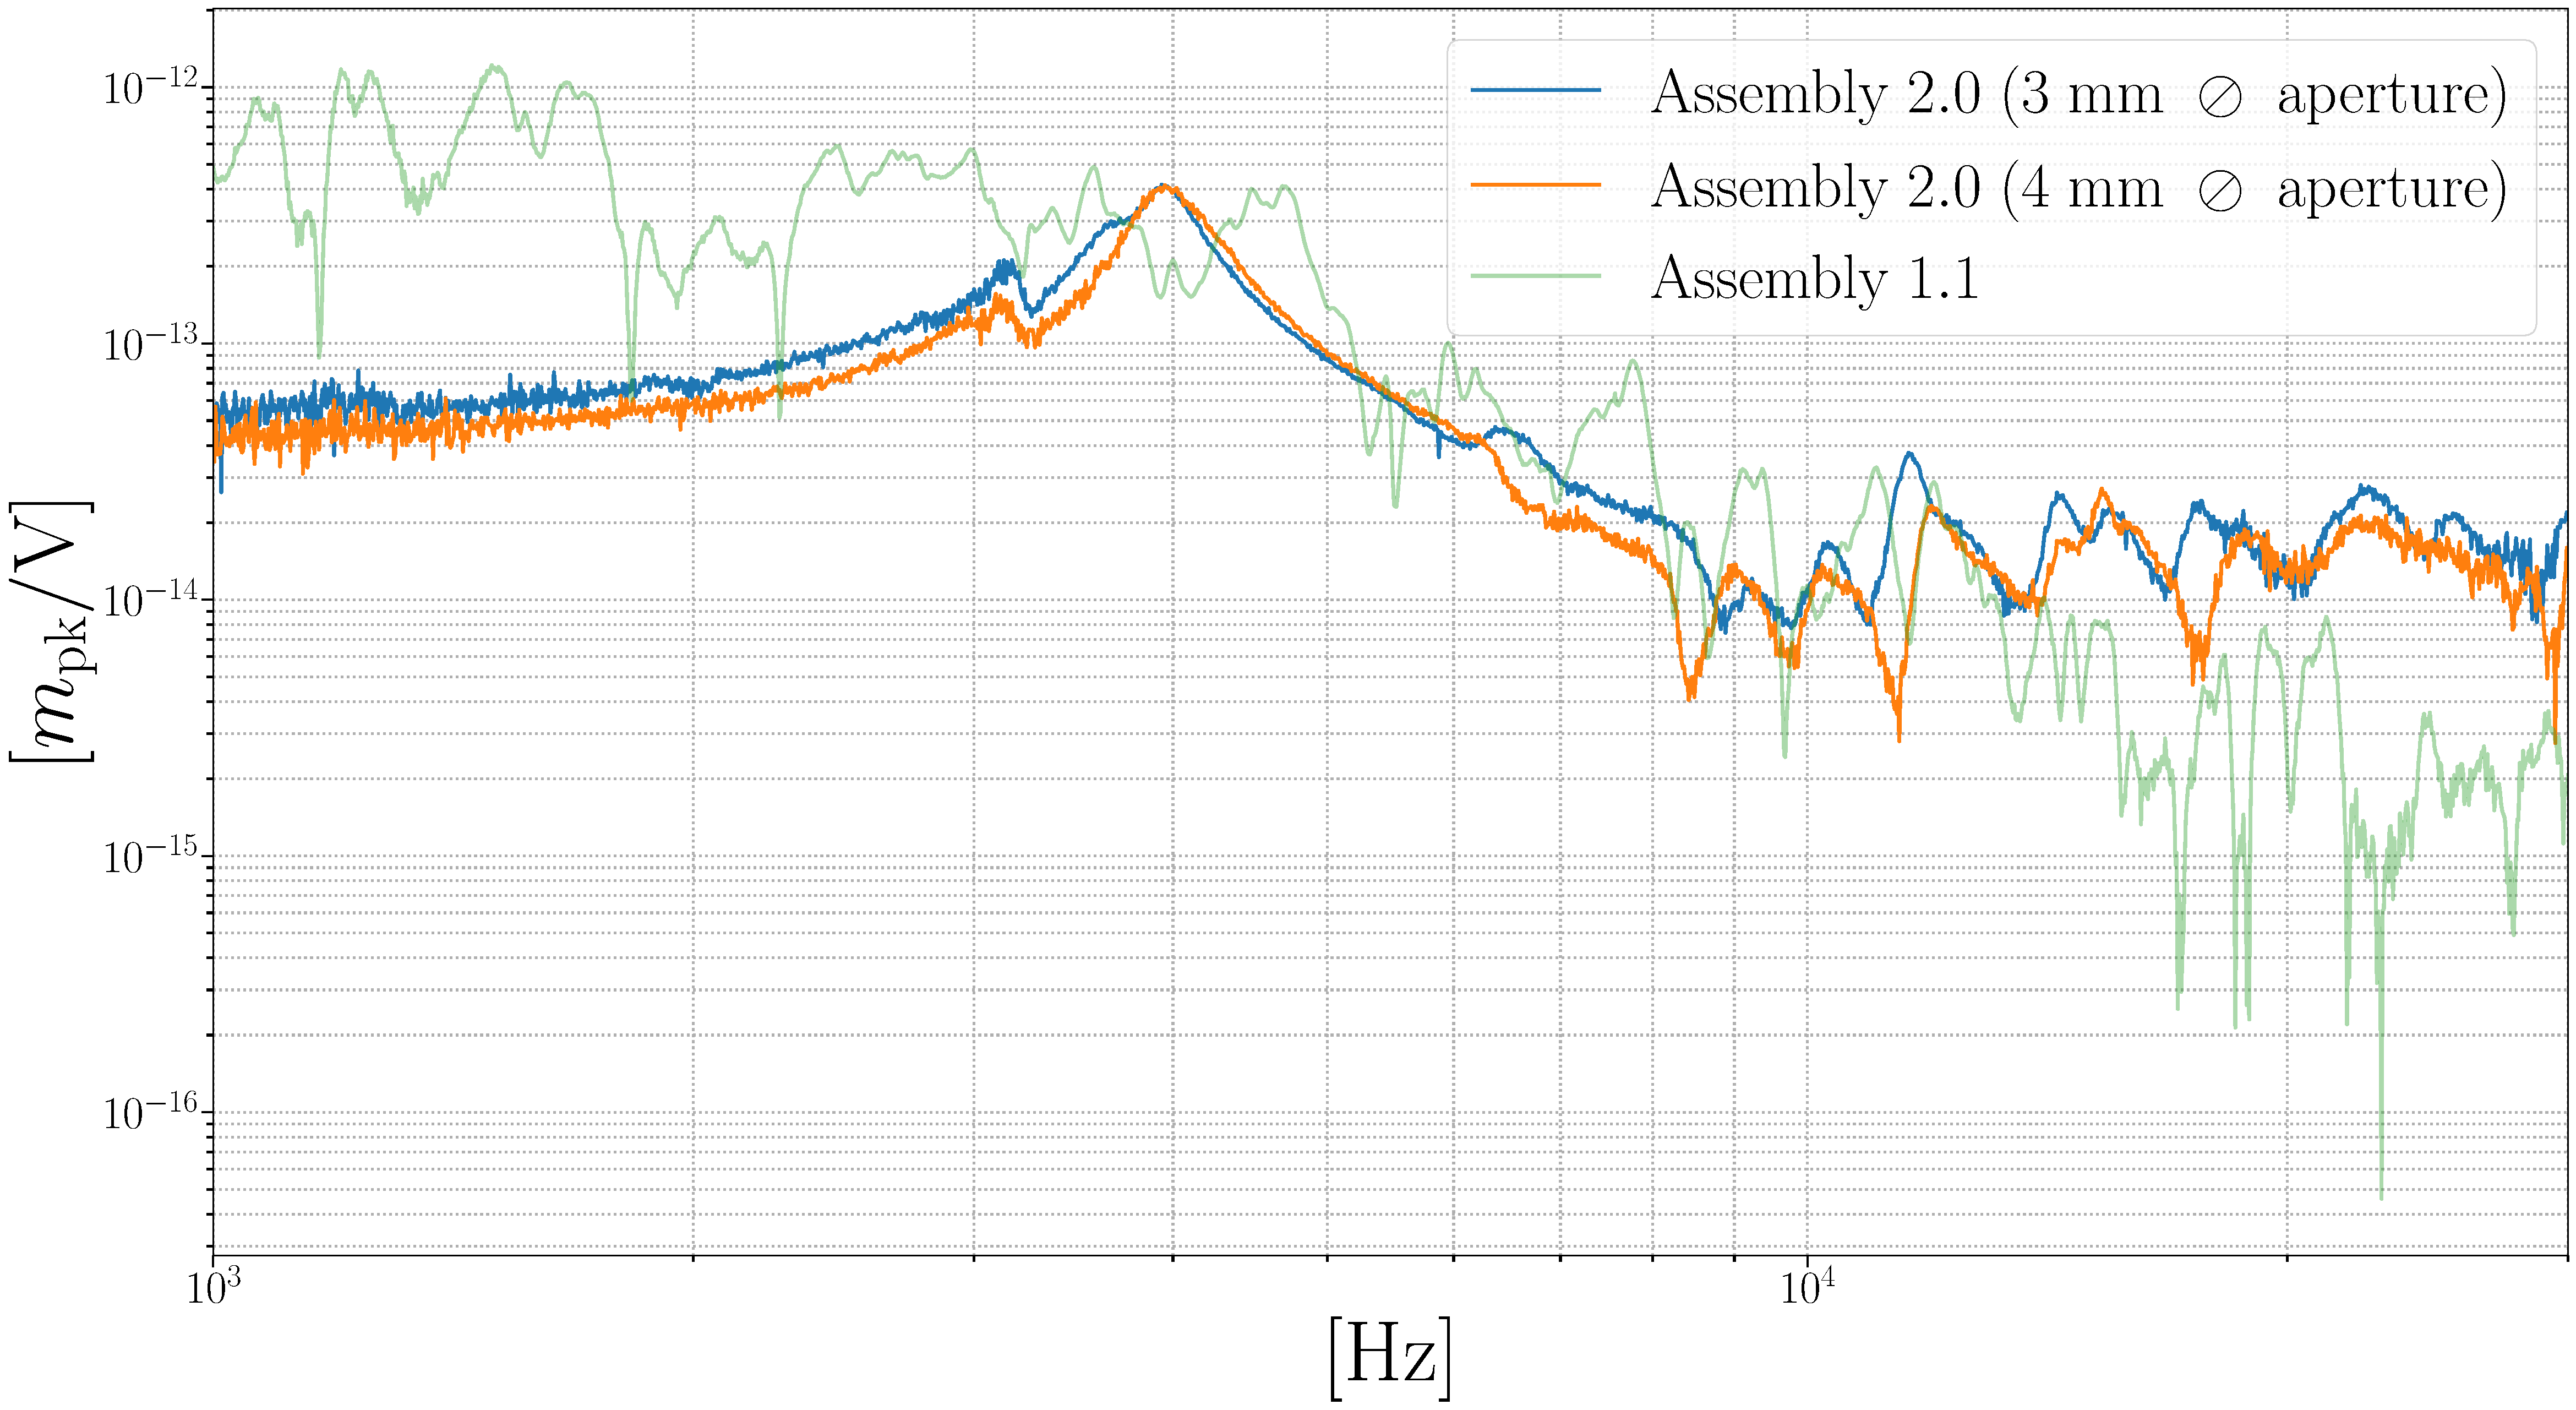
\includegraphics[width=\textwidth]{figs/ALGAAS/results_figs/assembly2/2_0_compare_1_1.pdf} 
    \caption{Assembly 2.0 transfer function measurements compared to Assembly 1.1, Measurements were taken from 1kHz up to 30kHz on using a Stanford Research 785 spectrum analyzer.}
    \label{fig:assembly2and1_1}
\end{figure}


\begin{figure}[H]
    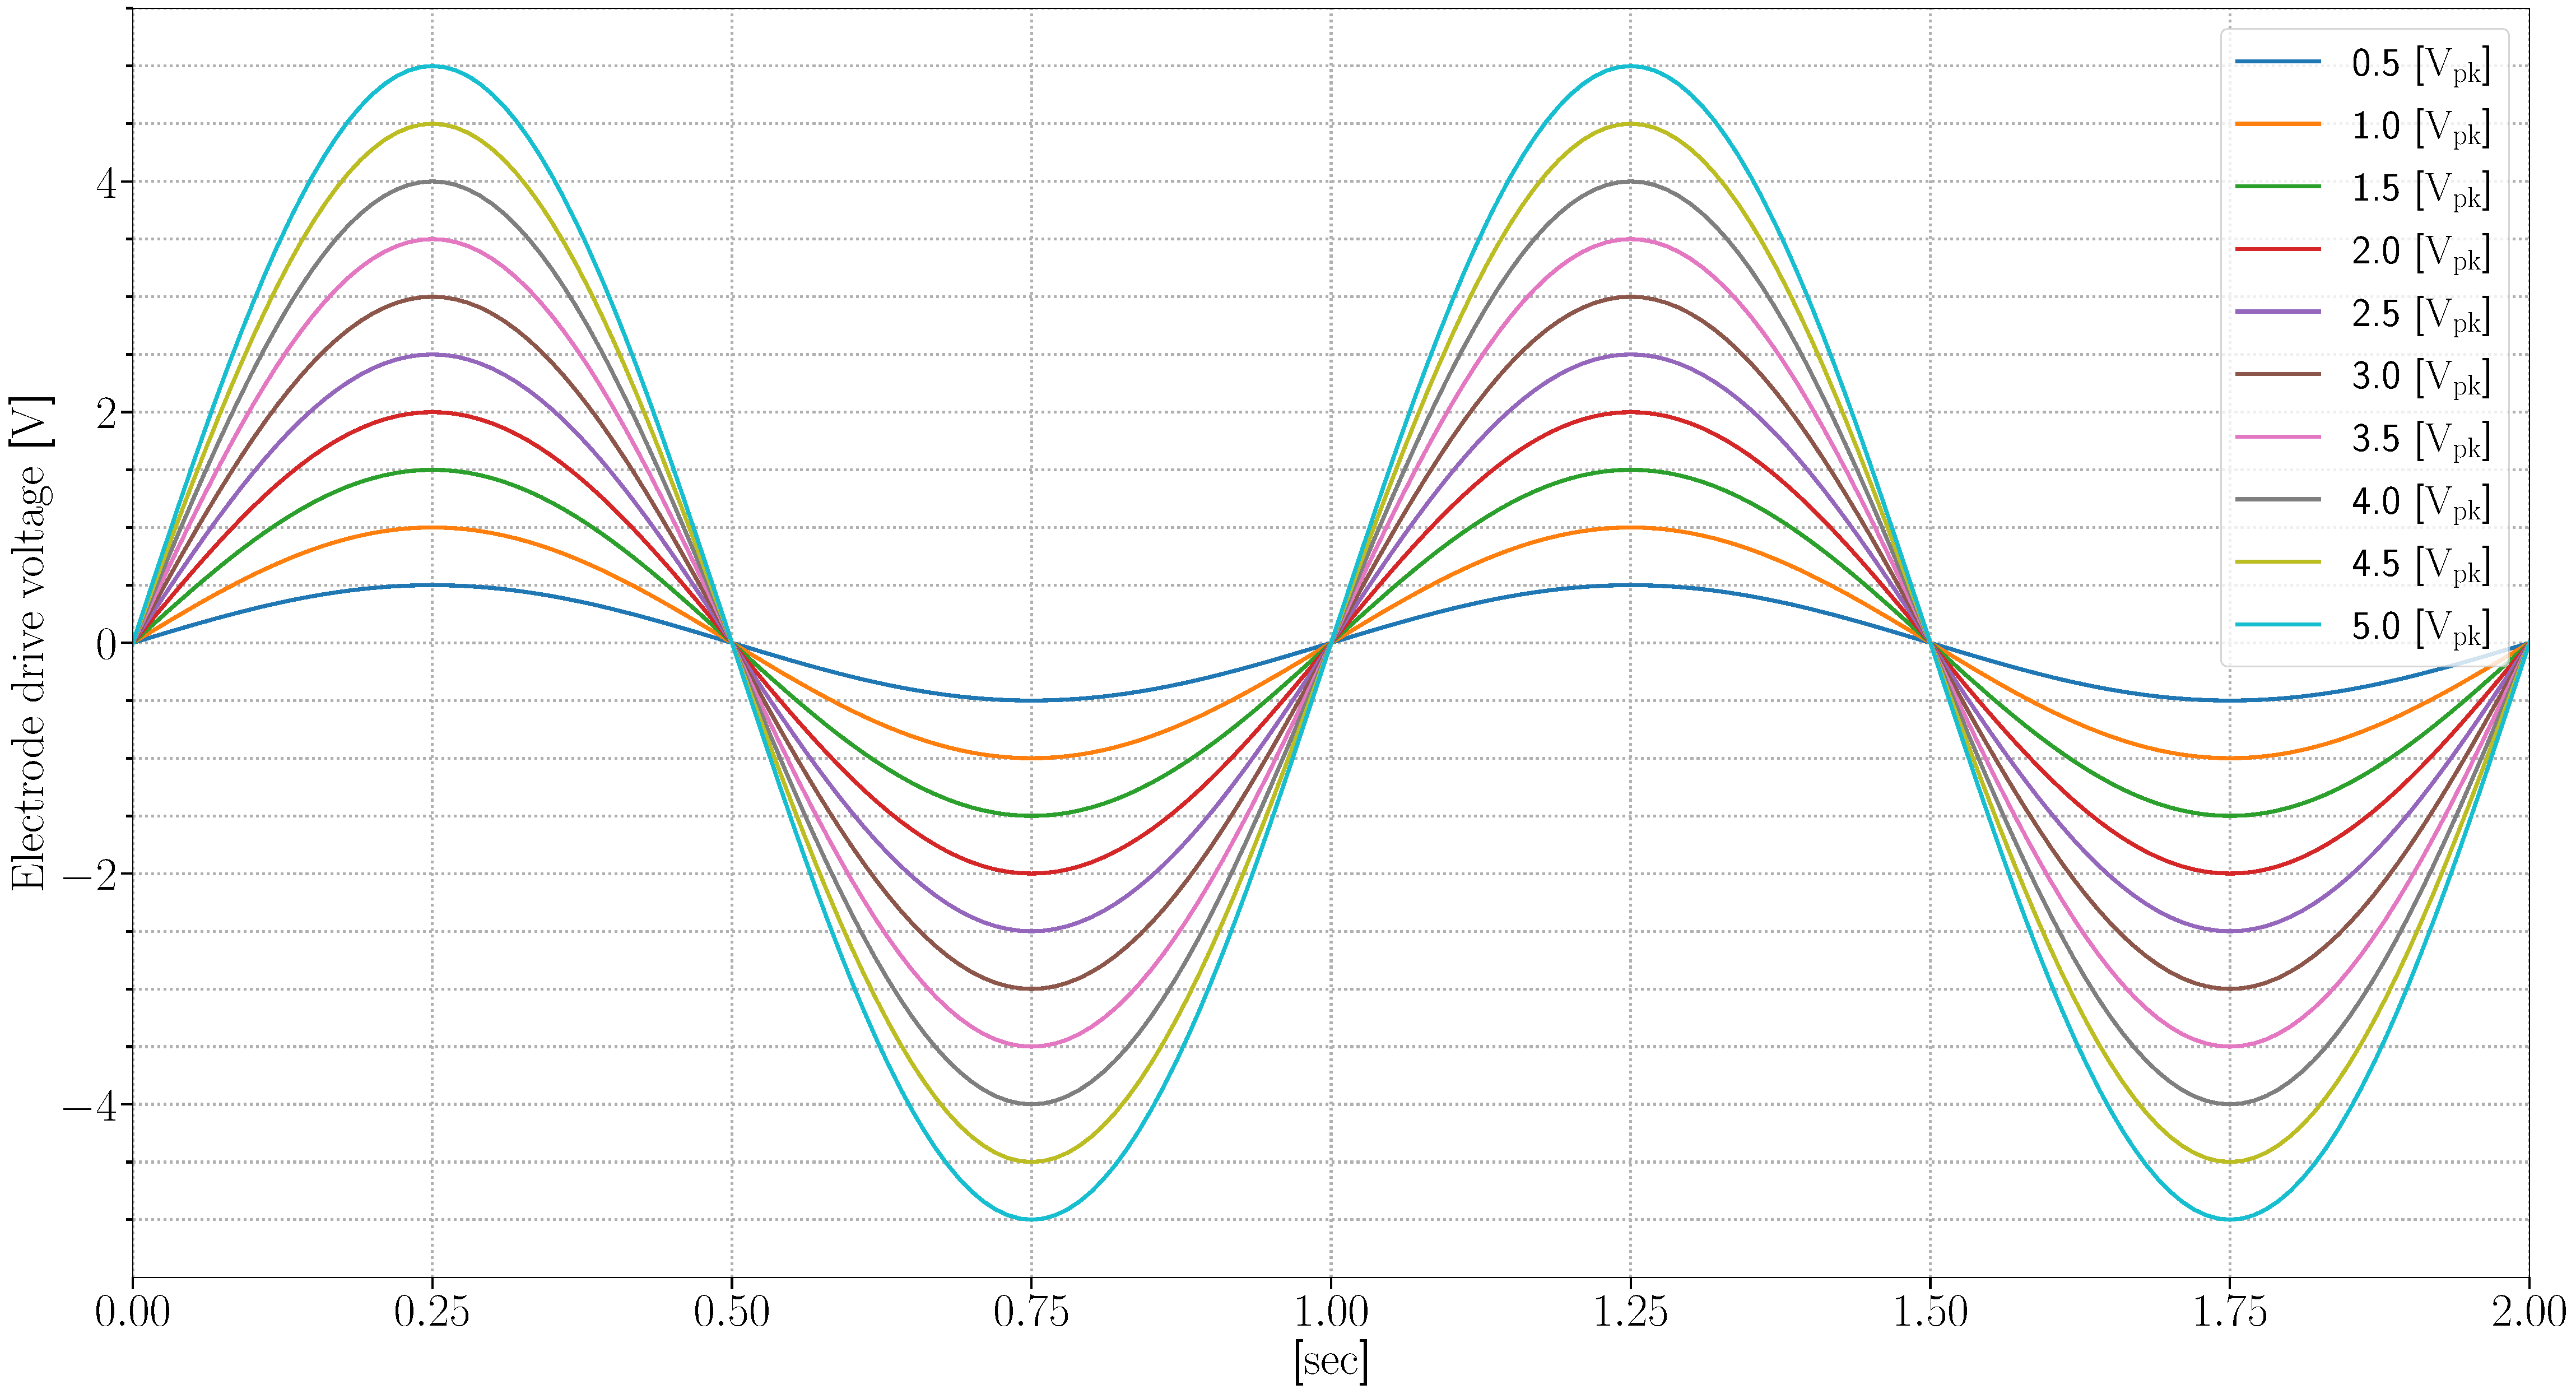
\includegraphics[width=\textwidth]{figs/ALGAAS/results_figs/assembly2/vary_da.pdf}
    \caption{The varied drive amplitudes input into the HVA to perform the following test}
    \label{fig:vary_da}
\end{figure}

\begin{figure}[H]
    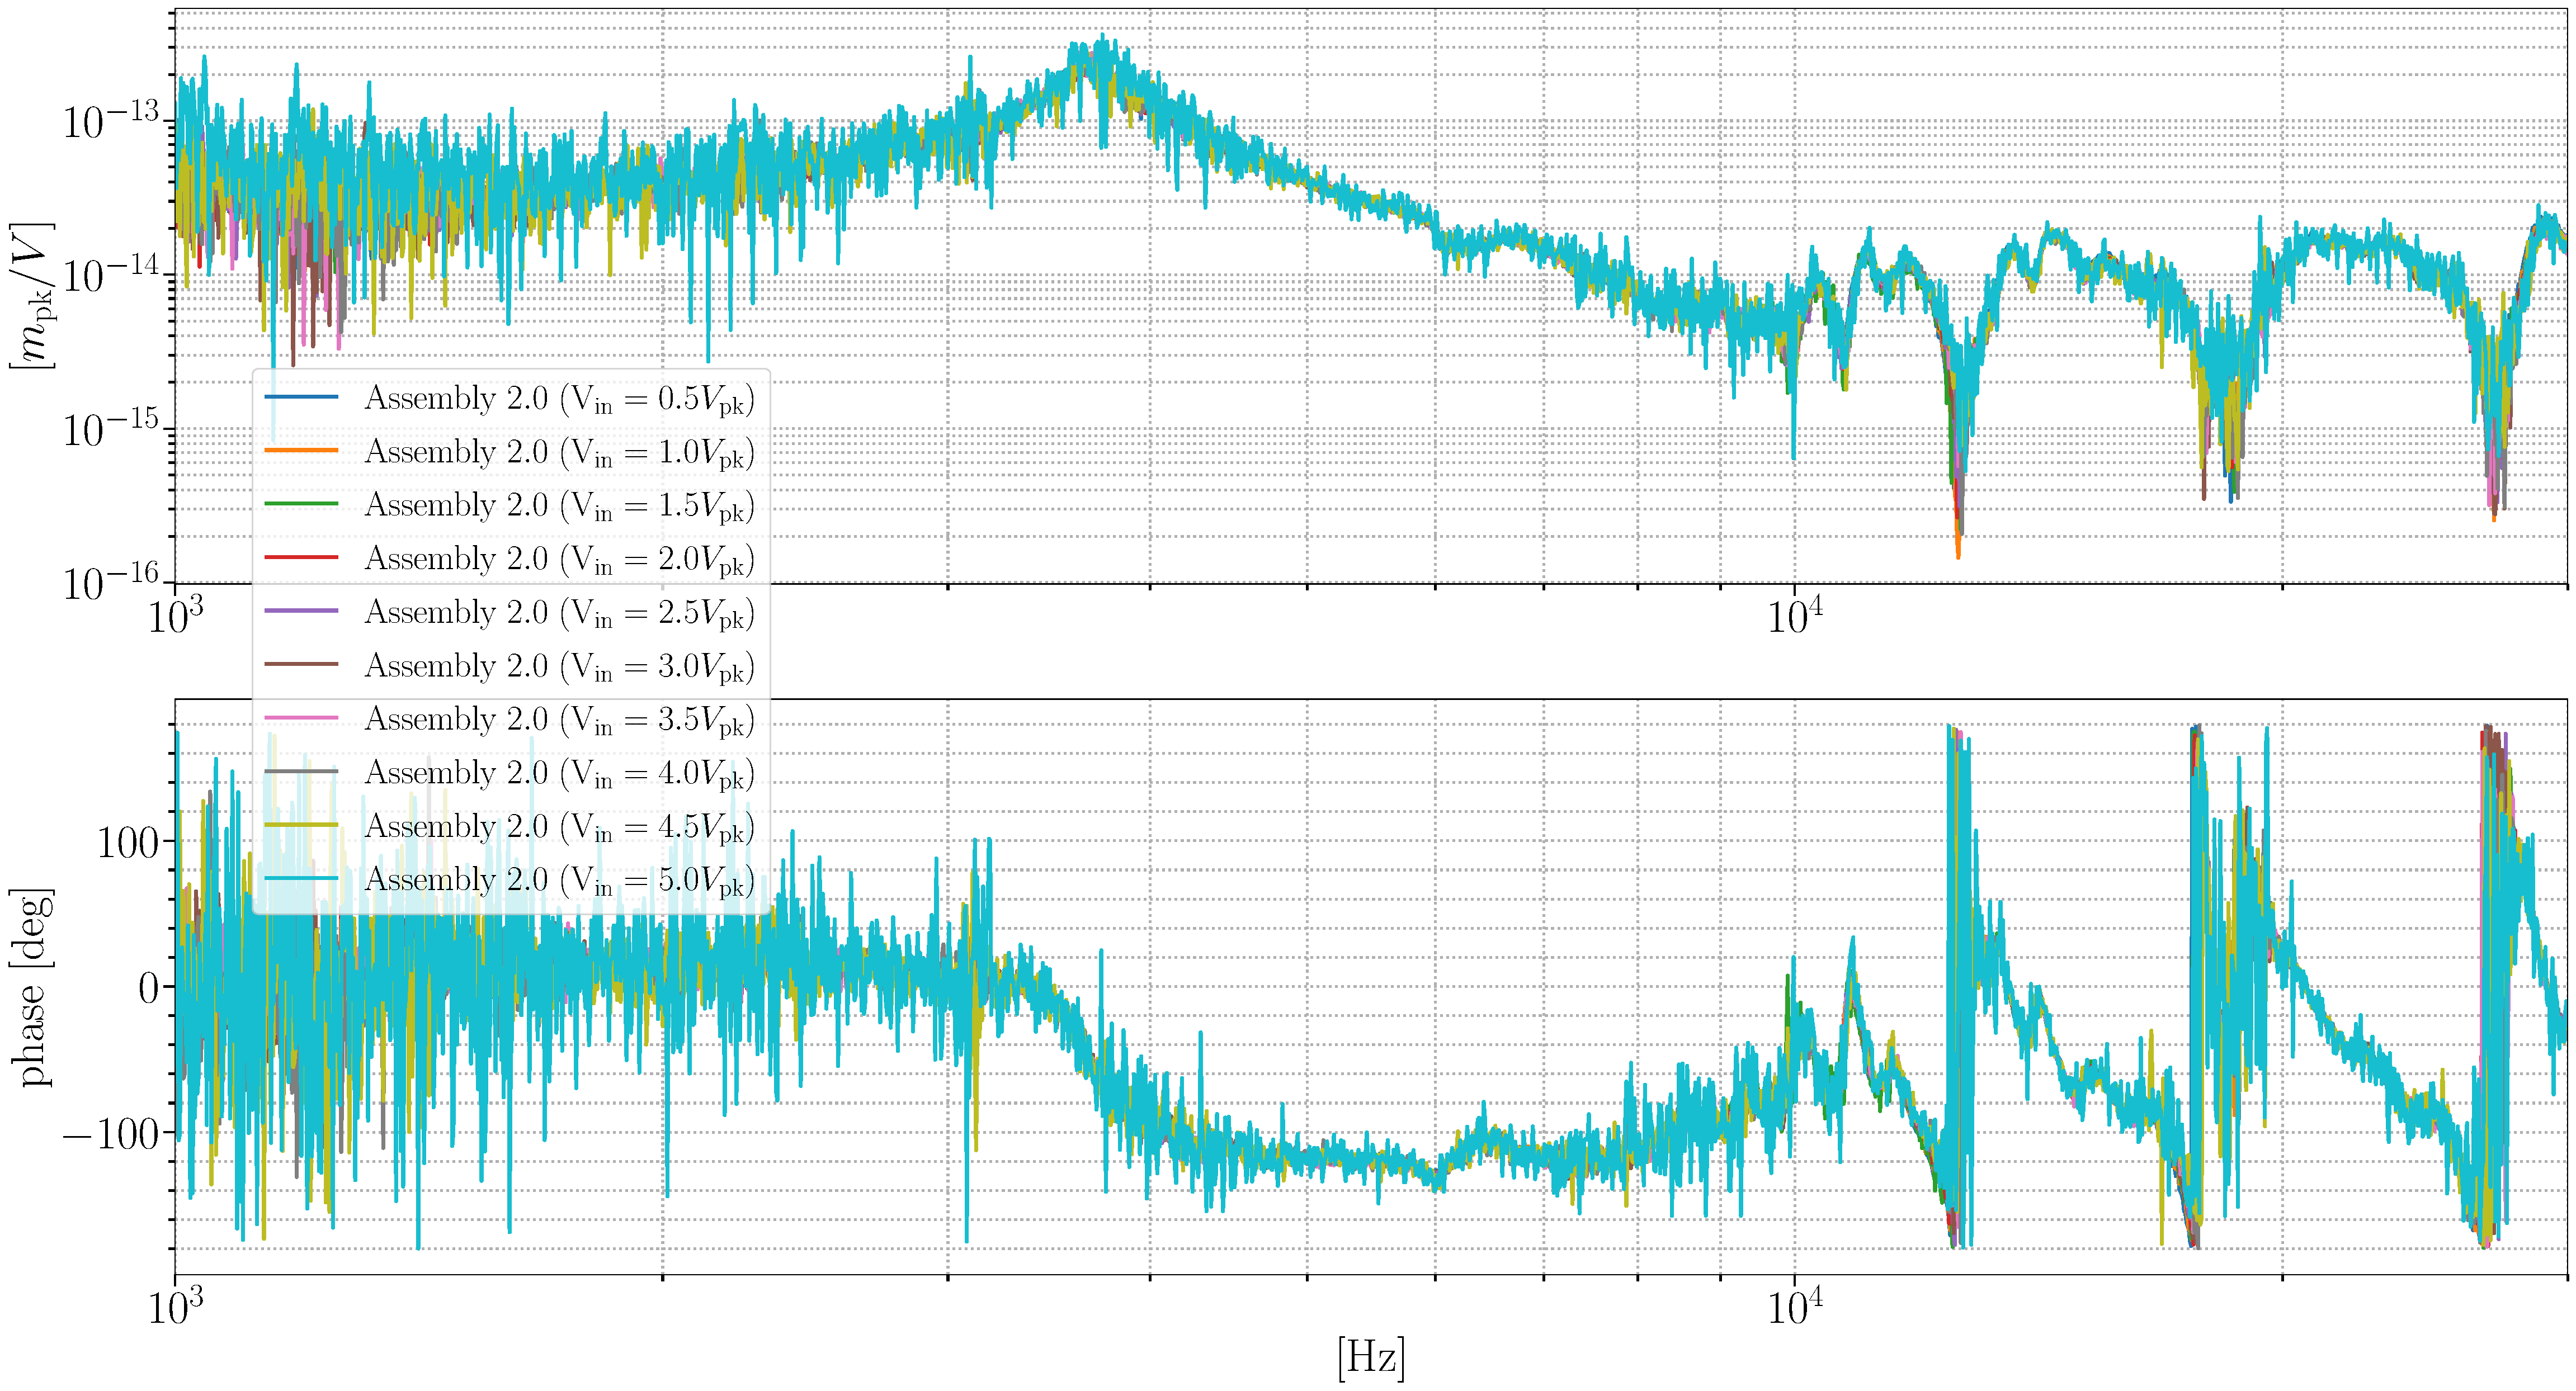
\includegraphics[width=\textwidth]{figs/ALGAAS/results_figs/assembly2/vv53.pdf} 
    \caption{Assembly 2.0 transfer function measurements with varied drive amplitudes indicated in ~\ref{fig:vary_da}.}
    \label{fig:vv53}
\end{figure}


\begin{figure}[H]
    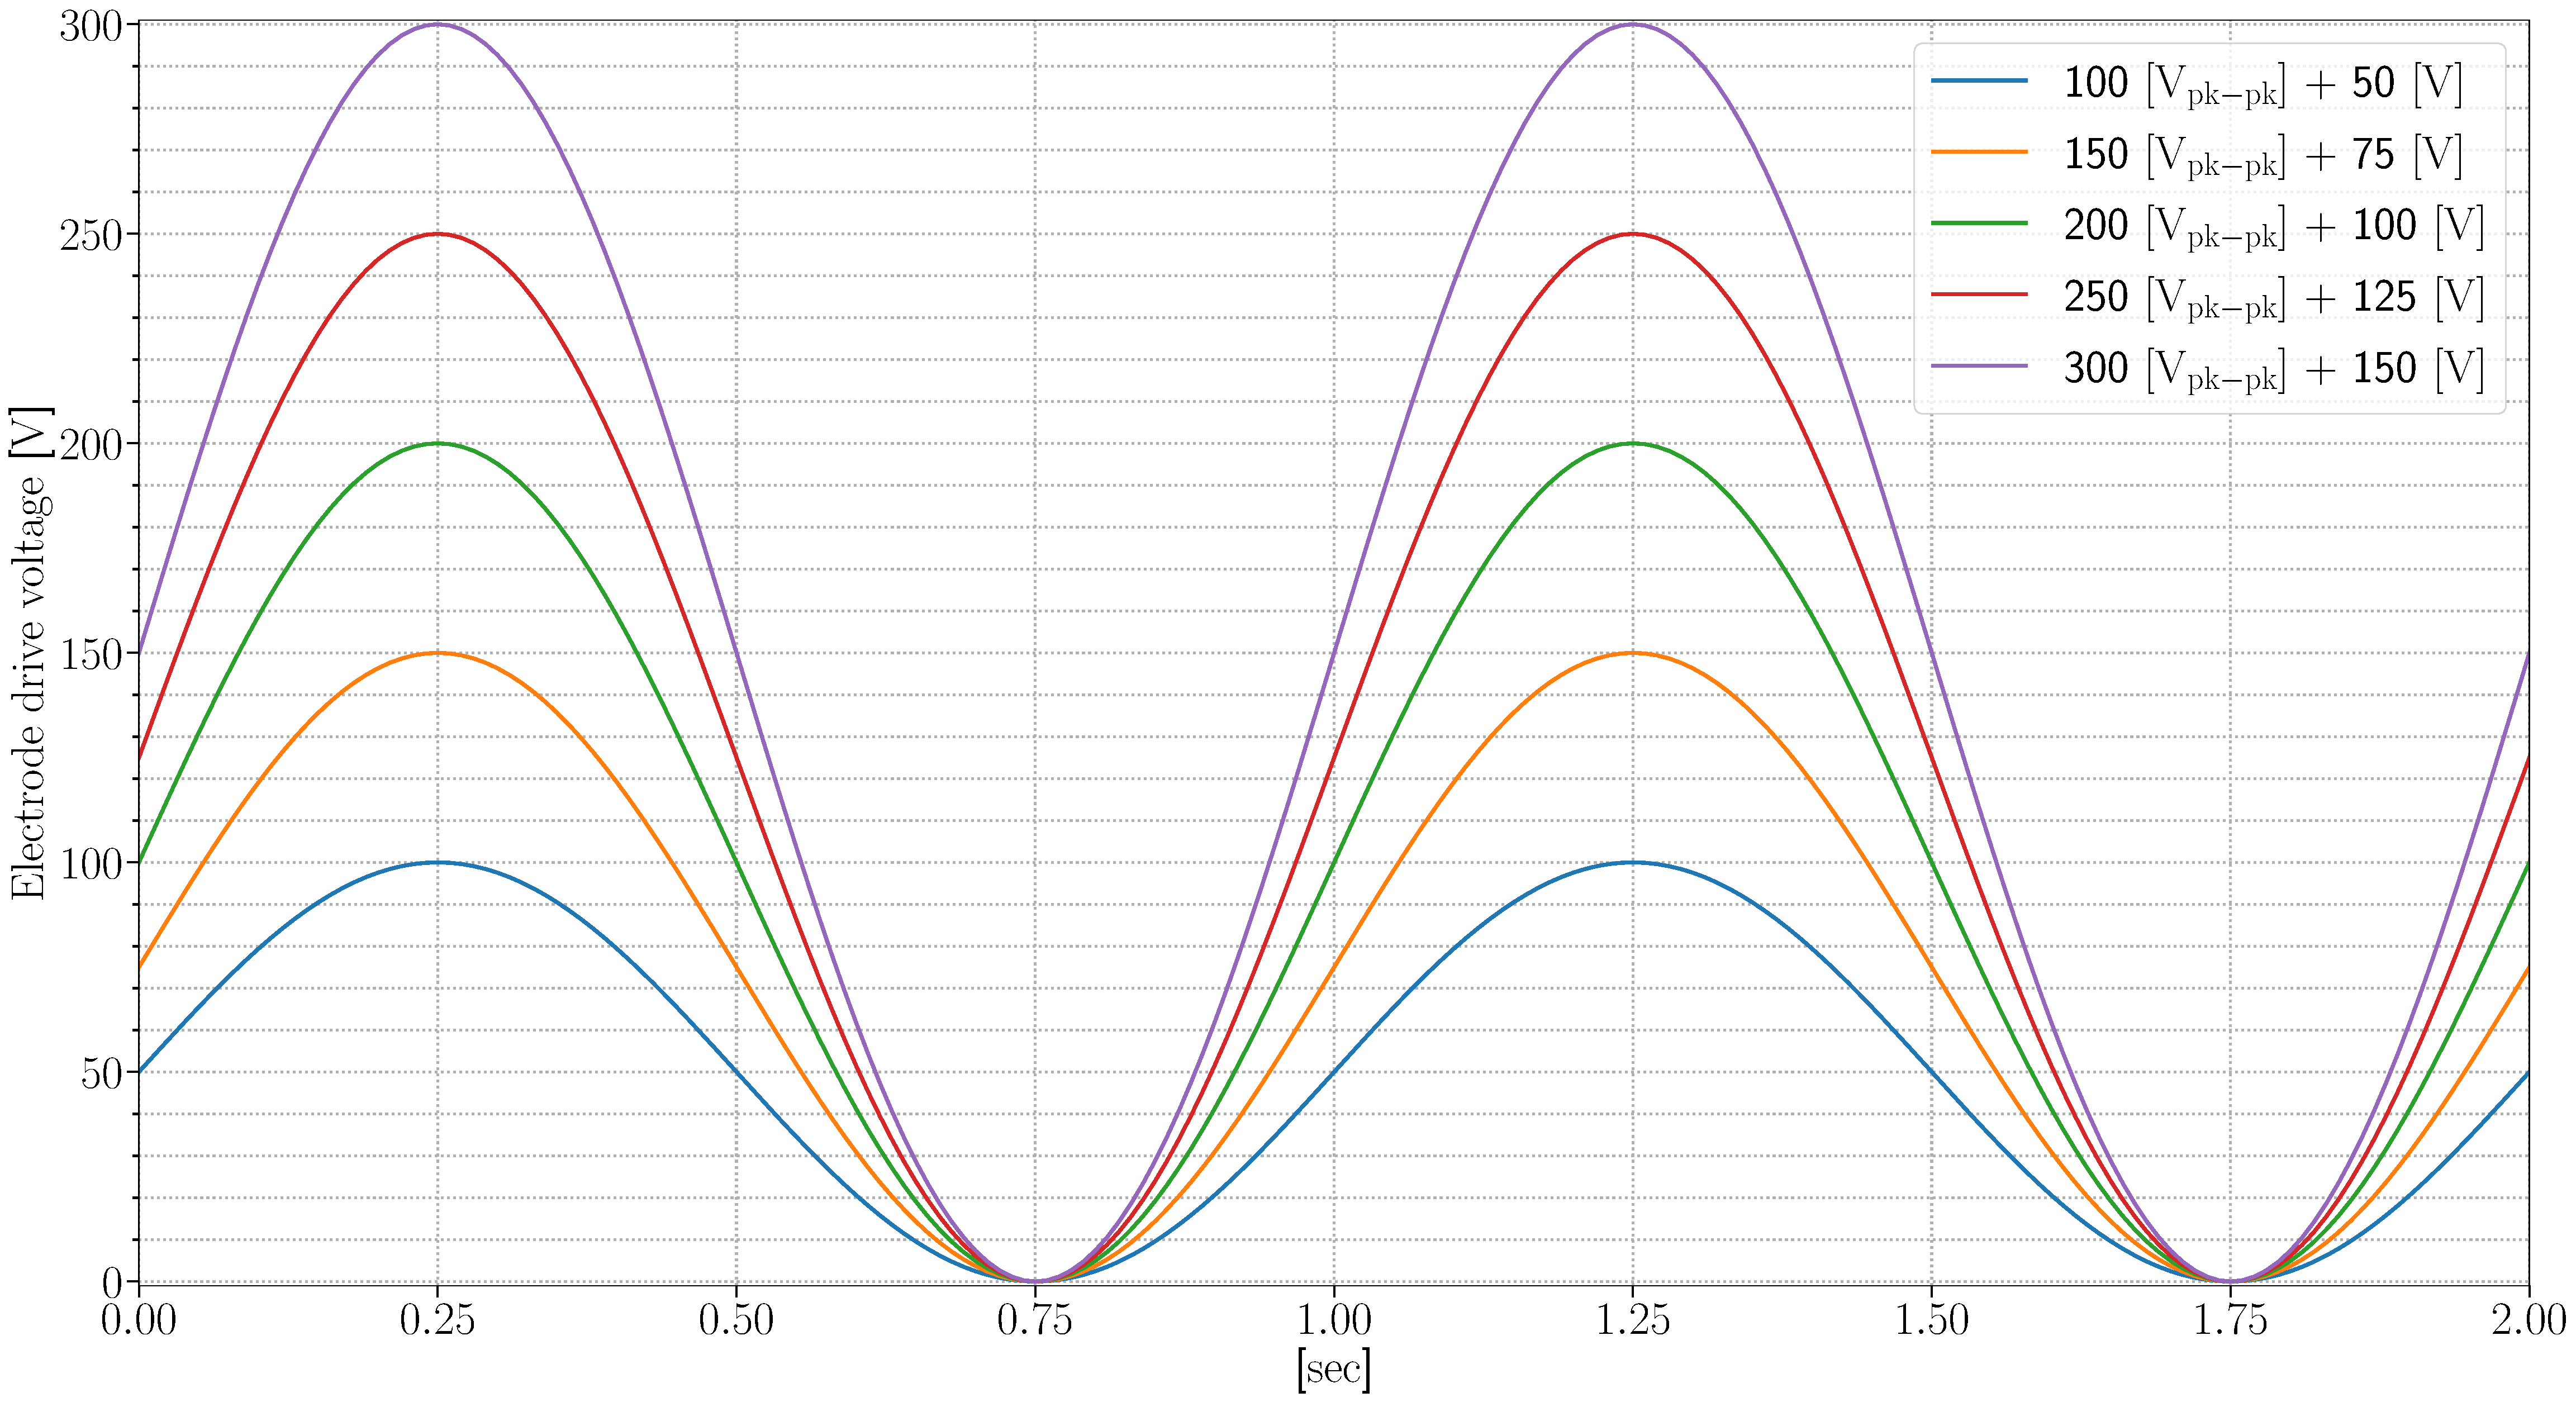
\includegraphics[width=\textwidth]{figs/ALGAAS/results_figs/assembly2/vary_daao.pdf}
    \caption{The varied drive amplitudes and offsets input into the HVA to perform the following test}
    \label{fig:vary_daao}
\end{figure}

\begin{figure}[H]
    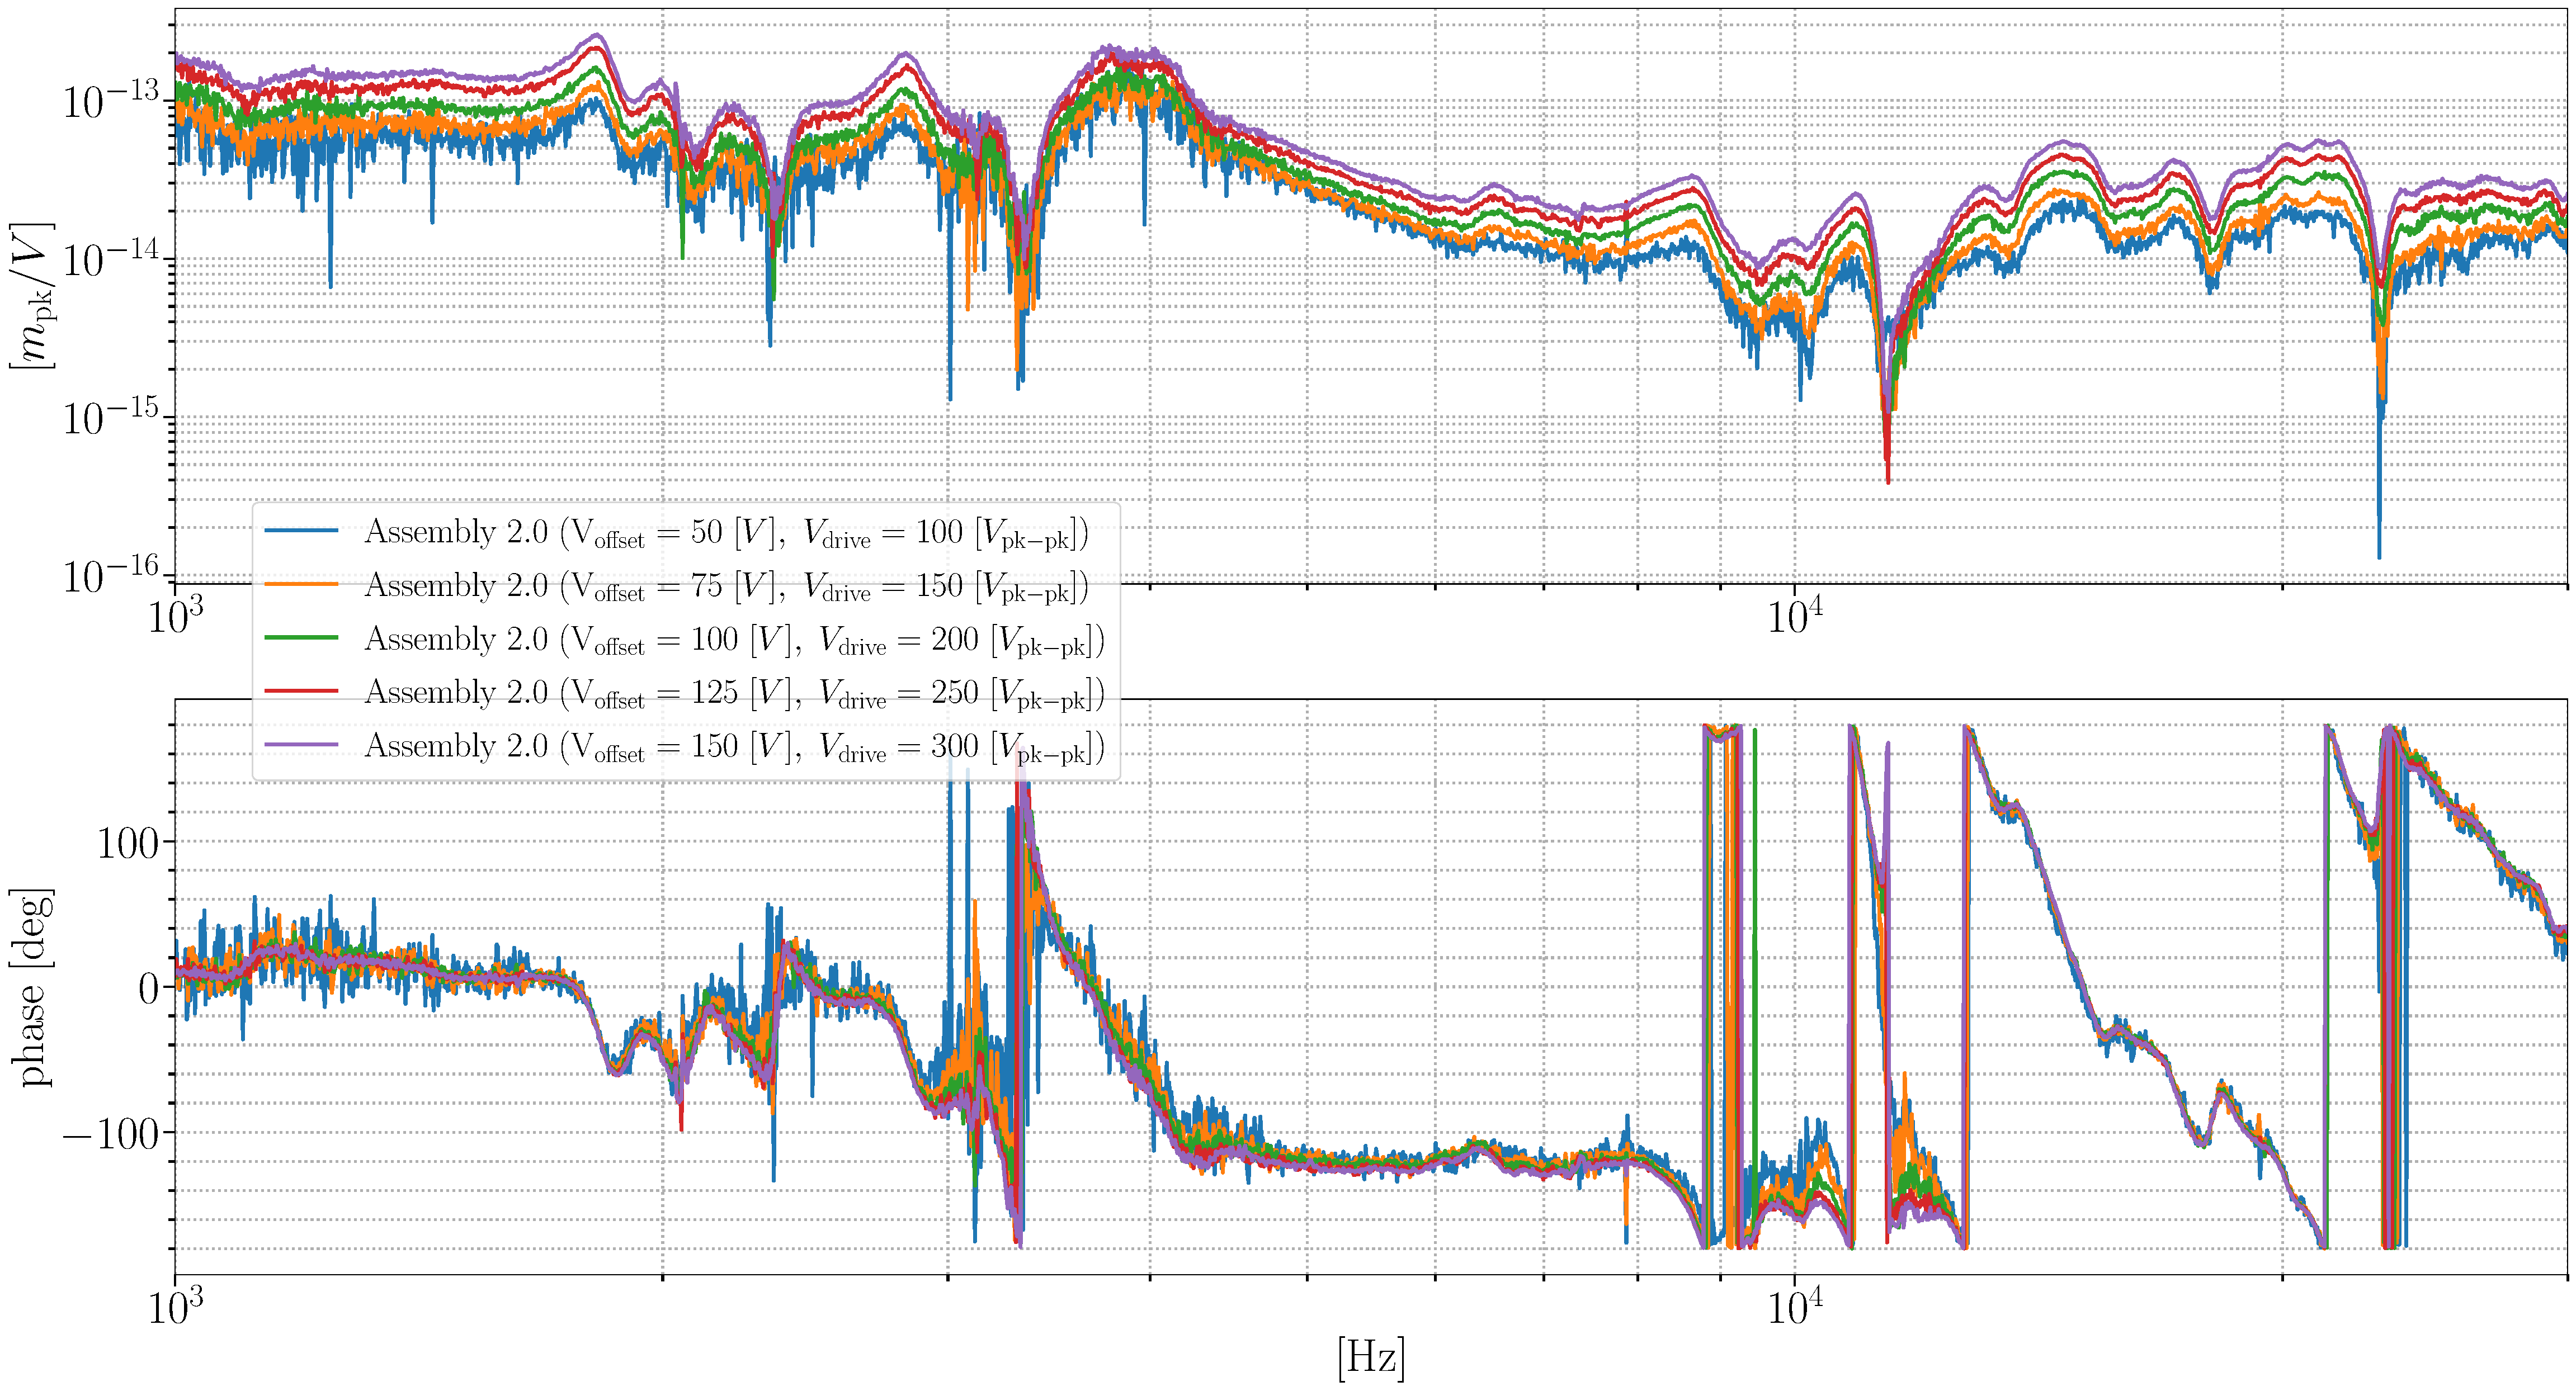
\includegraphics[width=\textwidth]{figs/ALGAAS/results_figs/assembly2/vvao517.pdf} 
    \caption{Assembly 2.0 transfer function measurements with varied drive amplitudes and offsets indicated in ~\ref{fig:vary_daao}.}
    \label{fig:vvao517}
\end{figure}

\subsubsection{Assembly 3 (MACOR mount)}
With most of the same characteristics from Assembly 3, an optical mount made of MACOR, a machinable ceramic, was constructed and installed. With the material's high Young's modulus (66.9 GPa), and a moderate Poisson ratio (.29) \cite{macor} making it by far the most durable / non-conductive mounting solution tried.

An optical mount for the sample made with MACOR, along with glass bearnings .48 $\pm$ .01 cm $\diameter$  and a McMaster-Carr 8-32, 1/2" ceramic screw were used to clamp and suspend the optical sample. A 1.24" $\diameter$ hole was bored into the MACOR with a (\textcolor{red}{depth?}) depth so that there is a .351 $\pm$ mm clearance between the front and back surface of the sample to the electrode plates.

%%FIGURE: sample in-situ
\begin{figure}[!ht]
    \begin{subcaptiongroup}
	    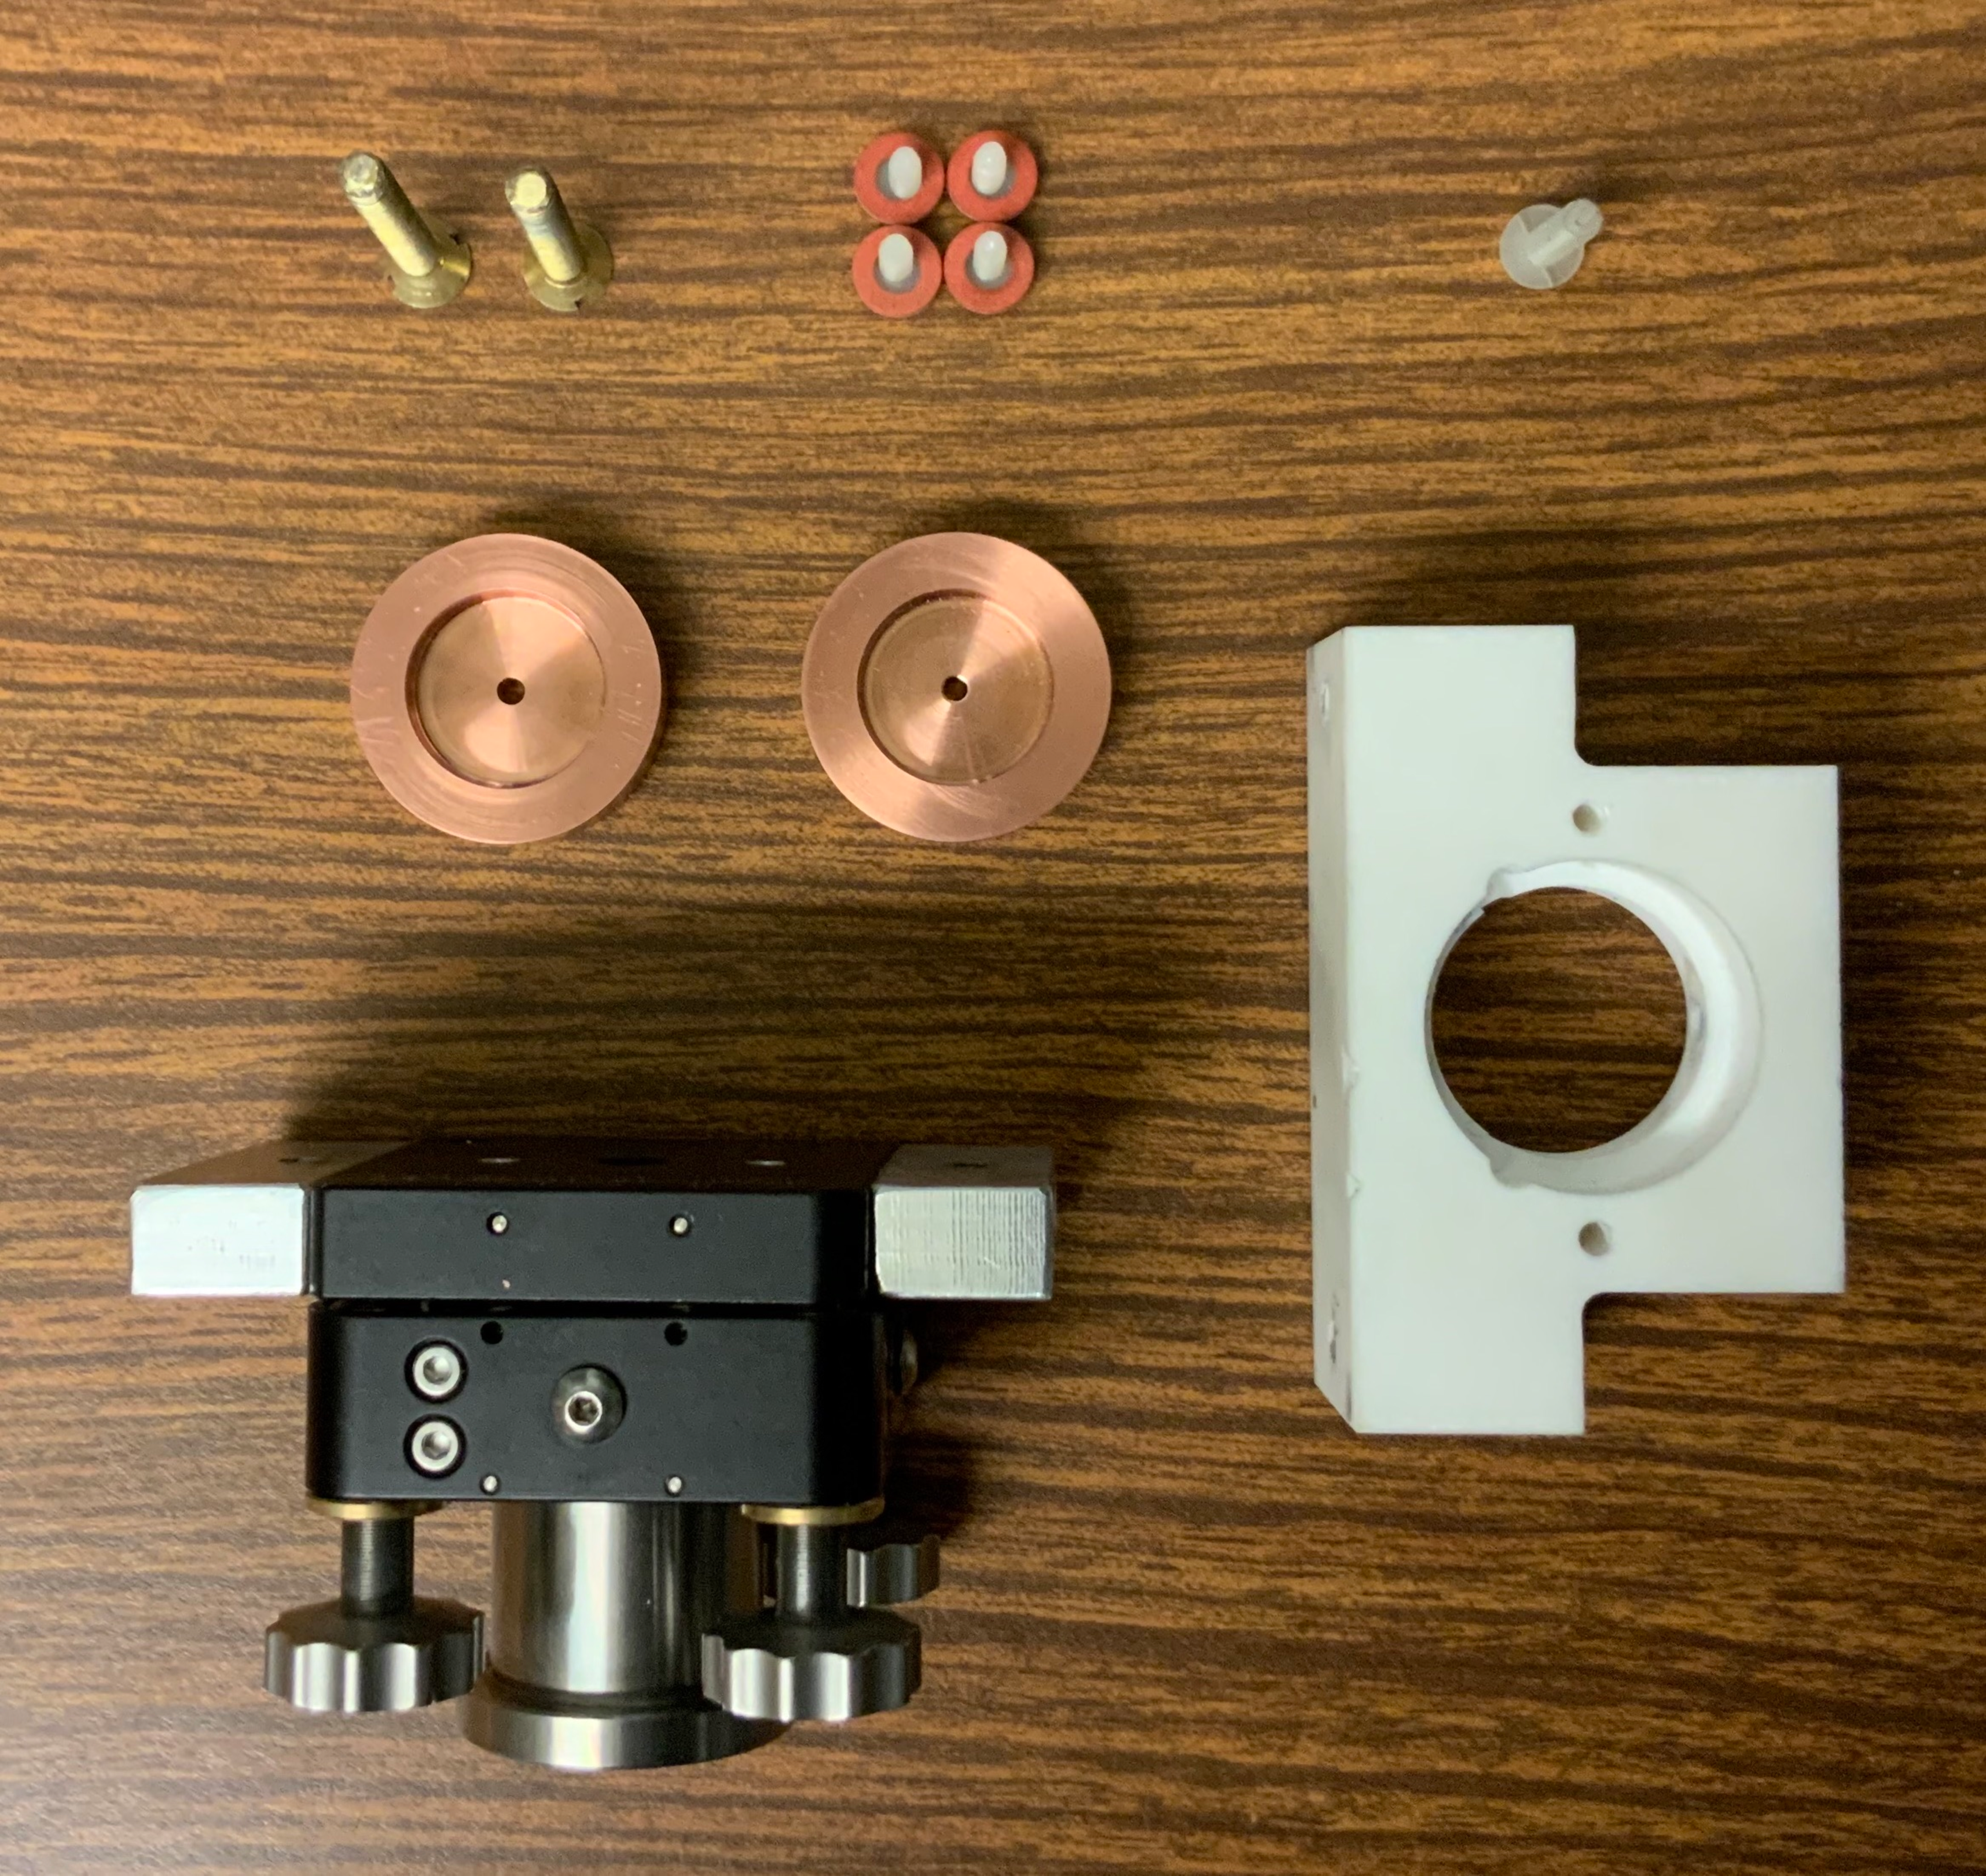
\includegraphics[width=.5\textwidth]{figs/ALGAAS/assemblies/assembly3/assembly3_disassembled.pdf}
	    \phantomcaption\label{A3_disassembled}
	    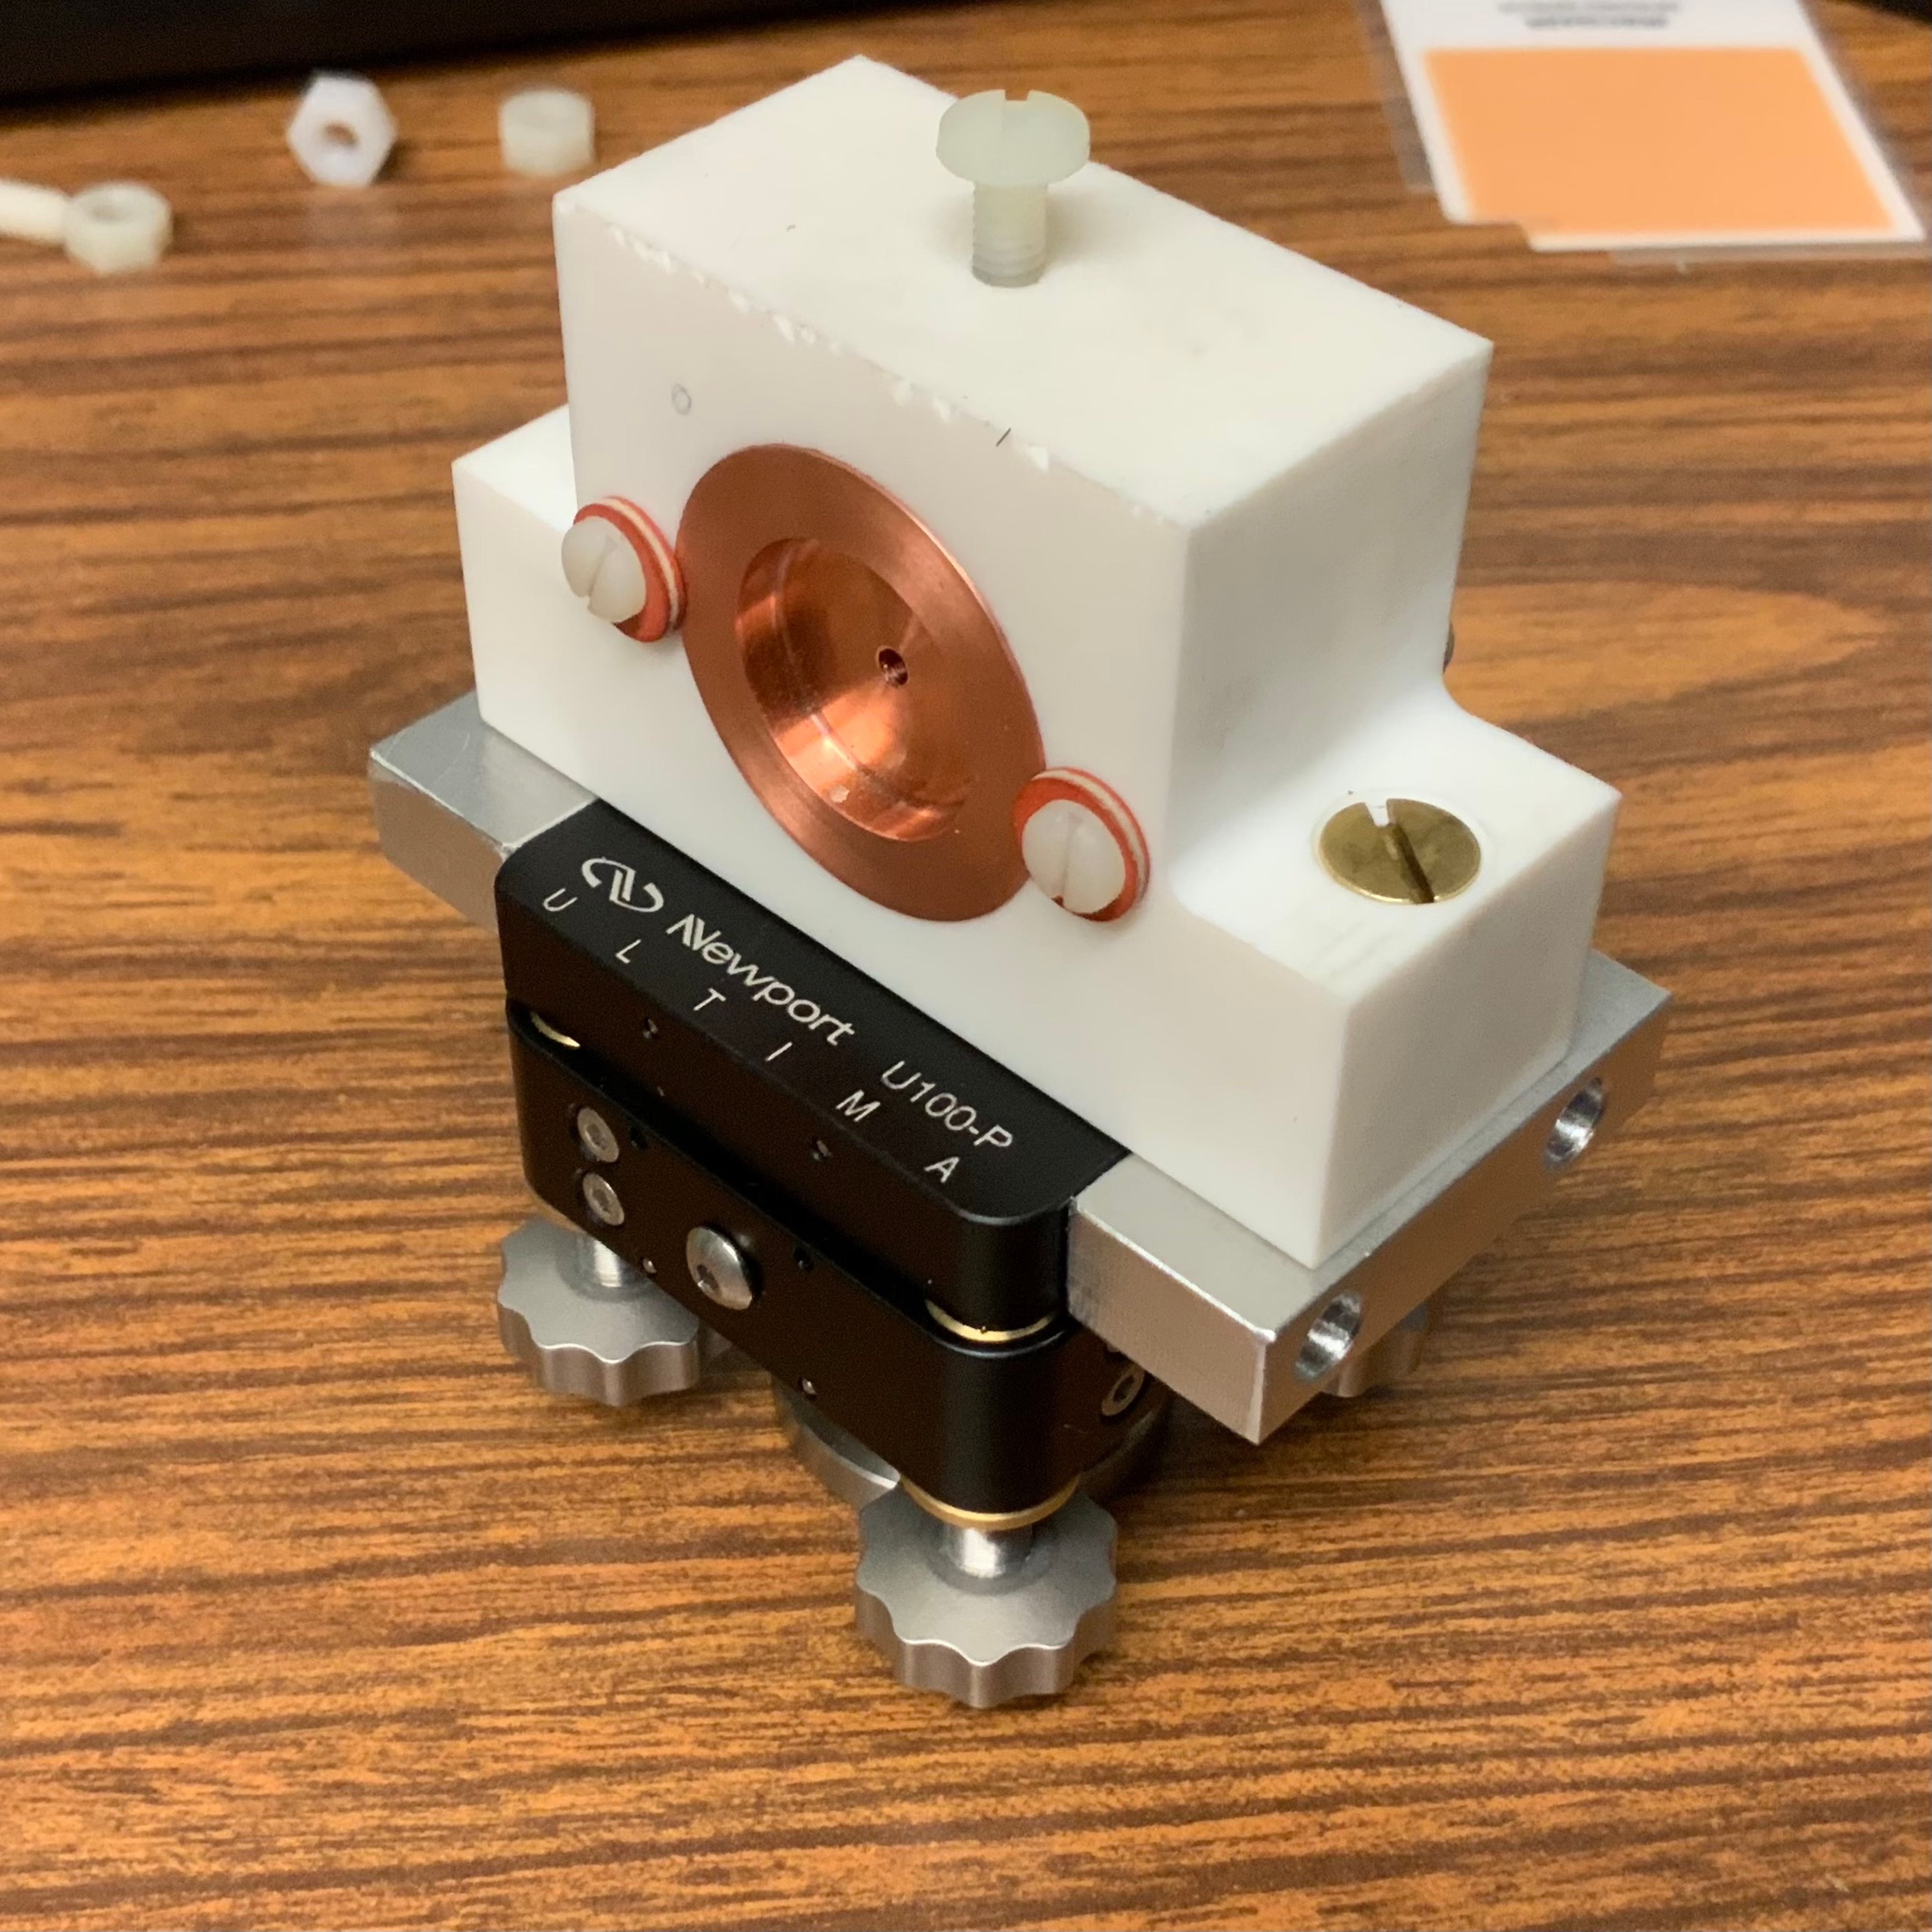
\includegraphics[width=.5\textwidth]{figs/ALGAAS/assemblies/assembly3/assembly3_isometric.pdf}
	    \phantomcaption\label{A3_isometric}
    \end{subcaptiongroup}
    \caption{Assembly 3: \subref{A3_disassembled} disassembled configuration and \subref{A3_isometric} an isometric view of the assembled configuration.}
    \label{fig:assembly3}
\end{figure}


\begin{figure}[H]
    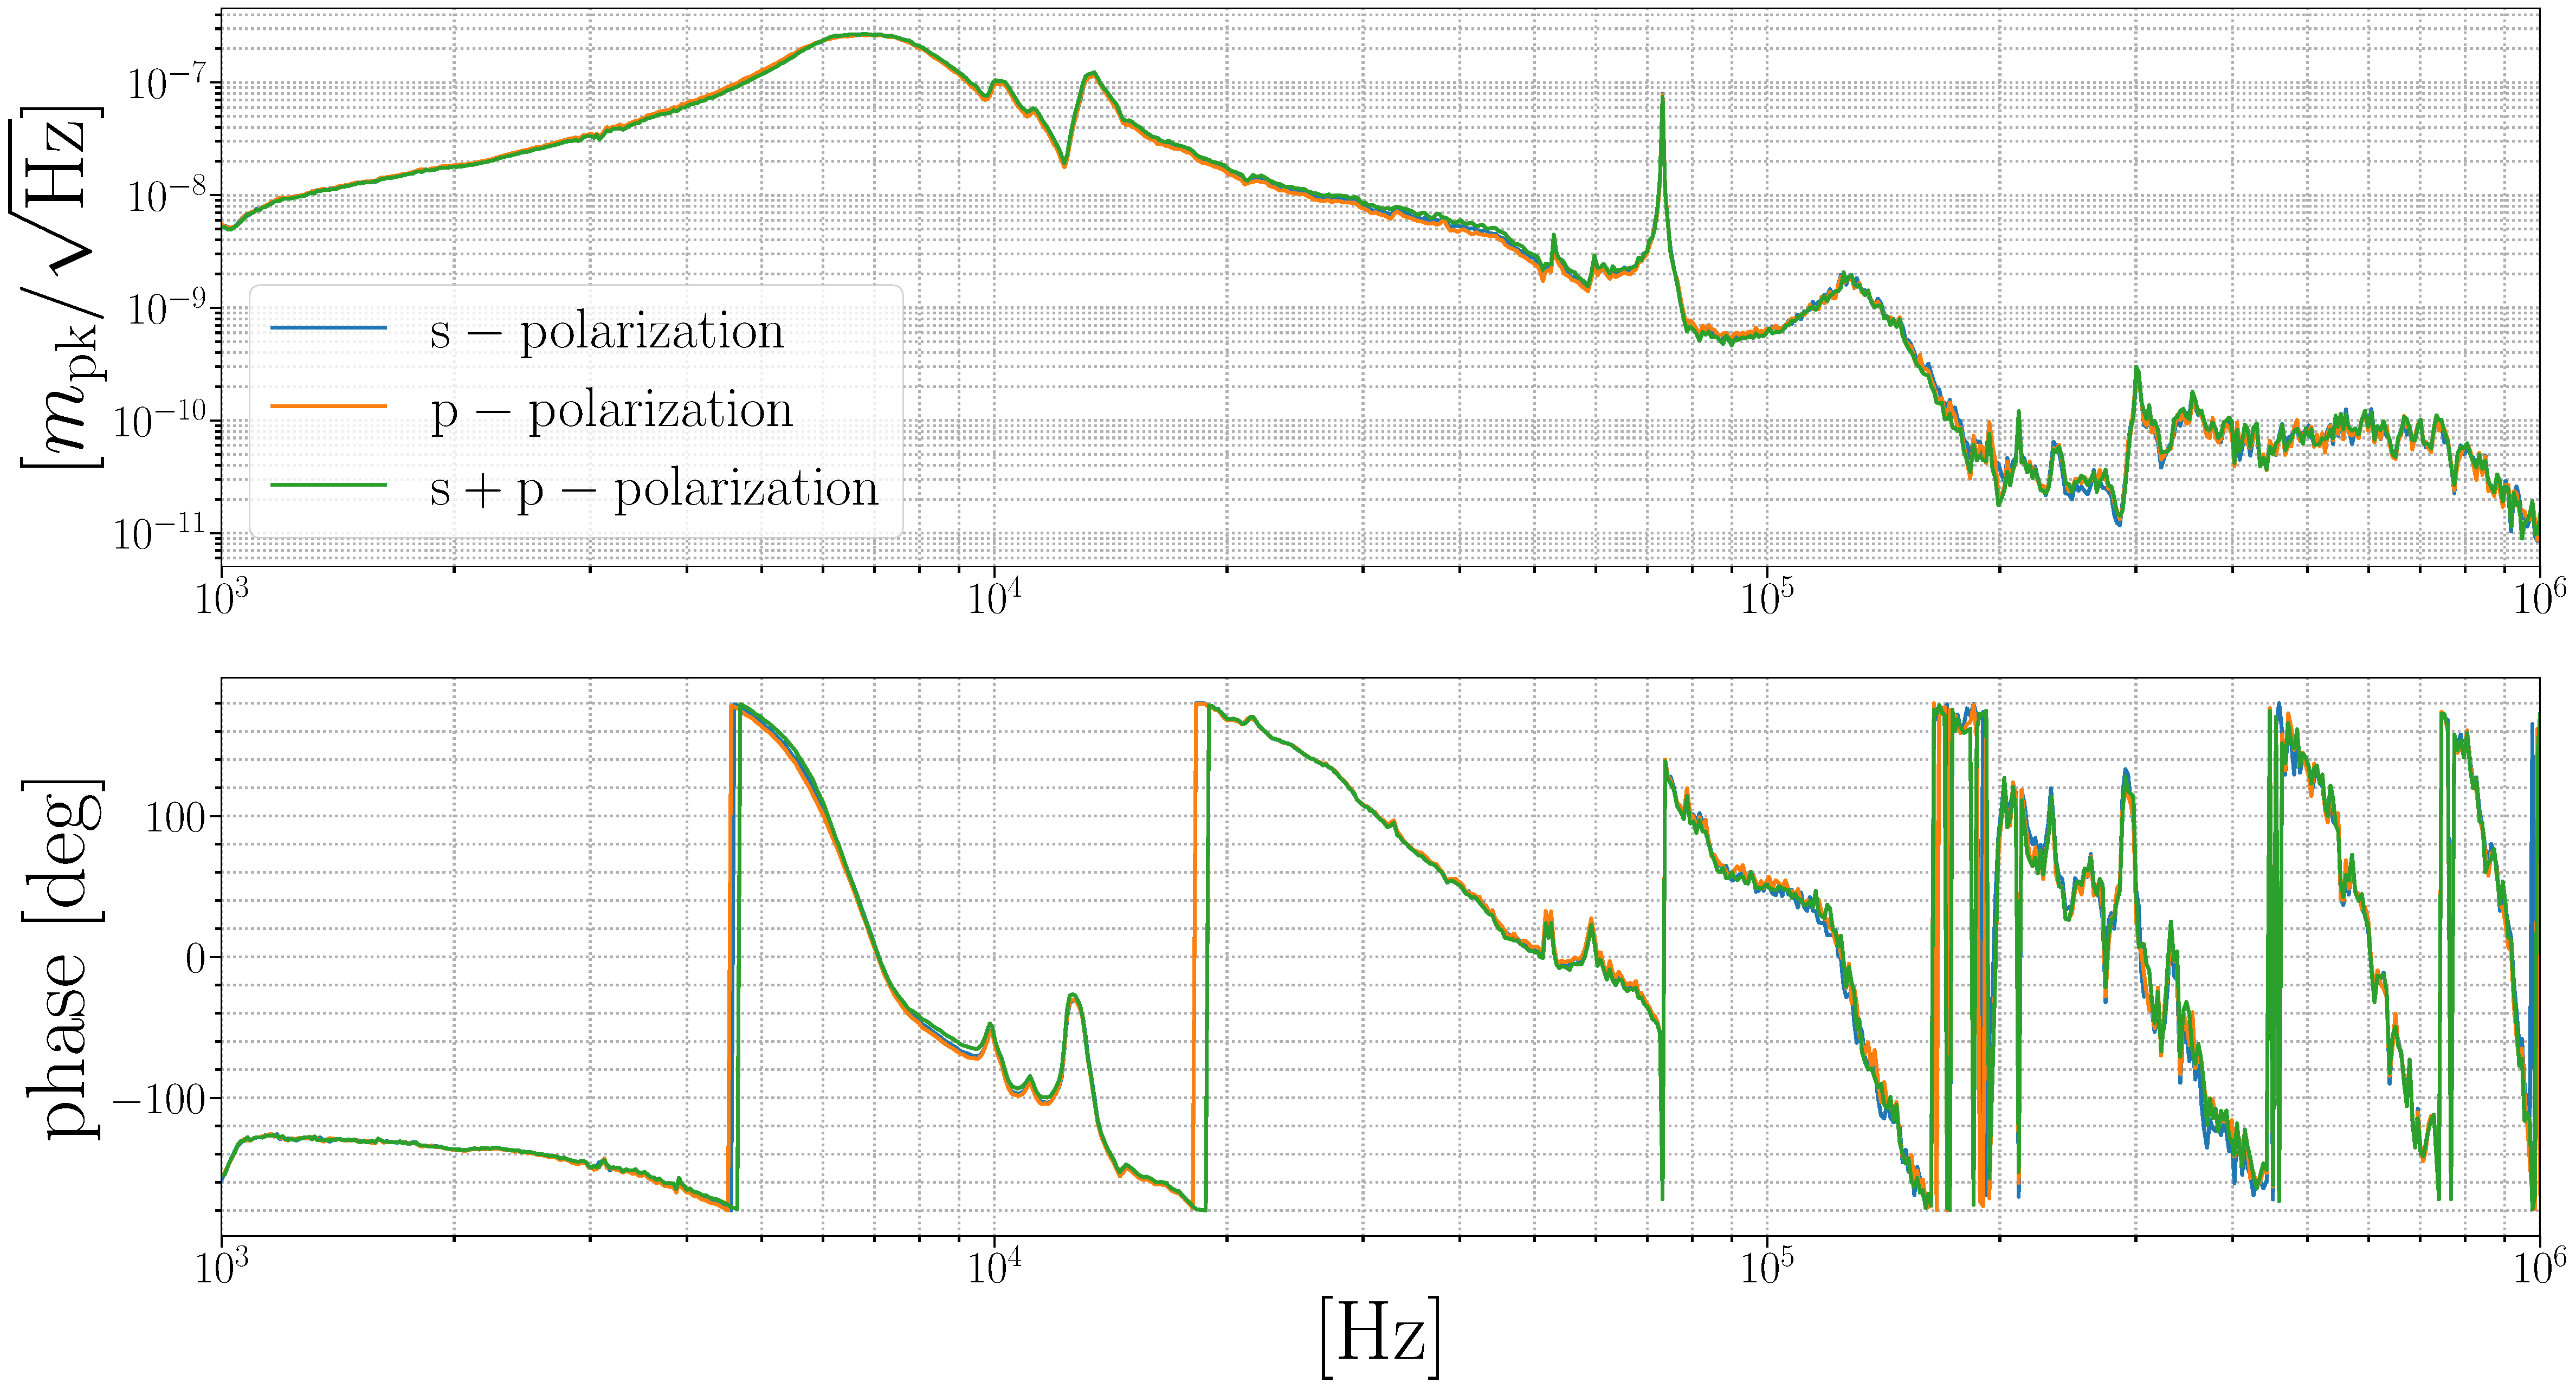
\includegraphics[width=\textwidth]{figs/ALGAAS/results_figs/assembly3/petgmsvv64.pdf}
    \caption{A polarization depdendent test using the MACOR mont}
    \label{fig:measurement_sum}
\end{figure}

\subsubsection{Opto-mechanical coupling}
During Assembly 2 tests the drive coupling seen in the transfer function measurements for all mounts tried was hypothesized to be due to mechanical action the assembly construction when driving the voltage on electrodes plates. Tracking consistent mechanical action for assemblies prior to Assembly 3 was difficult due to inconsistent mechanical settings between some measurements. More consistent measurements were realized when mechanical settings were tracked more carefully (i.e. set screw torque) and ceramic / glass materials used for suspending sample within the assembly. 
Sample and mount mechanical mode excitations. Seen with both AlGaAs and a HR coating from an AtFilm (IBS coating)
\begin{itemize}
\item \textbf{Vibration of plates (Leissa)} \cite{leissa} Computing frequencies and order of magnitude
\item \textbf{Steve's COMSOL model results}
\end{itemize}

\subsubsection{Dual-polarization locked configuration}

\subsection{Conclusion}
